\documentclass[xcolor=svgnames,9pt,english, aspectratio=169]{beamer}
%\documentclass[xcolor=svgnames,9pt,english, handout, aspectratio=169]{beamer}
\newcommand{\handout}{0}
% Shared template layer for the six decks: theme, beamer layout, and the packages
% every deck needs. Each deck inputs this near the top of its preamble, BEFORE
% ../common/theme.tex (metropolis must be selected before the palette overrides it).
%
% Notation macros and theorem environments are deliberately NOT shared. They
% conflict between the decks, and merging them would silently change symbols
% inside equations:
%   \e          decks 1-2: \bs{\epsilon}      deck 3: \boldsymbol{\eta}
%   \M          decks 1-2: \mb{M}             deck 3: \mathcal{M}
%   \blue       decks 1-2: blue               deck 3: RoyalBlue
%   \indep      different implementations
%   assumption / proposition
%               decks 1-2: own counter        deck 3: shares the theorem counter
%
% Each deck therefore keeps its own notation block. Only the look is unified.

\usetheme{metropolis}
\setbeamertemplate{navigation symbols}{}

% Deck 3's margins; decks 1 and 2 previously used 2em, which at 9pt is ~6.3mm.
\setbeamersize{text margin left=5mm, text margin right=5mm}
\setbeamertemplate{itemize/enumerate body begin}{\leftmargini=1.5em\relax}
\setbeamertemplate{itemize/enumerate subbody begin}{\leftmarginii=1.5em\relax}
\setbeamertemplate{itemize/enumerate subsubbody begin}{\leftmarginiii=1.5em\relax}

\usepackage{xcolor}
\usepackage{colortbl}
\usepackage{amsmath}
\usepackage{amsfonts}
\usepackage{amssymb}
\usepackage{graphicx}
\usepackage{multirow}
\usepackage{listings}
\usepackage{booktabs}
\usepackage{tikz}
\usetikzlibrary{arrows.meta,positioning,decorations.pathreplacing}

% Citations: one bib file at the repository root, Chicago author-date via biblatex-chicago
% (needs biber). Reference frames are generated with \printbibliography; in-text citations
% use \textcite (narrative) and \parencite (parenthetical). The CMS rule prints one to three
% names in full and four or more as "First et al."; \citeshort forces "et al.", \citeall
% prints every name (text/paren/author variants likewise). The override lasts one citation.
\usepackage{csquotes}
\usepackage[authordate,backend=biber,doi=false,url=false,isbn=false,eprint=false,
            maxbibnames=10,compresspages=true,dashed=false]{biblatex-chicago}
\addbibresource{../references.bib}
% Entry size: beamer wraps each part of a biblatex entry in its "bibliography entry author /
% title / location / note" fonts, and metropolis sets those to \normalsize, so \bibfont alone
% does not change the size. The four \setbeamerfont lines in theme.tex set the size that shows.
\renewcommand*{\bibfont}{\scriptsize}
\setlength{\bibitemsep}{0.7em}   % visible air between entries
\setlength{\bibhang}{0.5em}
% The References frame of every deck: \begin{frame}[t,allowframebreaks=1.0] ... \referencelist.
% Beamer's automatic break for this list fires at about two thirds of the frame; the factor
% 1.1 lets it fill the frame. The small negative skip closes the list's top gap.
\newcommand{\referencelist}{\vspace*{-0.6em}\printbibliography[heading=none]}
\newcommand{\citeshort}[1]{\AtNextCitekey{\defcounter{maxnames}{1}}\cite{#1}}
\newcommand{\textciteshort}[1]{\AtNextCitekey{\defcounter{maxnames}{1}}\textcite{#1}}
\newcommand{\parenciteshort}[1]{\AtNextCitekey{\defcounter{maxnames}{1}}\parencite{#1}}
\newcommand{\citeauthorshort}[1]{\AtNextCitekey{\defcounter{maxnames}{1}}\citeauthor{#1}}
\newcommand{\citeall}[1]{\AtNextCitekey{\defcounter{maxnames}{9}}\cite{#1}}
\newcommand{\textciteall}[1]{\AtNextCitekey{\defcounter{maxnames}{9}}\textcite{#1}}
\newcommand{\parenciteall}[1]{\AtNextCitekey{\defcounter{maxnames}{9}}\parencite{#1}}
% PDF metadata: beamer copies the whole \author box into the author field; set it plainly
% once every deck-level \author has run (etoolbox's end-of-preamble hook).
\AtEndPreamble{\hypersetup{pdfauthor={Yiqing Xu}}}
   % theme, layout, packages

\setbeamertemplate{footline}[frame number]{}

\graphicspath{{./figs/}}%

\usepackage{makecell}
% Shared visual system for the six decks: palette, fonts, footline.
% Swap the four colors below to rebrand every deck at once.
\definecolor{SlideRed}{HTML}{9E1B32}
\definecolor{SlideInk}{HTML}{252A34}
\definecolor{SlideBlue}{HTML}{2F6B9A}
\definecolor{SlideMist}{HTML}{F8F3F3}


\setbeamercolor{normal text}{fg=SlideInk,bg=white}
\setbeamercolor{structure}{fg=SlideRed}
\setbeamercolor{alerted text}{fg=SlideRed}
\setbeamercolor{frametitle}{fg=white,bg=SlideRed}
\setbeamercolor{title}{fg=SlideRed}
\setbeamercolor{subtitle}{fg=SlideInk}
\setbeamercolor{block title}{fg=white,bg=SlideRed}
\setbeamercolor{block body}{fg=SlideInk,bg=SlideMist}
\setbeamercolor{section in toc}{fg=SlideRed}

\setbeamerfont{title}{series=\bfseries,size=\Large}
\setbeamerfont{frametitle}{series=\bfseries,size=\large}
\setbeamerfont{block title}{series=\bfseries}
\setbeamertemplate{navigation symbols}{}
\setbeamertemplate{items}[circle]
\setbeamertemplate{blocks}[rounded][shadow=false]
\setbeamertemplate{bibliography item}{}   % no document icons on the References frames
\setbeamertemplate{frametitle continuation}{}
\setbeamertemplate{footline}{%
  \leavevmode\hbox{%
  \begin{beamercolorbox}[wd=.88\paperwidth,ht=2.6ex,dp=1.2ex,leftskip=1.2em]{author in head/foot}%
  \usebeamerfont{author in head/foot}\insertshorttitle
  \end{beamercolorbox}%
  \begin{beamercolorbox}[wd=.12\paperwidth,ht=2.6ex,dp=1.2ex,center]{date in head/foot}%
  \insertframenumber
  \end{beamercolorbox}}}

\newcommand{\slidesource}[1]{\vfill{\scriptsize\color{gray}Source: #1}}
\newcommand{\keyquestion}[1]{\begin{block}{Question}#1\end{block}}


\title{Panel Methods (5): Modern DID}
\subtitle{Lectures on Causal Panel Analysis}
\author{Yiqing Xu\\\smallskip Stanford University}
\date{September 2026}

% ---------- notation (deck-local; do not merge across decks) ----------
\newcommand{\E}{\ensuremath{\mathbb{E}}}

% ---------- treatment-grid colors ----------
\definecolor{cellC}{HTML}{8FD8F8}   % under control
\definecolor{cellT}{HTML}{0F4C81}   % under treatment
\definecolor{cellP}{HTML}{FBDCEE}   % comparison cells in use
\definecolor{cellG}{HTML}{A2426F}   % target cells being estimated

% one cell: \gcell{col}{row}{color}, col 1-6 left-right, row 1-5 top-bottom (A-E)
\newcommand{\gcell}[3]{\fill[#3] ({#1-1},{5-#2}) rectangle ({#1},{6-#2});}
% base staggered pattern: A,B treated from 3; C from 5; D from 6; E never
\newcommand{\basegrid}{%
  \fill[cellC] (0,0) rectangle (6,5);
  \foreach \c in {3,...,6} {\gcell{\c}{1}{cellT}\gcell{\c}{2}{cellT}}
  \foreach \c in {5,6} {\gcell{\c}{3}{cellT}}
  \gcell{6}{4}{cellT}}
% grid frame + labels (draw last so lines sit on top of fills)
\newcommand{\gridframe}{%
  \draw[white, very thin] (0,0) grid (6,5);
  \draw[gray!60, thin] (0,0) rectangle (6,5);
  \foreach \r/\l in {1/A,2/B,3/C,4/D,5/E} {\node[left=2pt] at (0,{5.5-\r}) {\small \l};}
  \foreach \c in {1,...,6} {\node[below=2pt] at ({\c-0.5},0) {\small \c};}}
% general pattern with treatment reversal (PanelMatch / imputation demos, from the Chicago
% deck): A on 4-5; B on 3-4; C on 5-6; D on 1 and 3; E never
\newcommand{\generalgrid}{%
  \fill[cellC] (0,0) rectangle (6,5);
  \gcell{4}{1}{cellT}\gcell{5}{1}{cellT}
  \gcell{3}{2}{cellT}\gcell{4}{2}{cellT}
  \gcell{5}{3}{cellT}\gcell{6}{3}{cellT}
  \gcell{1}{4}{cellT}\gcell{3}{4}{cellT}}
% grid frame with row labels only (column labels are placed per frame)
\newcommand{\gridframerows}{%
  \draw[white, very thin] (0,0) grid (6,5);
  \draw[gray!60, thin] (0,0) rectangle (6,5);
  \foreach \r/\l in {1/A,2/B,3/C,4/D,5/E} {\node[left=2pt] at (0,{5.5-\r}) {\small \l};}}
% stacked-DID cohort block with bottom-left corner (#1,#2): #3 cohort rows treated from
% column #4 (1-6), plus one never-treated row at the bottom (the copy of E)
\newcommand{\cblock}[4]{%
  \fill[cellC] (#1,#2) rectangle ({#1+6},{#2+#3+1});
  \fill[cellT] ({#1+#4-1},{#2+1}) rectangle ({#1+6},{#2+#3+1});
  \draw[white, very thin] (#1,#2) grid ({#1+6},{#2+#3+1});
  \draw[gray!60, thin] (#1,#2) rectangle ({#1+6},{#2+#3+1});}

\begin{document}

\AtBeginSection[]
{
  \begin{frame}<beamer>
    \frametitle{Outline}
    \tableofcontents[currentsection]
  \end{frame}
}

\begin{frame}
  \titlepage
  \thispagestyle{empty}
  \addtocounter{framenumber}{-1}
\end{frame}

\begin{frame}
  \frametitle{The Six Lectures}
\begin{center}
\begin{tikzpicture}[
  lecture/.style={rounded corners=3pt, draw=SlideRed, thick,
                  minimum height=1.6cm, text width=2.6cm,
                  align=center, inner sep=5pt},
  link/.style={-{Latex[length=2.2mm]}, thick, draw=SlideInk}
]
\node[lecture, fill=SlideMist] (l1) at (0,0)
  {\textbf{1. Parametric panel models}\\[0.25em]
   \footnotesize FE regressions and their assumptions};
\node[lecture, fill=SlideMist] (l2) at (0,-2.9)
  {\textbf{2. Difference-in-differences}\\[0.25em]
   \footnotesize The canonical design and identification};
\node[lecture, fill=SlideMist] (l3) at (3.9,0)
  {\textbf{3. Factorial DID}\\[0.25em]
   \footnotesize When the event affects everyone};
\node[lecture, fill=SlideMist] (l4) at (3.9,-2.9)
  {\textbf{4. TWFE revisited}\\[0.25em]
   \footnotesize What breaks under staggered timing};
\node[lecture, fill=SlideRed!25, very thick] (l5) at (7.8,0)
  {\textbf{5. Modern DID}\\[0.25em]
   \footnotesize Heterogeneity-robust estimators};
\node[lecture, fill=SlideMist] (l6) at (7.8,-2.9)
  {\textbf{6. Synthetic control \& factor models}\\[0.25em]
   \footnotesize Imputing treated counterfactuals};
\draw[link] (l1) -- (l2);
\draw[link] (l2.east) -- ++(0.5,0) |- (l3.west);
\draw[link] (l3) -- (l4);
\draw[link] (l4.east) -- ++(0.5,0) |- (l5.west);
\draw[link] (l5) -- (l6);
\end{tikzpicture}
\end{center}
\end{frame}

\begin{frame}
  \frametitle{Where We Are}
\begin{itemize}[<+->]\itemsep1em
\item Lecture 4 diagnosed the problem: TWFE on staggered panels mixes clean and contaminated comparisons, and parallel trends failures are common
\item This lecture is about the remedies:
\begin{itemize}\itemsep0.5em
  \item A tour of the \alert{HTE-robust estimators}: what each one compares, and when each applies
  \item The \alert{diagnostics} that come with the imputation approach
  \item Three worked examples, and what we learned from \alert{reanalyzing 49 published studies} with these tools
\end{itemize}
\item Lecture 6 introduces low-rank methods, synthetic control and factor models, that can address some parallel trends violations
\end{itemize}
\end{frame}

\begin{frame}[t]
  \frametitle{Review: What Goes Wrong under Heterogeneous Effects}
\begin{itemize}\itemsep0.3em
\item<1-> Three units: $A$ never treated, $B$ treated from period 7, $C$ from period 11; solid $=$ observed, dashed $=$ the untreated trajectory $Y(0)$
\item<2-> \alert{Result} (\cite{goodman2021difference} and others): with heterogeneous effects, TWFE need not recover any convex combination of the individual effects, even when parallel trends holds
\item<3-> \alert{Intuition}: in the boxed periods, $B$'s treated observations serve as the comparison for $C$, the ``forbidden comparison''; harmless while $B$'s effect is constant, biased once it keeps growing
\item<3-> The estimators in this lecture avoid such comparisons by construction
\end{itemize}
\vspace{-0.5em}
\begin{columns}[T,onlytextwidth]
\begin{column}{0.49\textwidth}\centering
{\footnotesize constant effects}\par
\only<1-2| handout:0>{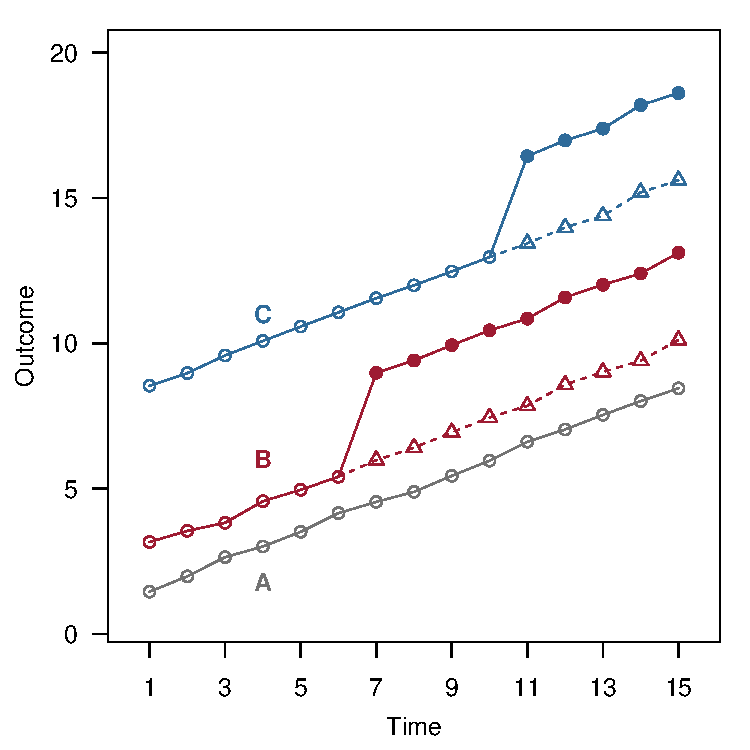
\includegraphics[height=0.4\textheight]{toy_hte_const.pdf}}%
\only<3-| handout:1>{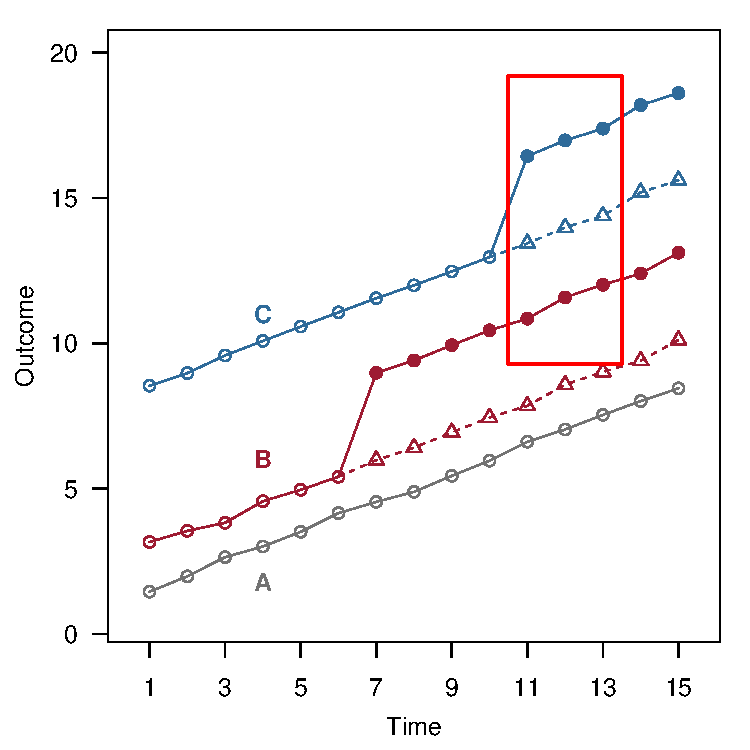
\includegraphics[height=0.4\textheight]{toy_hte_const_box.pdf}}
\end{column}
\begin{column}{0.49\textwidth}\centering
\onslide<2->{{\footnotesize effects that grow ($B$) or fade ($C$)}\par
\only<2| handout:0>{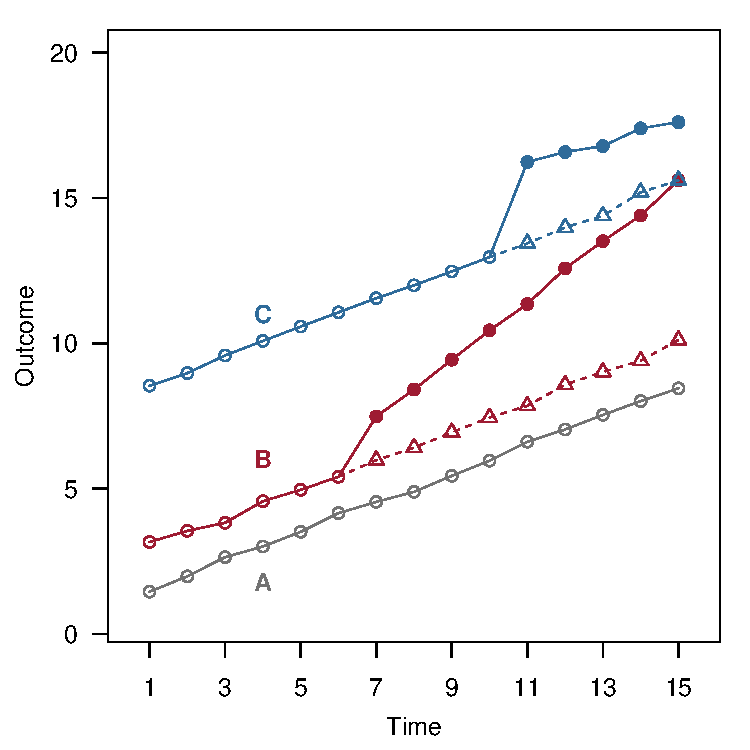
\includegraphics[height=0.4\textheight]{toy_hte_dynamic.pdf}}%
\only<3-| handout:1>{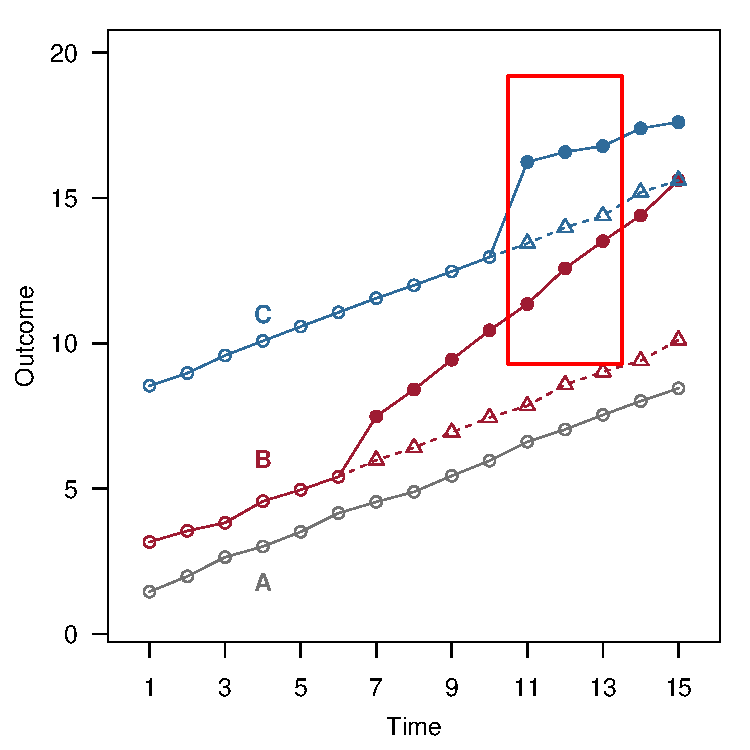
\includegraphics[height=0.4\textheight]{toy_hte_dynamic_box.pdf}}}
\end{column}
\end{columns}
\end{frame}

\begin{frame}[t]
  \frametitle{\ldots and It Compounds with Reversal and Carryover}
\begin{itemize}\itemsep0.3em
\item<1-> Most political science panels have \alert{treatment reversal}: here $B$ is treated in periods 7--11 and then exits, and $C$ switches on twice
\item<1-> In the boxed window, $B$ and $C$ serve as comparisons for each other while both are treated
\item<2-> Effects that build up and \alert{linger after exit} (carryover) make it worse: the post-exit periods are no longer clean comparisons either
\item<3-> Add parallel trends violations and anticipation, and the single-coefficient TWFE regression stands little chance; we need estimators that say \alert{which cells compare with which}
\end{itemize}
\vspace{-0.5em}
\begin{columns}[T,onlytextwidth]
\begin{column}{0.49\textwidth}\centering
{\footnotesize effects switch off with the treatment}\par
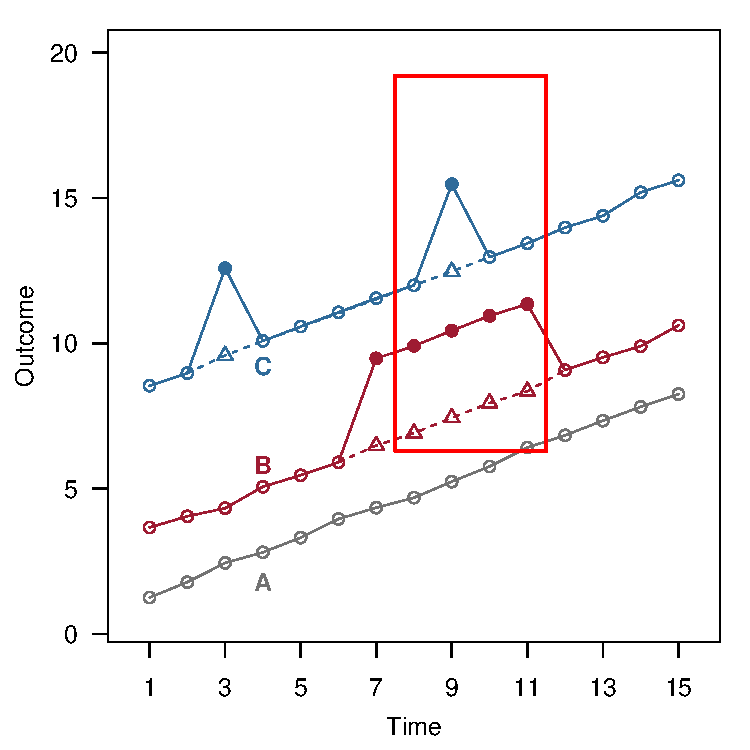
\includegraphics[height=0.4\textheight]{toy_general_ideal.pdf}
\end{column}
\begin{column}{0.49\textwidth}\centering
\onslide<2->{{\footnotesize effects build up and linger after exit}\par
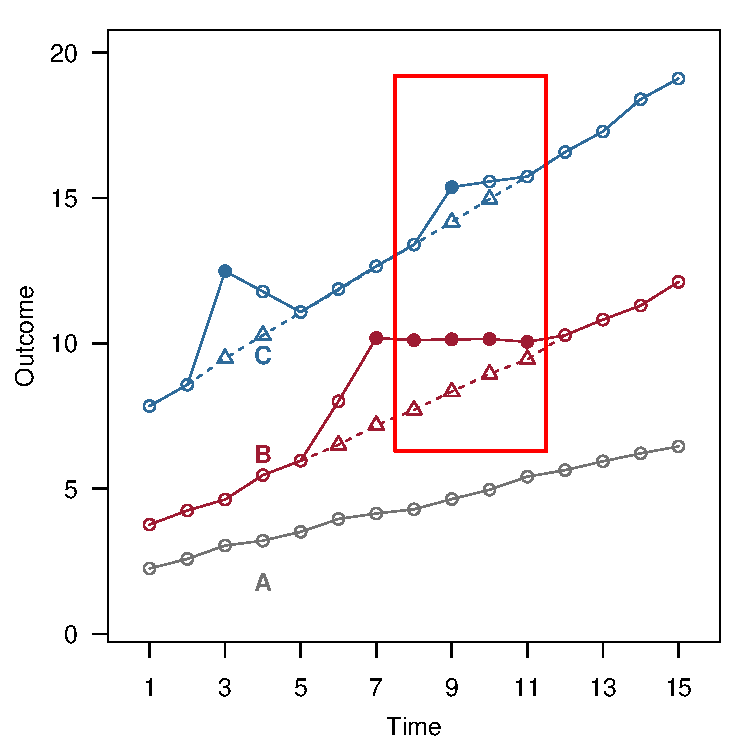
\includegraphics[height=0.4\textheight]{toy_general_carryover.pdf}}
\end{column}
\end{columns}
\end{frame}

\begin{frame}
  \frametitle{The Menu Has Grown}
\begin{columns}[c]
\begin{column}{0.5\textwidth}
\begin{center}
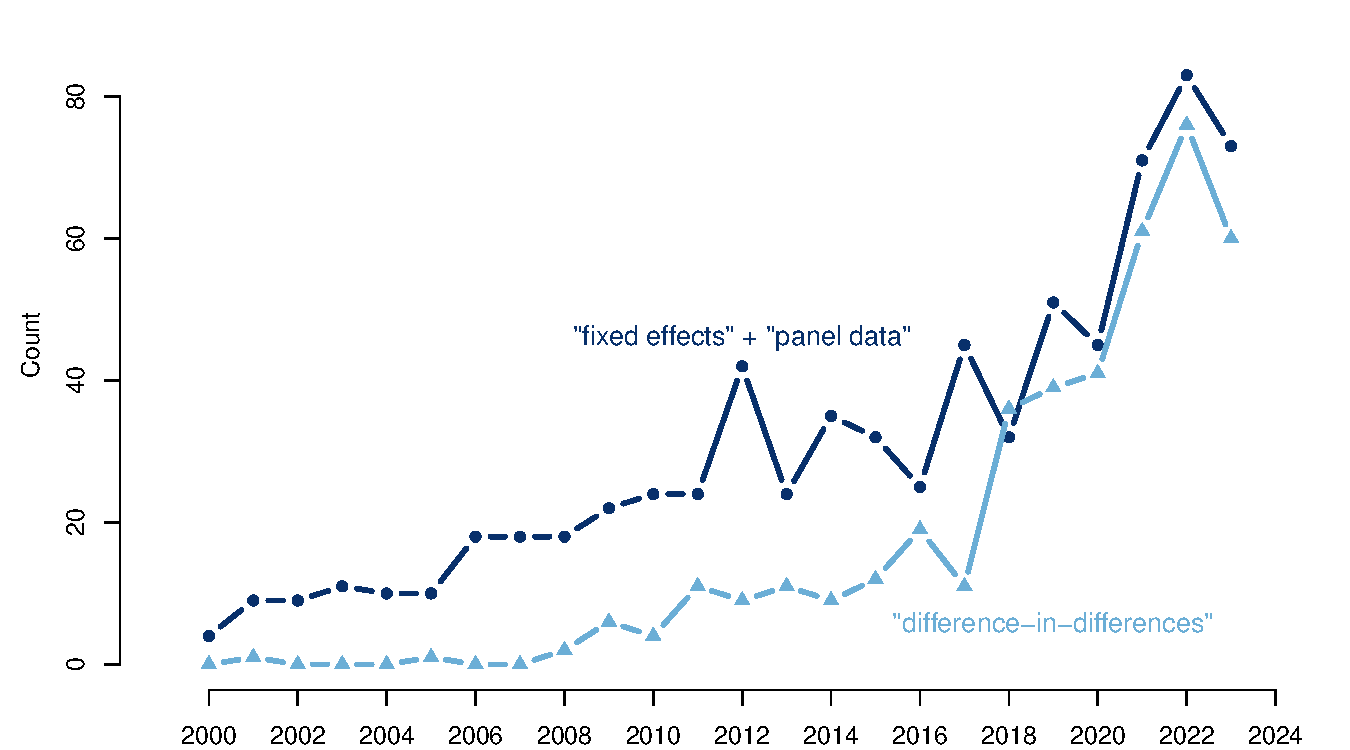
\includegraphics[width=\linewidth]{journal2.pdf}
\end{center}
\end{column}
\begin{column}{0.47\textwidth}
\begin{itemize}[<+->]\itemsep1em
\item In our review of top political science journals, 77\% of panel papers use FE models, mostly TWFE
\item The econometric critiques produced many new estimators in a short span
\item This lecture: a map of that menu, organized by \alert{which cells each estimator compares}
\end{itemize}
\end{column}
\end{columns}
\end{frame}

\begin{frame}
  \frametitle{Preview: What the Reanalyses Will Show}
\begin{center}
\begin{tikzpicture}[
  pbox/.style={draw=SlideRed, thick, fill=SlideMist, rounded corners=3pt, inner sep=7pt,
               text width=6.3cm, align=left, font=\footnotesize},
  parrow/.style={-{Latex[length=2.5mm]}, line width=1.4pt, SlideRed}]
\useasboundingbox (-0.1,-6.6) rectangle (14.7,0.1);
\node[pbox, anchor=north west] (b1) at (0,0) {%
  {\color{SlideRed}\bfseries Common practice}\\[2pt]
  $\bullet$ Fixed effects models in 77\% of panel papers, TWFE in 58\%\\
  $\bullet$ Cluster-robust SEs in 98\% of the reanalyzed studies; a cluster bootstrap in 16\%\\
  $\bullet$ Some plot of the raw data in 65\%};
\only<2->{\node[pbox, anchor=north west] (b2) at (0,-2.9) {%
  {\color{SlideRed}\bfseries Do the results hold up? Yes and no}\\[2pt]
  $\bullet$ Yes: HTE-robust estimators \alert{rarely} flip signs\\
  $\bullet$ No: parallel trends violations are still common\\
  $\bullet$ No: power runs out once the estimator is HTE-robust\\
  $\bullet$ No: few findings survive a \alert{mild} sensitivity analysis\\[2pt]
  Strong empirical support for fewer than a third of the findings};
\draw[parrow] (b1.south) -- (b2.north);}
\only<3->{\node[pbox, anchor=west] (b3) at (8.0,-3.0) {%
  {\color{SlideRed}\bfseries Takeaways}\\[2pt]
  $\bullet$ Parallel trends, and the research design behind it, is the first-order issue\\
  $\bullet$ The concern over heterogeneous effects is valid but second-order\\
  $\bullet$ Validation is the key: an event-study plot is the minimum; sensitivity analysis helps\\
  $\bullet$ ``Robust'' DID needs \alert{a strong design} and \alert{a lot of power}};
\draw[parrow] (b2.east) -- (b3.west);}
\end{tikzpicture}
\end{center}
\end{frame}

\section{HTE-Robust Estimators}

\begin{frame}
  \frametitle{Three Data Settings}
\begin{columns}[T,onlytextwidth]
\begin{column}{0.32\textwidth}
\centering
\textbf{Block}\par\smallskip
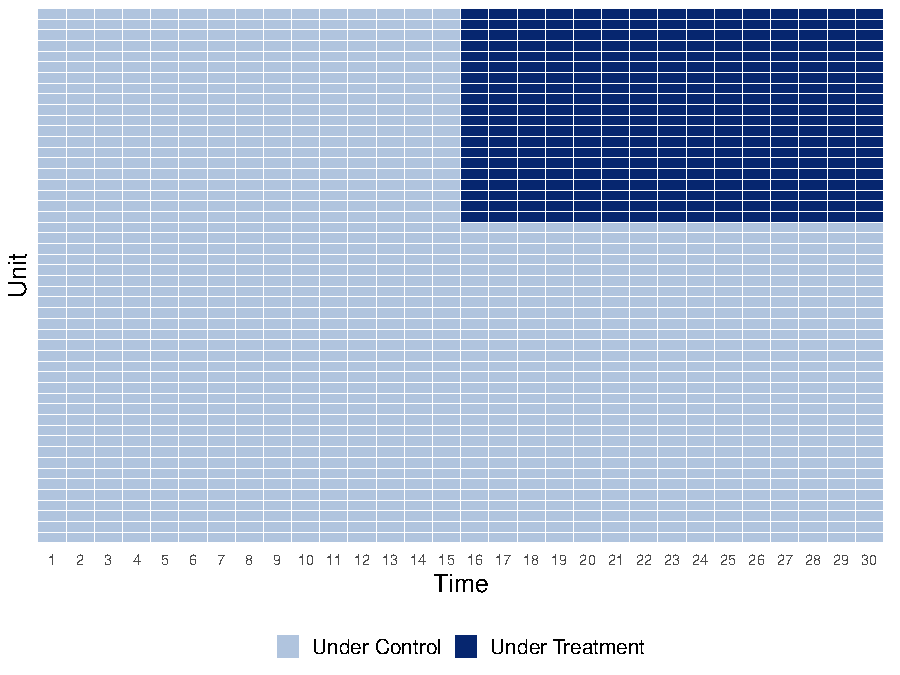
\includegraphics[width=\linewidth]{setting_block.pdf}
\end{column}
\begin{column}{0.32\textwidth}
\centering
\onslide<2->{\textbf{Staggered}\par\smallskip
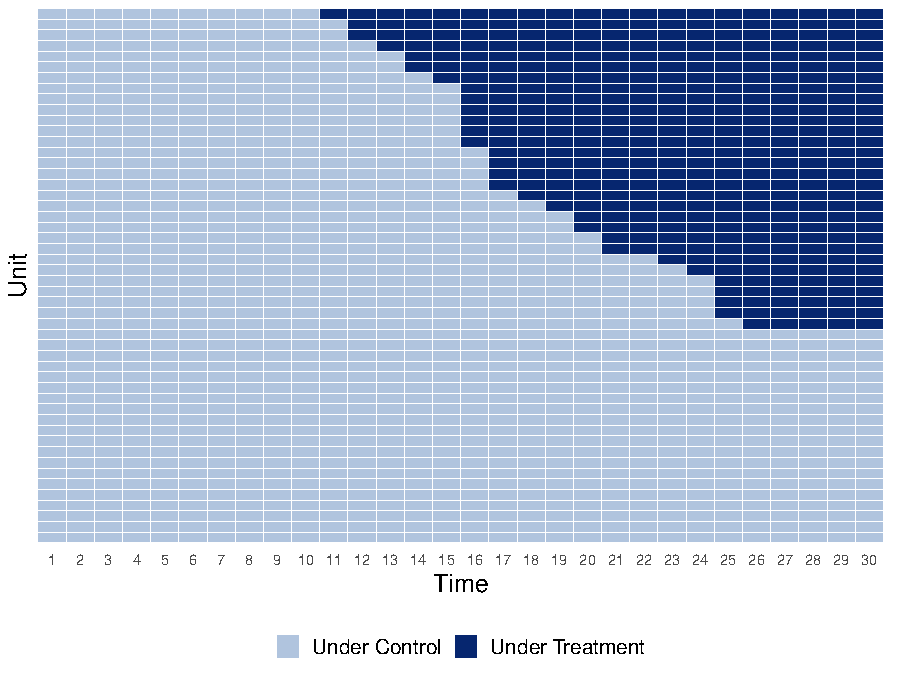
\includegraphics[width=\linewidth]{setting_staggered.pdf}}
\end{column}
\begin{column}{0.32\textwidth}
\centering
\onslide<3->{\textbf{General (w/ reversal)}\par\smallskip
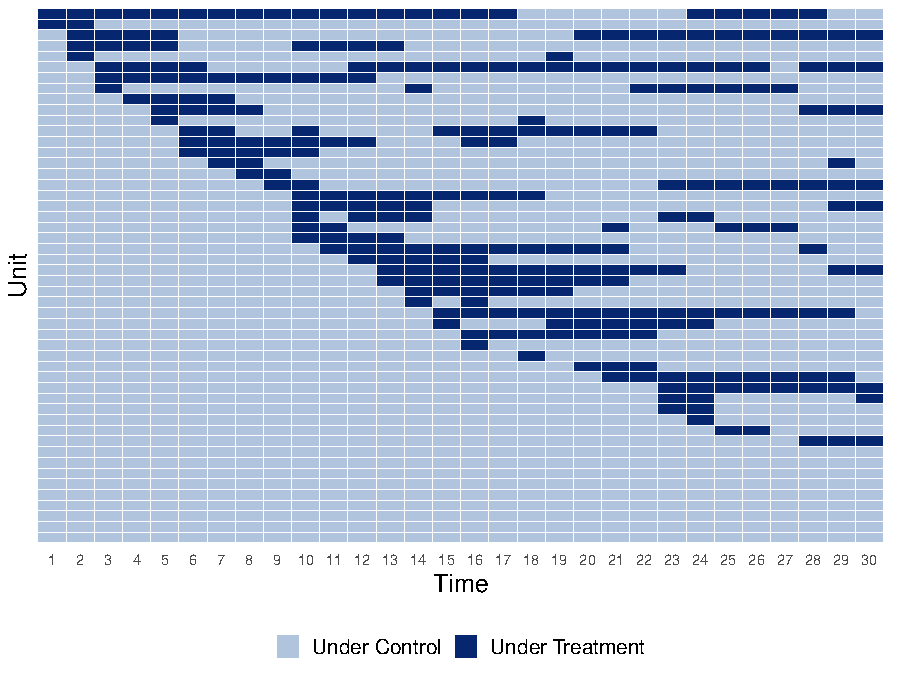
\includegraphics[width=\linewidth]{setting_general.pdf}}
\end{column}
\end{columns}
\bigskip
\begin{itemize}
\item<4-> Which estimators are available depends on the setting; treatment reversal (present in the majority of political science studies) rules out the staggered-only tools
\end{itemize}
\end{frame}

\begin{frame}
  \frametitle{The Organizing Principle}
\begin{center}
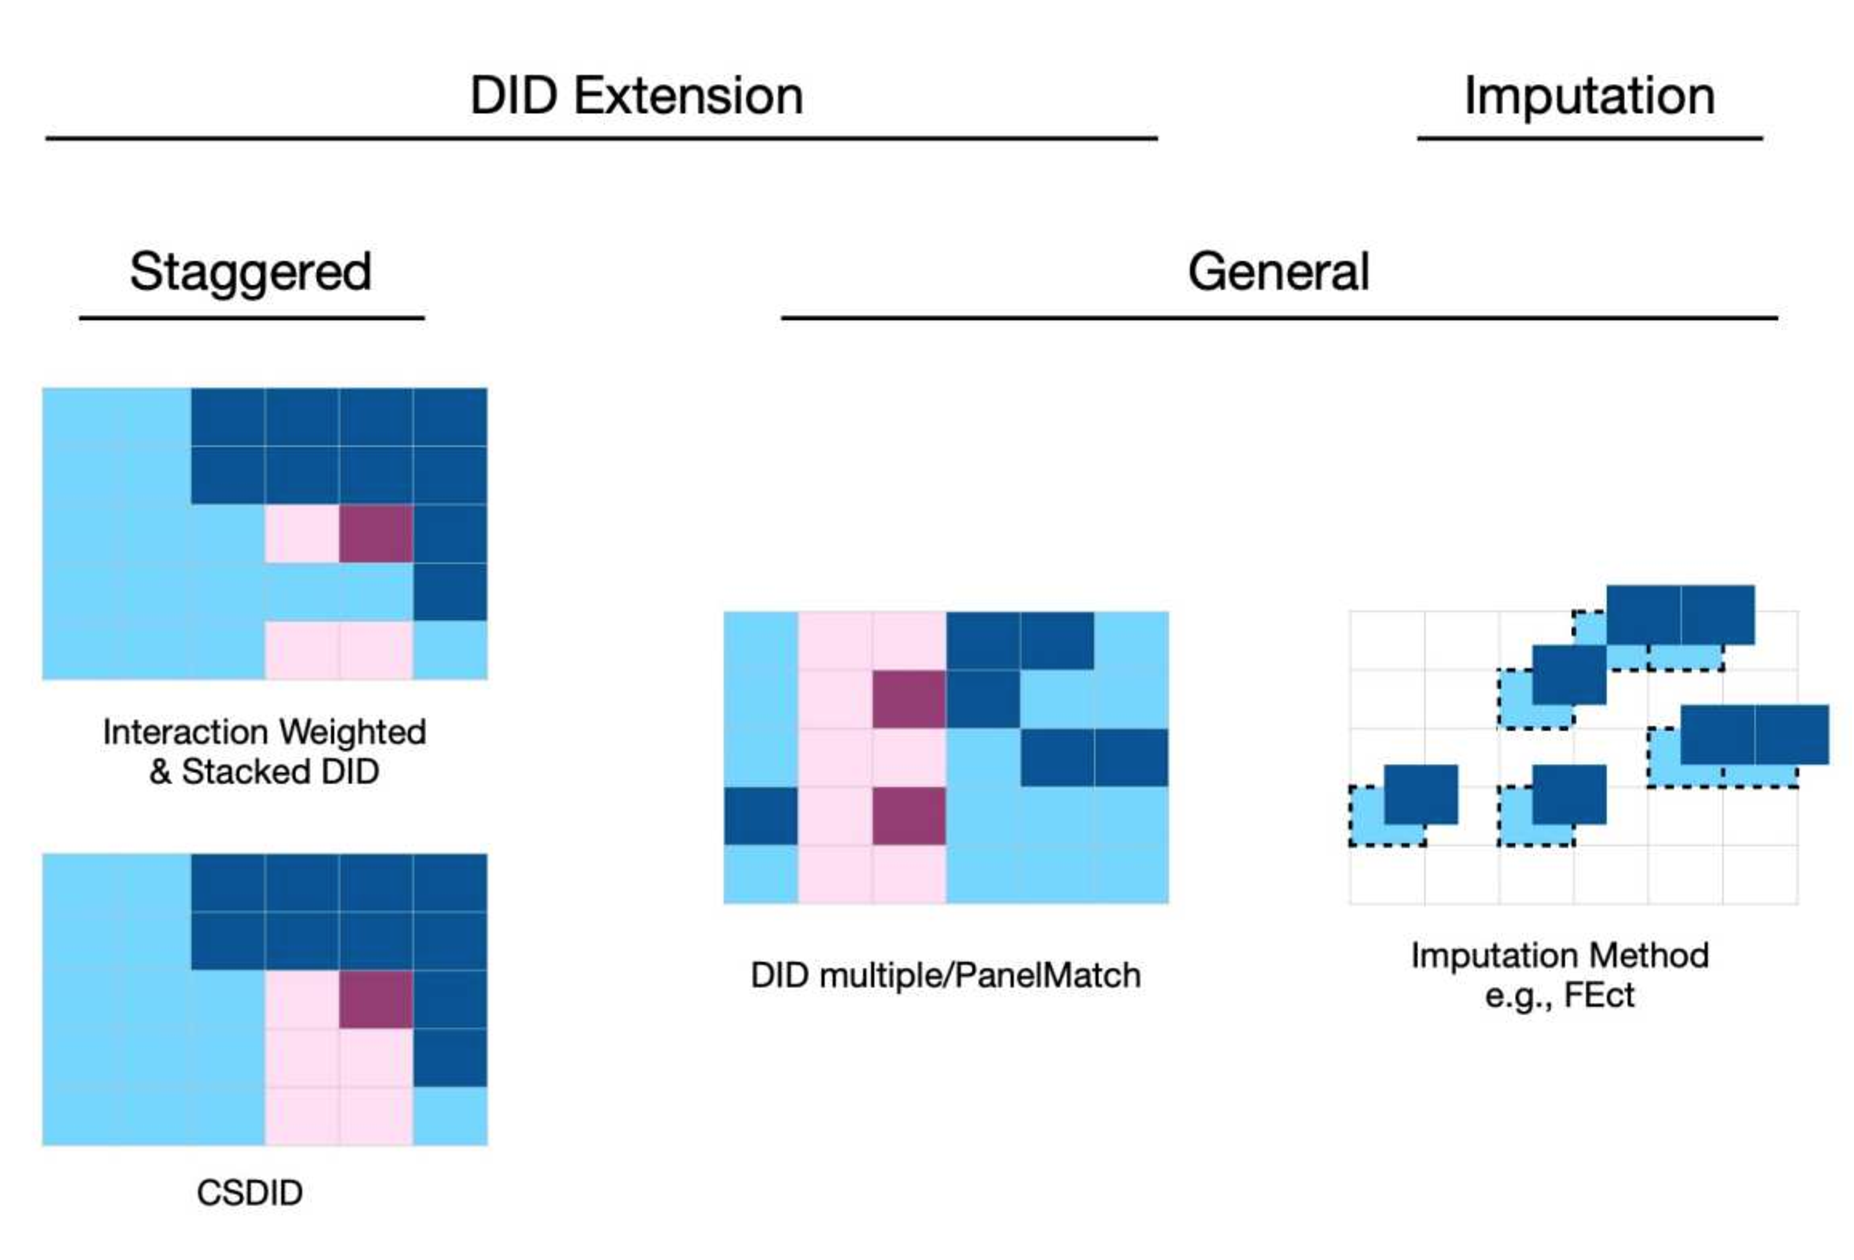
\includegraphics[width=0.78\textwidth, height=0.56\textheight, keepaspectratio]{hte_taxonomy.pdf}
\end{center}
\begin{itemize}
\item<2-> \alert{DID extensions} pick explicit $2\times 2$ comparisons; \alert{imputation methods} fit an outcome model on untreated cells only
\end{itemize}
\end{frame}

\begin{frame}[t]
  \frametitle{\textcite{sun2021estimating}: Interaction Weighted}
\begin{columns}[T,onlytextwidth]
\begin{column}{0.5\textwidth}
\begin{itemize}\itemsep0.8em
\item<2-> Comparison group: \alert{never-treated}
\item<3-> Estimate a cohort ATT (CATT) by $2\times 2$ DID for each cohort $g$ and period since treatment $l$
\item<6-> ATT $=$ average CATT, weighted by cohort size
\end{itemize}
\bigskip
\begin{itemize}
\item<3-> \only<3| handout:0>{\footnotesize CATT for cohort $\{A,B\}$ at $l=0$: compare the cohort with the never-treated across the reference and first treated periods}%
\only<4| handout:0>{\footnotesize The window sweeps forward for $l = 1, 2, 3$, always against the same reference period}%
\only<5-| handout:1>{\footnotesize The same construction for every cohort; shown here: cohort $C$ at $l=0$, the red window pairing the reference period with the first treated period}
\end{itemize}
\end{column}
\begin{column}{0.48\textwidth}
\centering
\begin{tikzpicture}[scale=0.9]
\useasboundingbox (-0.8,-1.6) rectangle (6.2,5.5);
\basegrid
% cohort {A,B} (g=3) highlighted with never-treated E
\only<3-4| handout:0>{%
  \foreach \c in {1,2} {\gcell{\c}{1}{cellP}\gcell{\c}{2}{cellP}}
  \foreach \c in {3,...,6} {\gcell{\c}{1}{cellG}\gcell{\c}{2}{cellG}}
  \foreach \c in {1,...,6} {\gcell{\c}{5}{cellP}}}
% cohort C (g=5)
\only<5-| handout:1>{%
  \foreach \c in {1,...,4} {\gcell{\c}{3}{cellP}}
  \foreach \c in {5,6} {\gcell{\c}{3}{cellG}}
  \foreach \c in {1,...,6} {\gcell{\c}{5}{cellP}}}
\gridframe
% sweeping comparison windows (reference column + post column)
\only<3| handout:0>{\draw[red, very thick] (1,-0.25) rectangle (2,5.25);
         \draw[red, very thick] (2,-0.25) rectangle (3,5.25);}
\only<4| handout:0>{\draw[red, very thick] (1,-0.25) rectangle (2,5.25);
         \draw[red, very thick] (5,-0.25) rectangle (6,5.25);}
\only<5-| handout:1>{\draw[red, very thick] (3,-0.4) rectangle (4,5.4);
         \draw[red, very thick] (4,-0.4) rectangle (5,5.4);}
\end{tikzpicture}
\end{column}
\end{columns}
\end{frame}

\begin{frame}
  \frametitle{Group-Time Effects and How to Aggregate Them}
\begin{itemize}[<+->]\itemsep0.9em
\item The building block behind these estimators is the \alert{group-time ATT}:
\begin{equation*}
ATT(g, t) = \E[Y_{it}(1) - Y_{it}(0) \mid G_i = g], \qquad t \geq g
\end{equation*}
the effect for the cohort first treated at $g$, in calendar period $t$
\item One number per cohort-period pair is too much detail; the art is in the \alert{aggregation}:
\begin{itemize}\itemsep0.5em
  \item By relative time $l = t - g$: the \alert{event-study} plot
  \item By calendar time $t$: does the effect grow or fade over the sample period?
  \item Overall: a weighted average across all treated cohort-periods
\end{itemize}
\item Different papers need different aggregations; report the one your theory speaks to, not just the overall number
\end{itemize}
\end{frame}

\begin{frame}[t]
  \frametitle{\textcite{callaway2021difference}}
\begin{itemize}\itemsep0.5em
\item Comparison group: \alert{not-yet-treated} (in addition to never-treated)
\item<3-> ``Doubly robust'' with covariates: combines outcome regression and propensity-score weighting
\end{itemize}
\medskip
\begin{columns}[T,onlytextwidth]
\begin{column}{0.48\textwidth}
\centering
\textbf{\textcite{sun2021estimating}}\par\medskip
\begin{tikzpicture}[scale=0.6]
\basegrid
\foreach \c in {1,...,4} {\gcell{\c}{3}{cellP}}
\gcell{5}{3}{cellG}
\foreach \c in {1,...,6} {\gcell{\c}{5}{cellP}}
\gridframe
\end{tikzpicture}
\end{column}
\begin{column}{0.48\textwidth}
\centering
\onslide<2->{\textbf{\textcite{callaway2021difference}}\par\medskip
\begin{tikzpicture}[scale=0.6]
\basegrid
\foreach \c in {1,...,4} {\gcell{\c}{3}{cellP}}
\gcell{5}{3}{cellG}
\foreach \c in {1,...,5} {\gcell{\c}{4}{cellP}}
\foreach \c in {1,...,6} {\gcell{\c}{5}{cellP}}
\gridframe
\end{tikzpicture}}
\end{column}
\end{columns}
\medskip
\begin{itemize}
\item<4-> More comparison cells $\Rightarrow$ more power, at the price of assuming parallel trends also holds for the not-yet-treated
\end{itemize}
\end{frame}

\begin{frame}[t]
  \frametitle{Stacked DID (\cite{cengiz2019effect})}
\begin{itemize}\itemsep0.4em
\item<1-> Build one dataset per cohort: the cohort's units plus \alert{a copy of the pure comparison group}, the never-treated $E$
\item<2-> ``Stack'' the cohort datasets and re-index time relative to each cohort's onset, so that the switches line up
\item<3-> One saturated regression on the stack, with unit and period effects specific to each dataset; similar to interaction weighting, but with disproportionate weights across cohorts
\end{itemize}
\begin{center}
\begin{tikzpicture}[scale=0.37]
\useasboundingbox (-1.2,-5.0) rectangle (29.5,5.4);
% stage 1: the staggered data
\basegrid \gridframe
\node[below=13pt] at (3,0) {\scriptsize original data};
% stage 2: one dataset per cohort, each with its own copy of E
\begin{scope}[xshift=9.5cm]
\only<2->{%
\cblock{0}{2}{2}{3} \cblock{0}{-0.5}{1}{5} \cblock{0}{-3}{1}{6}
\foreach \y/\l in {4.5/A,3.5/B,2.5/E,1/C,0/E,-1.5/D,-2.5/E} {\node[left=2pt] at (0,\y) {\small \l};}
\foreach \c in {1,...,6} {\node[below=2pt] at ({\c-0.5},-3) {\small \c};}
\node[below=13pt] at (3,-3) {\scriptsize one dataset per cohort};}
\end{scope}
% stage 3: the same blocks, shifted so the onsets align
\begin{scope}[xshift=19.5cm]
\only<3->{%
\cblock{3}{2}{2}{3} \cblock{1}{-0.5}{1}{5} \cblock{0}{-3}{1}{6}
\foreach \y/\l/\x in {4.5/A/3,3.5/B/3,2.5/E/3,1/C/1,0/E/1,-1.5/D/0,-2.5/E/0} {\node[left=2pt] at (\x,\y) {\small \l};}
\draw[red, thick, dashed] (5,-3.3) -- (5,5.3);
\foreach \c/\l in {1/{$-5$},2/{$-4$},3/{$-3$},4/{$-2$},5/{$-1$},6/{$0$},7/{$1$},8/{$2$},9/{$3$}} {\node[below=2pt] at ({\c-0.5},-3) {\small \l};}
\node[below=13pt] at (4.5,-3) {\scriptsize stacked and aligned on event time $l$};}
\end{scope}
\end{tikzpicture}
\end{center}
\vspace{-1em}
{\scriptsize In practice a unit serves as a comparison for a cohort only while it stays untreated inside that cohort's event window (``clean controls'').}
\end{frame}

\begin{frame}[t]
  \frametitle{\textcite{dechaisemartin2020twoway}: DID\texorpdfstring{$_M$}{M}}
\begin{columns}[T,onlytextwidth]
\begin{column}{0.52\textwidth}
\begin{itemize}\itemsep0.55em
\item<1-> No cohorts: one average effect \alert{for switchers}, not the ATT; works with treatment reversal
\item<2-> Switchers: $(i,t)$ with $D_{it} \neq D_{i,t-1}$; \only<2-| handout:1->{here $B$ and $D$ at period 3}
\item<3-> Stable group: $(i,t)$ with $D_{it} = D_{i,t-1}$, sharing the switchers' status in the previous period; \only<3-| handout:1->{here $A$, $C$, $E$}
\item<4-> DID$_M$: a DID from period 2 to 3, switchers against the stable group, estimates the \alert{contemporaneous} effect at the period of the switch; leavers ($1 \to 0$) are compared with stable treated units in the same way, with the sign reversed
\item<5-> Same data as PanelMatch on the next page: DID$_M$ is PanelMatch with $a = l = 1$ and no refinement
\end{itemize}
\end{column}
\begin{column}{0.46\textwidth}
\centering
\begin{tikzpicture}[scale=0.85]
\useasboundingbox (-0.8,-1.0) rectangle (6.2,5.3);
\generalgrid
\only<4-| handout:1>{%
  \foreach \r in {1,3,5} {\gcell{2}{\r}{cellP}\gcell{3}{\r}{cellP}}
  \gcell{2}{2}{cellP}\gcell{3}{2}{cellG}
  \gcell{2}{4}{cellP}\gcell{3}{4}{cellG}}
\gridframerows
\foreach \c/\l in {2/{$0$},3/{$1$}} {\node[below=2pt] at ({\c-0.5},0) {\small \l};}
\only<2| handout:0>{\draw[red, very thick] (1,3) rectangle (3,4); \draw[red, very thick] (1,1) rectangle (3,2);}
\only<3| handout:0>{\draw[red, very thick] (1,4) rectangle (3,5); \draw[red, very thick] (1,2) rectangle (3,3); \draw[red, very thick] (1,0) rectangle (3,1);}
\only<4| handout:0>{\draw[red, very thick] (1,-0.3) rectangle (3,5.3);}
\end{tikzpicture}
\end{column}
\end{columns}
\end{frame}

\begin{frame}[t]
  \frametitle{PanelMatch (\cite{imai2023matching})}
\begin{columns}[T,onlytextwidth]
\begin{column}{0.52\textwidth}
\begin{itemize}\itemsep0.45em
\item<1-> General setting: match each treated $(i,t)$ to units with the \alert{same treatment history} over the previous $a$ periods
\item<2-> $a = 2$: for $B$ at period 3 the matched set is $\{A, C, E\}$, untreated in periods 1--2 like $B$; \only<3-| handout:1->{$D$ (treated in period 1) is \alert{excluded}}
\item<4-> A DID from period 2 to 3 within the matched set: the effect at $l = 1$
\item<5-> Later periods $l = 2, 3, \ldots$ (up to reversal): units that switch inside the window drop out; here $A$ leaves at $l = 2$
\item<6-> Refine the matched set on covariates $X_{it}$
\item<7-> DID$_M$: the case $a = l = 1$ without refinement; at period 3 the switchers $B$ and $D$ are matched to $A$, $C$, $E$
\end{itemize}
\end{column}
\begin{column}{0.46\textwidth}
\centering
{\small \only<1-4| handout:1>{e.g., $a = 2$}\only<5-6| handout:2>{e.g., $l = 2$}\only<7| handout:3>{DID$_M$: $a = l = 1$}}\par\smallskip
\begin{tikzpicture}[scale=0.85]
\useasboundingbox (-0.8,-1.0) rectangle (6.2,5.3);
\generalgrid
\only<2-4| handout:1>{%
  \foreach \c in {1,2,3} {\gcell{\c}{1}{cellP}\gcell{\c}{3}{cellP}\gcell{\c}{5}{cellP}}
  \gcell{1}{2}{cellP}\gcell{2}{2}{cellP}\gcell{3}{2}{cellG}}
\only<5-6| handout:2>{%
  \foreach \c in {1,2,3,4} {\gcell{\c}{3}{cellP}\gcell{\c}{5}{cellP}}
  \gcell{1}{2}{cellP}\gcell{2}{2}{cellP}\gcell{3}{2}{cellG}\gcell{4}{2}{cellG}}
\only<7| handout:3>{%
  \foreach \r in {1,3,5} {\gcell{2}{\r}{cellP}\gcell{3}{\r}{cellP}}
  \gcell{2}{2}{cellP}\gcell{3}{2}{cellG}
  \gcell{2}{4}{cellP}\gcell{3}{4}{cellG}}
\gridframerows
\only<1-4| handout:1>{\foreach \c/\l in {1/{$-1$},2/{$0$},3/{$1$}} {\node[below=2pt] at ({\c-0.5},0) {\small \l};}}
\only<5-7| handout:2-3>{\foreach \c/\l in {1/{$-1$},2/{$0$},3/{$1$},4/{$2$}} {\node[below=2pt] at ({\c-0.5},0) {\small \l};}}
\only<3| handout:0>{\draw[red, very thick] (0,1) rectangle (3,2);
  \draw[red, very thick, -{Latex[length=2mm]}] (2.3,3.2) -- (1.6,2.25);}
\only<4| handout:0>{\draw[red, very thick] (1,-0.3) rectangle (3,5.3);}
\end{tikzpicture}
\end{column}
\end{columns}
\end{frame}

\begin{frame}[t]
  \frametitle{Imputation Methods (\citeshort{borusyak2021revisiting}; \cite{liu2024practical})}
\begin{columns}[T,onlytextwidth]
\begin{column}{0.52\textwidth}
\begin{itemize}\itemsep0.6em
\item<1-> Also for the general setting, with a different logic: model the untreated outcome instead of choosing comparisons
\item<2-> Set the treated cells aside and fit a model for $Y_{it}(0)$ on the \alert{untreated cells only}; with two-way fixed effects, this is the fixed effects counterfactual estimator (FEct)
\item<3-> Impute $\hat{Y}_{it}(0)$ for every treated cell
\item<4-> One estimate per treated cell: $\hat{\delta}_{it} = Y_{it} - \hat{Y}_{it}(0)$
\item<5-> Summarize the $\hat{\delta}_{it}$ however the question demands: overall ATT, dynamic effects, subgroups; no forbidden comparisons by construction; efficient under homoskedasticity \parenciteshort{borusyak2021revisiting}
\end{itemize}
\end{column}
\begin{column}{0.46\textwidth}
\centering
\begin{tikzpicture}[scale=0.85]
\useasboundingbox (-0.8,-1.3) rectangle (6.5,5.6);
\only<1| handout:0>{\generalgrid}
\only<2-| handout:1->{\fill[cellC] (0,0) rectangle (6,5);
  \foreach \c/\r in {4/1,5/1,3/2,4/2,5/3,6/3,1/4,3/4} {\gcell{\c}{\r}{white}}}
\gridframerows
\foreach \c in {1,...,6} {\node[below=2pt] at ({\c-0.5},0) {\small \c};}
\only<3-| handout:1->{\foreach \c/\r in {4/1,5/1,3/2,4/2,5/3,6/3,1/4,3/4} {\draw[cellT, densely dashed, thick] ({\c-1+0.07},{5-\r+0.07}) rectangle ({\c-0.07},{6-\r-0.07});}}
\only<4-| handout:2>{\foreach \c/\r in {4/1,5/1,3/2,4/2,5/3,6/3,1/4,3/4} {\fill[cellT] ({\c-1+0.28},{5-\r+0.28}) rectangle ({\c+0.28},{6-\r+0.28});}}
\node[below=14pt, text width=5.6cm, align=center] at (3,0) {\scriptsize \only<1| handout:0>{dark: treated cells; light: untreated cells}\only<2| handout:0>{treated cells set aside; the model is fit on what remains}\only<3| handout:1>{dashed: the imputed $\hat{Y}_{it}(0)$ for each treated cell}\only<4-| handout:2>{observed $Y_{it}$ (solid) over imputed $\hat{Y}_{it}(0)$ (dashed): $\hat{\delta}_{it}$}};
\end{tikzpicture}
\end{column}
\end{columns}
\end{frame}

\begin{frame}[t]
  \frametitle{Extended TWFE, or the Two-Way Mundlak Regression (\cite{wooldridge2025twoway})}
\begin{itemize}\itemsep0.55em
\item<1-> Keep the regression, but let the effect differ by cohort and period: one coefficient $\tau_{gt}$ for every cohort $g$ in every post-treatment period $t \geq g$, instead of a single $\tau$
\begin{equation*}
Y_{it} = \alpha_i + \xi_t + \sum_{g} \sum_{t' \geq g} \tau_{gt'}\, \mathbf{1}\{G_i = g\}\, \mathbf{1}\{t = t'\} + \varepsilon_{it}
\end{equation*}
\item<2-> ``Mundlak'': in a balanced panel, replacing the unit effects by cohort dummies (the unit-level means of the regressors) gives numerically the same $\hat{\tau}_{gt}$, so the whole thing is one pooled regression
\item<3-> Which cells compare: with no pre-period dummies, every pre-treatment cell stays in the untreated pool that pins down $\alpha_i$ and $\xi_t$, exactly as in imputation (IW and CSDID instead compare against one reference period); in a balanced panel without covariates the $\hat{\tau}_{gt}$ equal the imputation estimates
\item<4-> Why it has caught on: one regression command with regression standard errors; covariates enter interacted with cohort and period; the same device extends to \alert{nonlinear models} (Poisson for counts, logit for binary outcomes; \cite{wooldridge2023simple}), where subtracting an imputed $\hat{Y}(0)$ makes no sense
\item<5-> Limits: staggered adoption only (a cohort is a first-treatment date, so no reversal); many coefficients, to be aggregated as with CSDID; parallel trends still does the identifying work. Software: \texttt{etwfe} (R), \texttt{jwdid} (Stata)
\end{itemize}
\end{frame}

\begin{frame}
  \frametitle{The Estimators, Side by Side}
\begin{center}
\renewcommand{\arraystretch}{1.75}
\small
\begin{tabular}{lcccc}
 & \multicolumn{2}{c}{\textbf{DID extensions}} & \multicolumn{2}{c}{\textbf{Imputation methods}} \\
 & \multicolumn{2}{c}{\footnotesize ($2\times2$ DIDs as building blocks)} & \multicolumn{2}{c}{\footnotesize (outcome model w/ FE)} \\ \hline
Setting & Staggered & General & Staggered & General \\
Estimand & ATT & ATT for switchers & ATT by cohort-period & ATT \\
Estimator & IW, CSDID, stacked & PanelMatch, DID$_M$ & \makecell{extended TWFE\\(two-way Mundlak)} & BJS, FEct \\
Comparisons & \makecell{never/not-yet-\\treated} & matched set & \makecell{imputed counterfactual,\\one saturated regression} & \makecell{imputed\\counterfactual} \\
Pre-treatment info & one reference period & the $a$ previous periods & all untreated cells & all untreated cells \\
Key assumption & parallel trends & parallel trends & \makecell{zero conditional mean\\or parallel trends} & \makecell{zero conditional mean\\or parallel trends} \\ \hline
\end{tabular}
\end{center}
\end{frame}

\begin{frame}
  \frametitle{Which Estimator Should I Use?}
\begin{itemize}[<+->]\itemsep1em
\item \textbf{Two-period or block assignment}: canonical DID is fine; TWFE equals DID here
\item \textbf{Staggered, no reversal}: the full menu applies; IW/CSDID if cohort effects are the object, imputation for flexibility and diagnostics; extended TWFE when the outcome calls for a nonlinear model
\item \textbf{Treatment reversal} (most political science panels): PanelMatch, DID$_M$, or imputation; the staggered-only tools do not apply
\item \textbf{Few treated units or one treated unit}: move to synthetic control territory (Lecture 6)
\item In well-powered data the choice rarely drives the answer; choose for \alert{diagnostics and transparency}, then show robustness across estimators
\end{itemize}
\end{frame}

\begin{frame}
  \frametitle{One Staggered Application, Five Estimators}
\begin{columns}[T,onlytextwidth]
\begin{column}{0.32\textwidth}
\centering
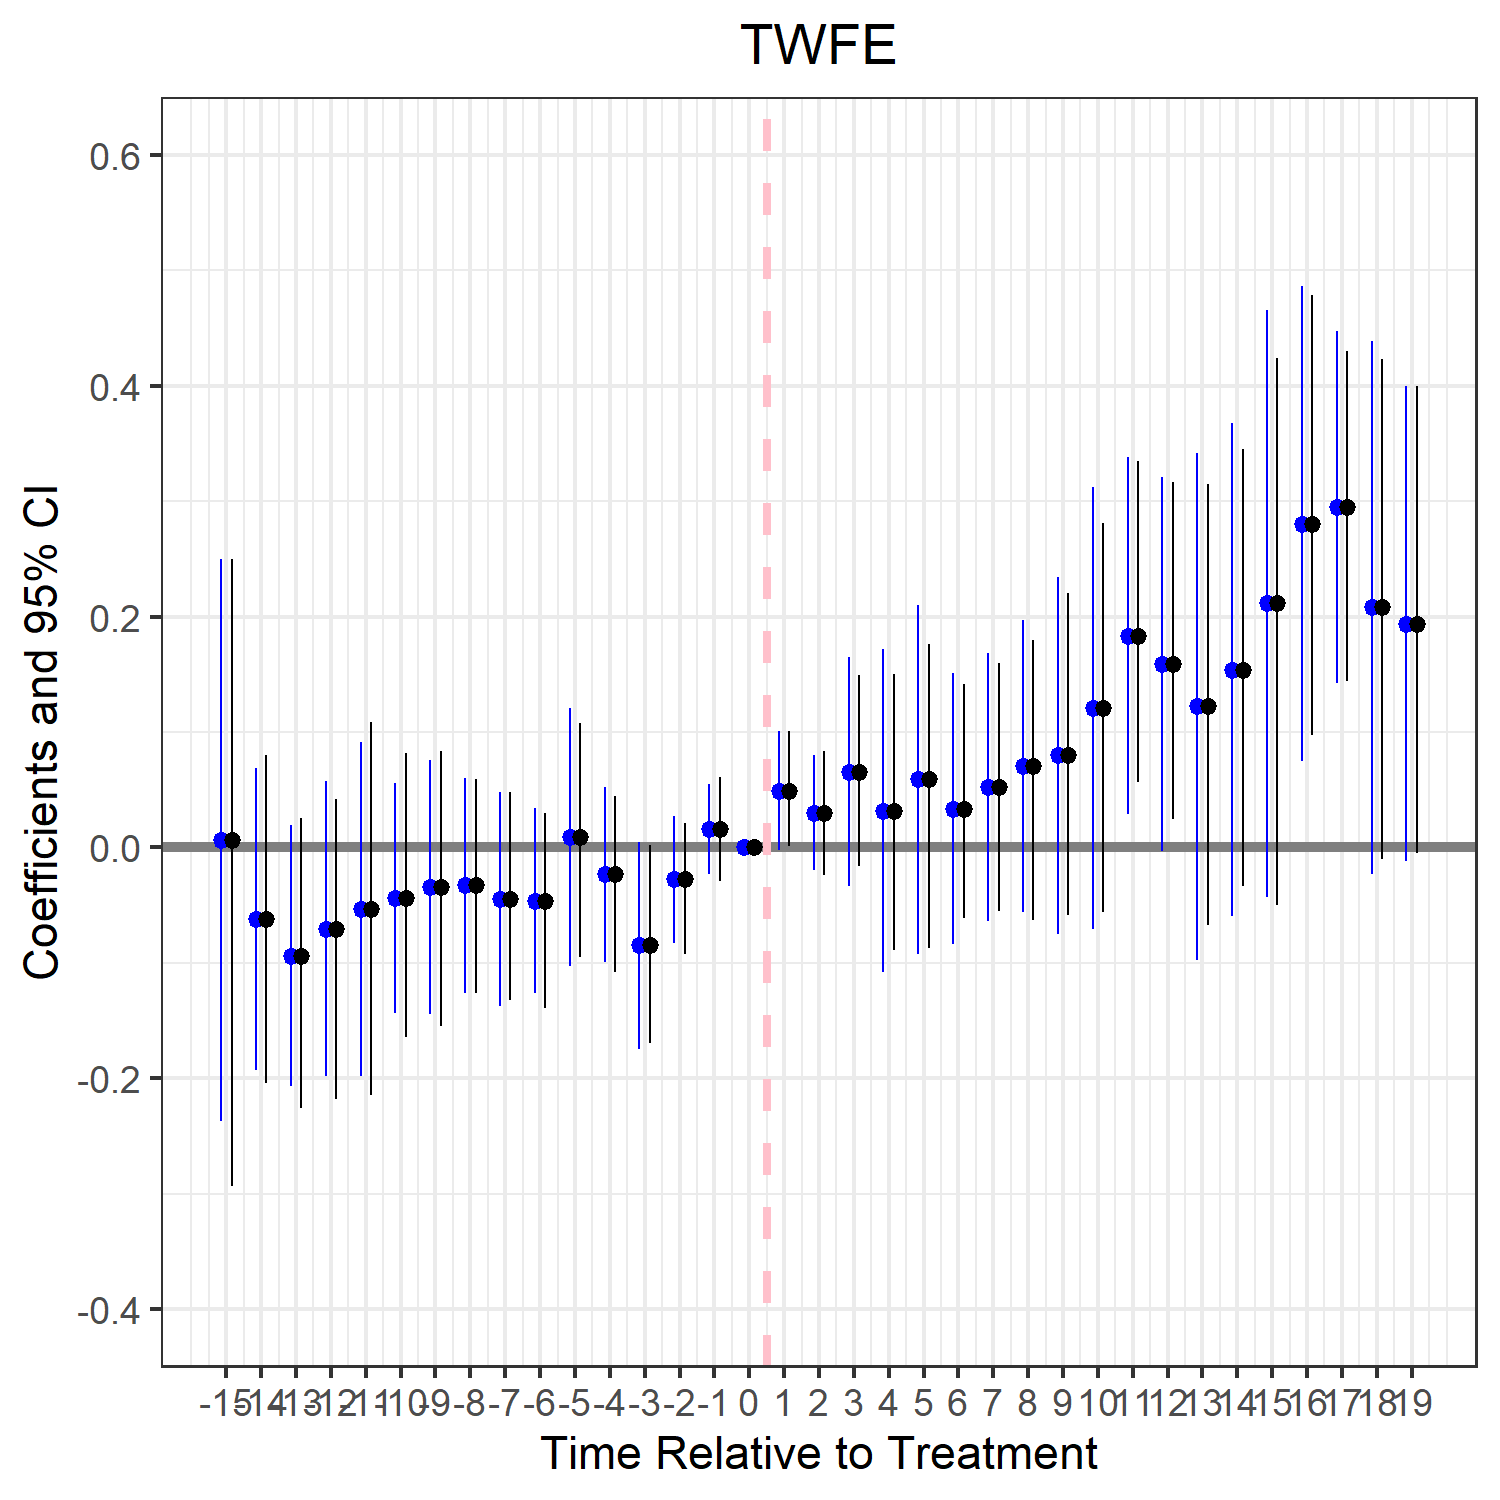
\includegraphics[width=\linewidth, height=0.27\textheight, keepaspectratio]{bischof_twfe.png}
\par{\scriptsize TWFE event study}
\end{column}
\begin{column}{0.32\textwidth}
\centering
\onslide<2->{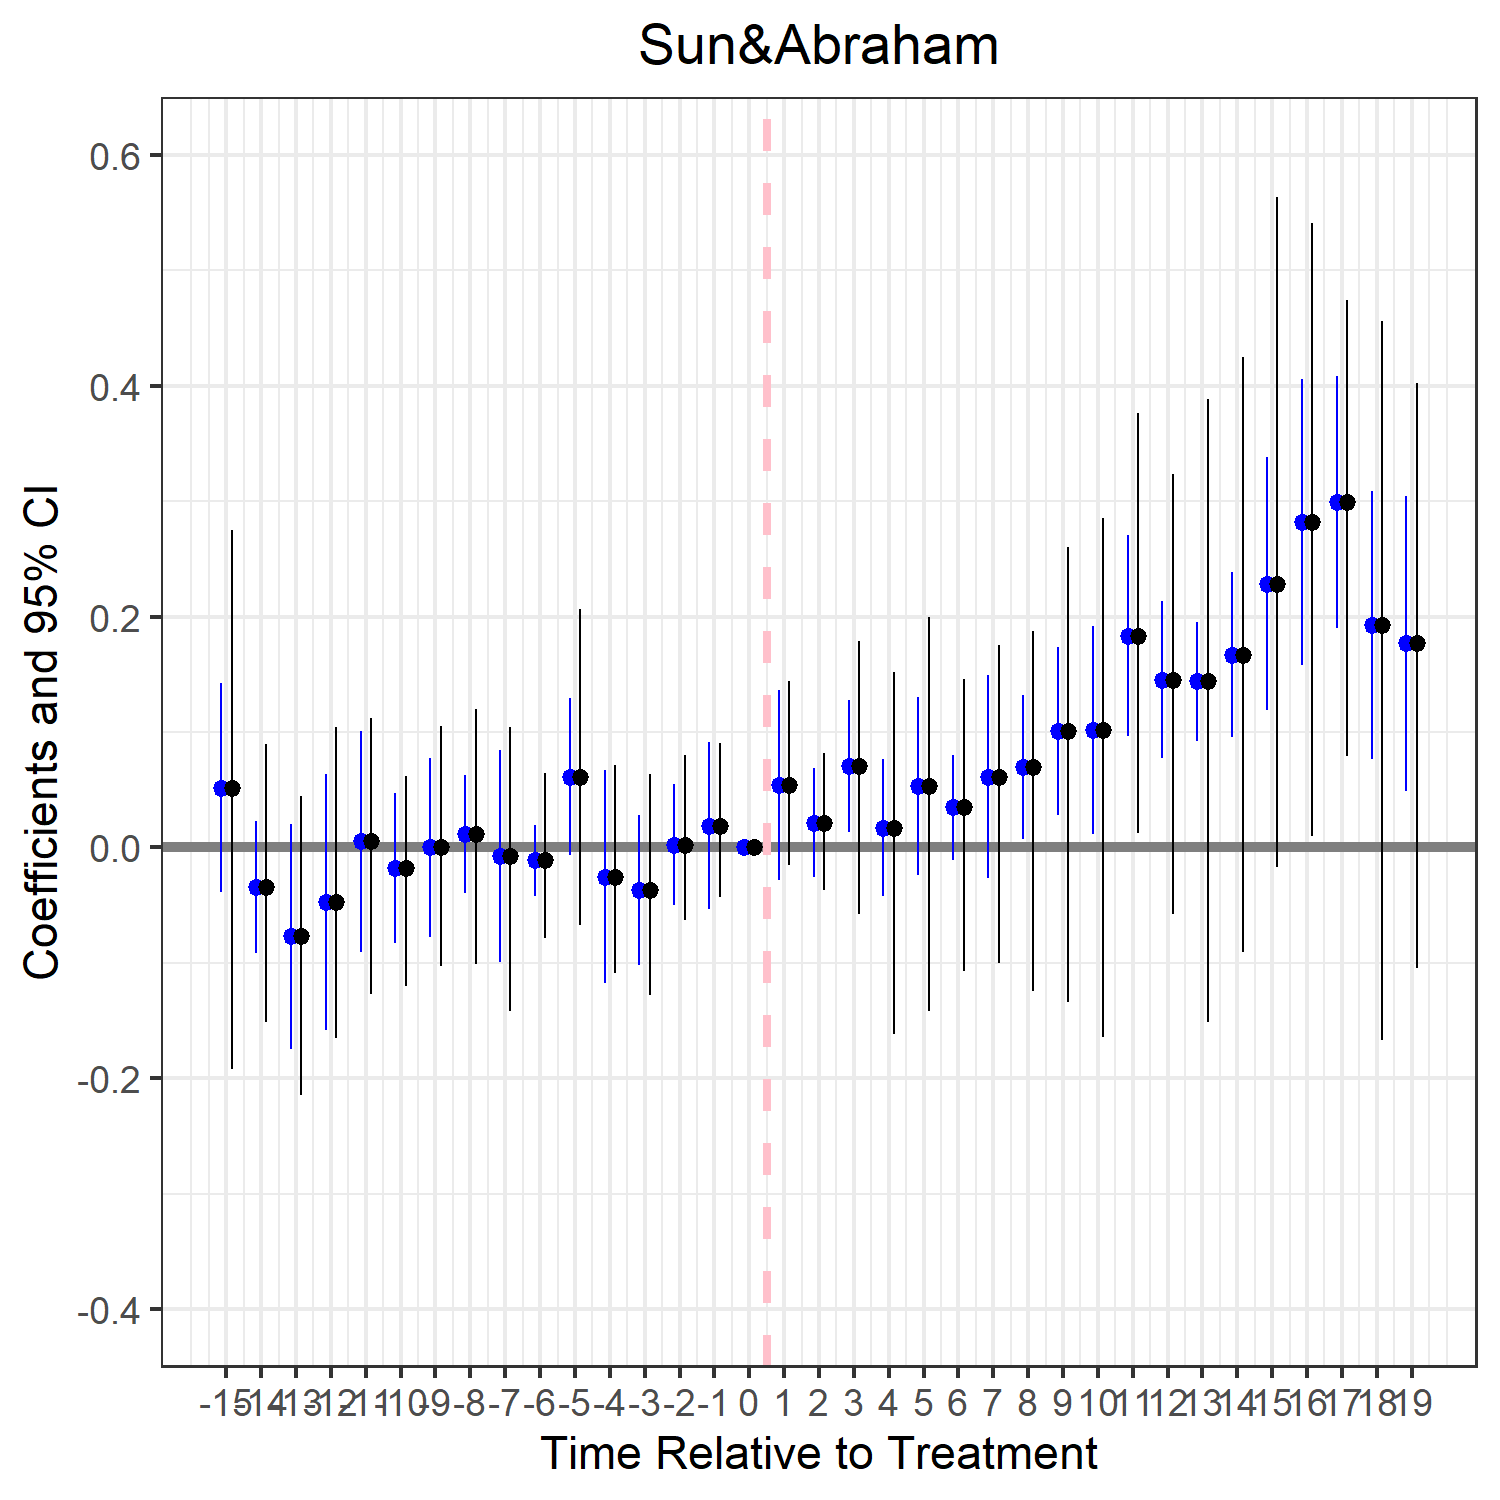
\includegraphics[width=\linewidth, height=0.27\textheight, keepaspectratio]{bischof_sa.png}
\par{\scriptsize Sun and Abraham}}
\end{column}
\begin{column}{0.32\textwidth}
\centering
\onslide<2->{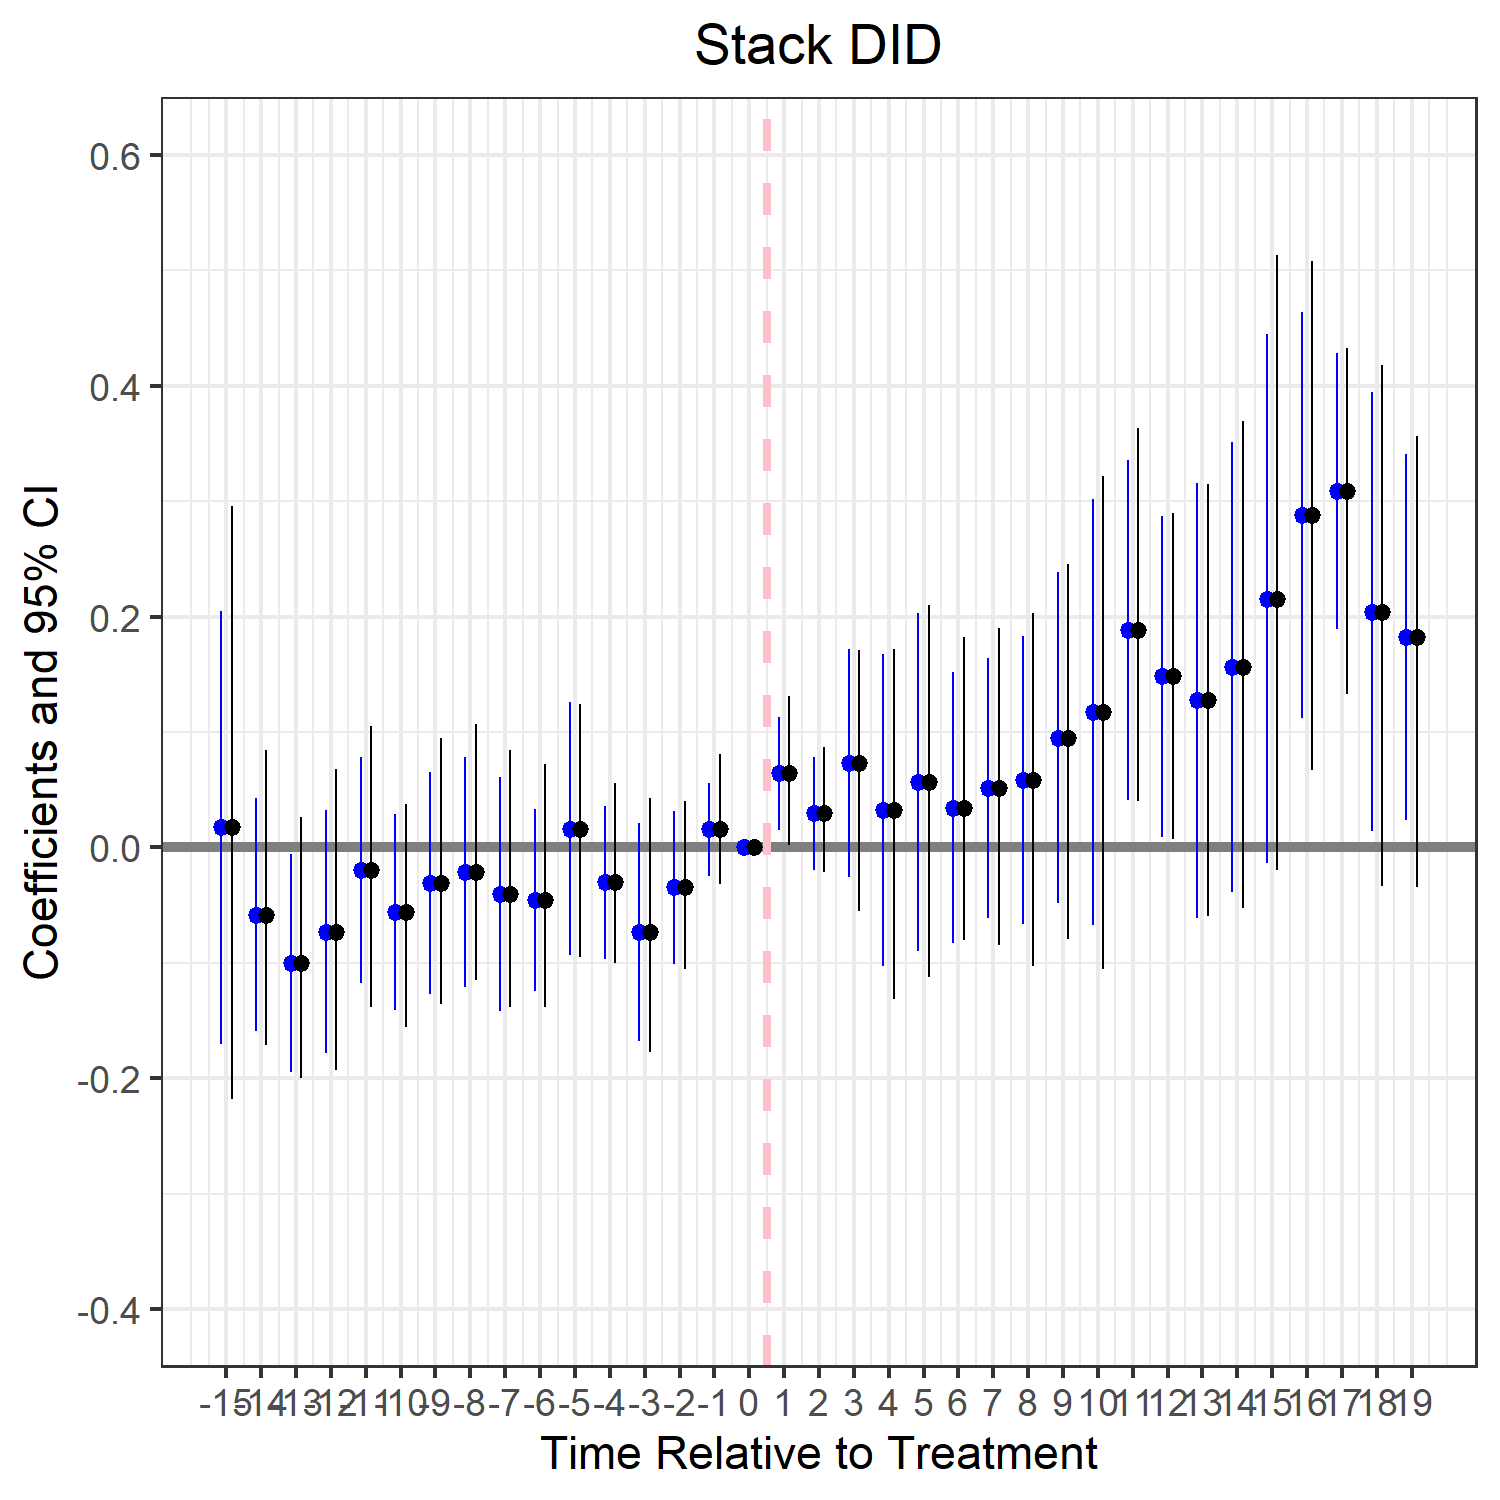
\includegraphics[width=\linewidth, height=0.27\textheight, keepaspectratio]{bischof_stack.png}
\par{\scriptsize stacked DID}}
\end{column}
\end{columns}
\medskip
\begin{columns}[T,onlytextwidth]
\begin{column}{0.32\textwidth}
\centering
\onslide<3->{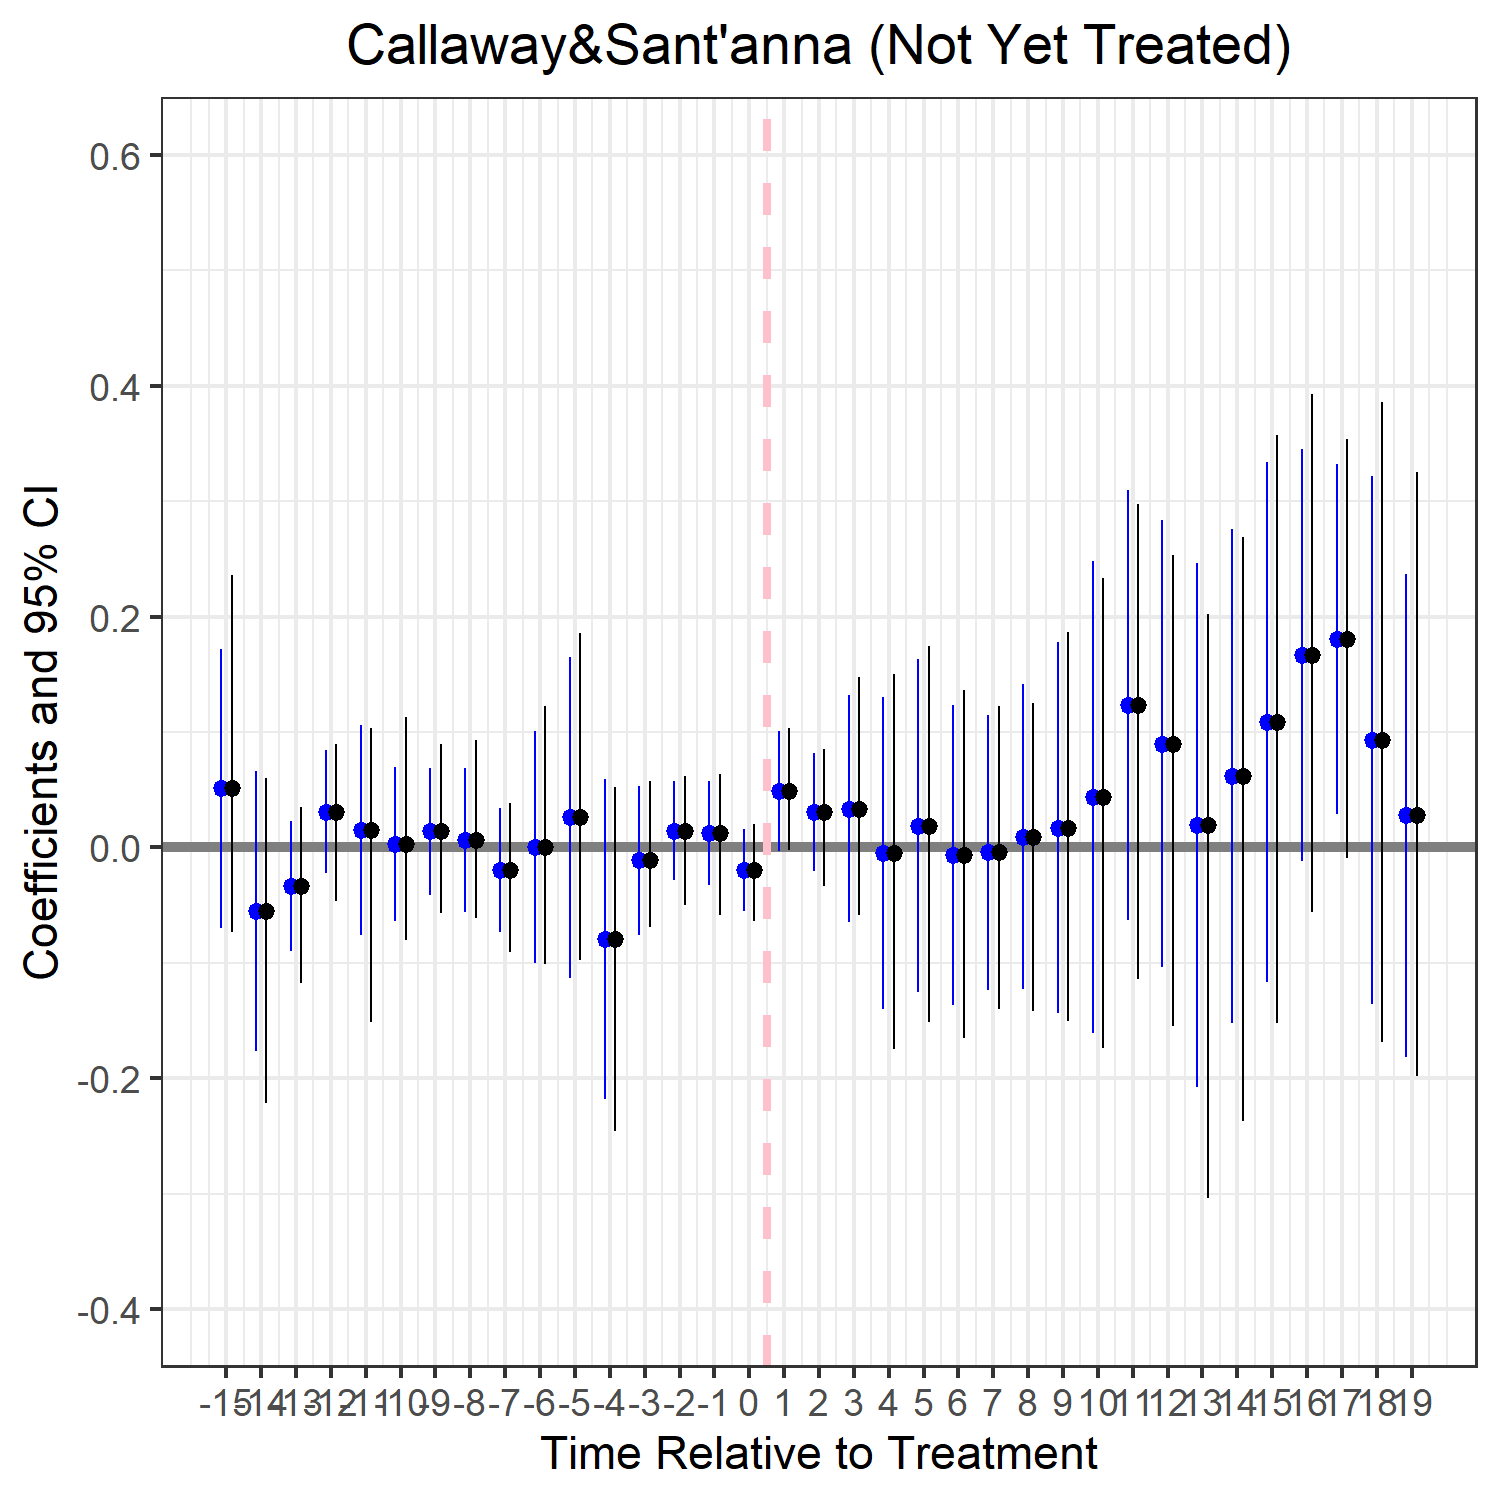
\includegraphics[width=\linewidth, height=0.27\textheight, keepaspectratio]{bischof_cs1.png}
\par{\scriptsize CSDID (not-yet-treated)}}
\end{column}
\begin{column}{0.32\textwidth}
\centering
\onslide<3->{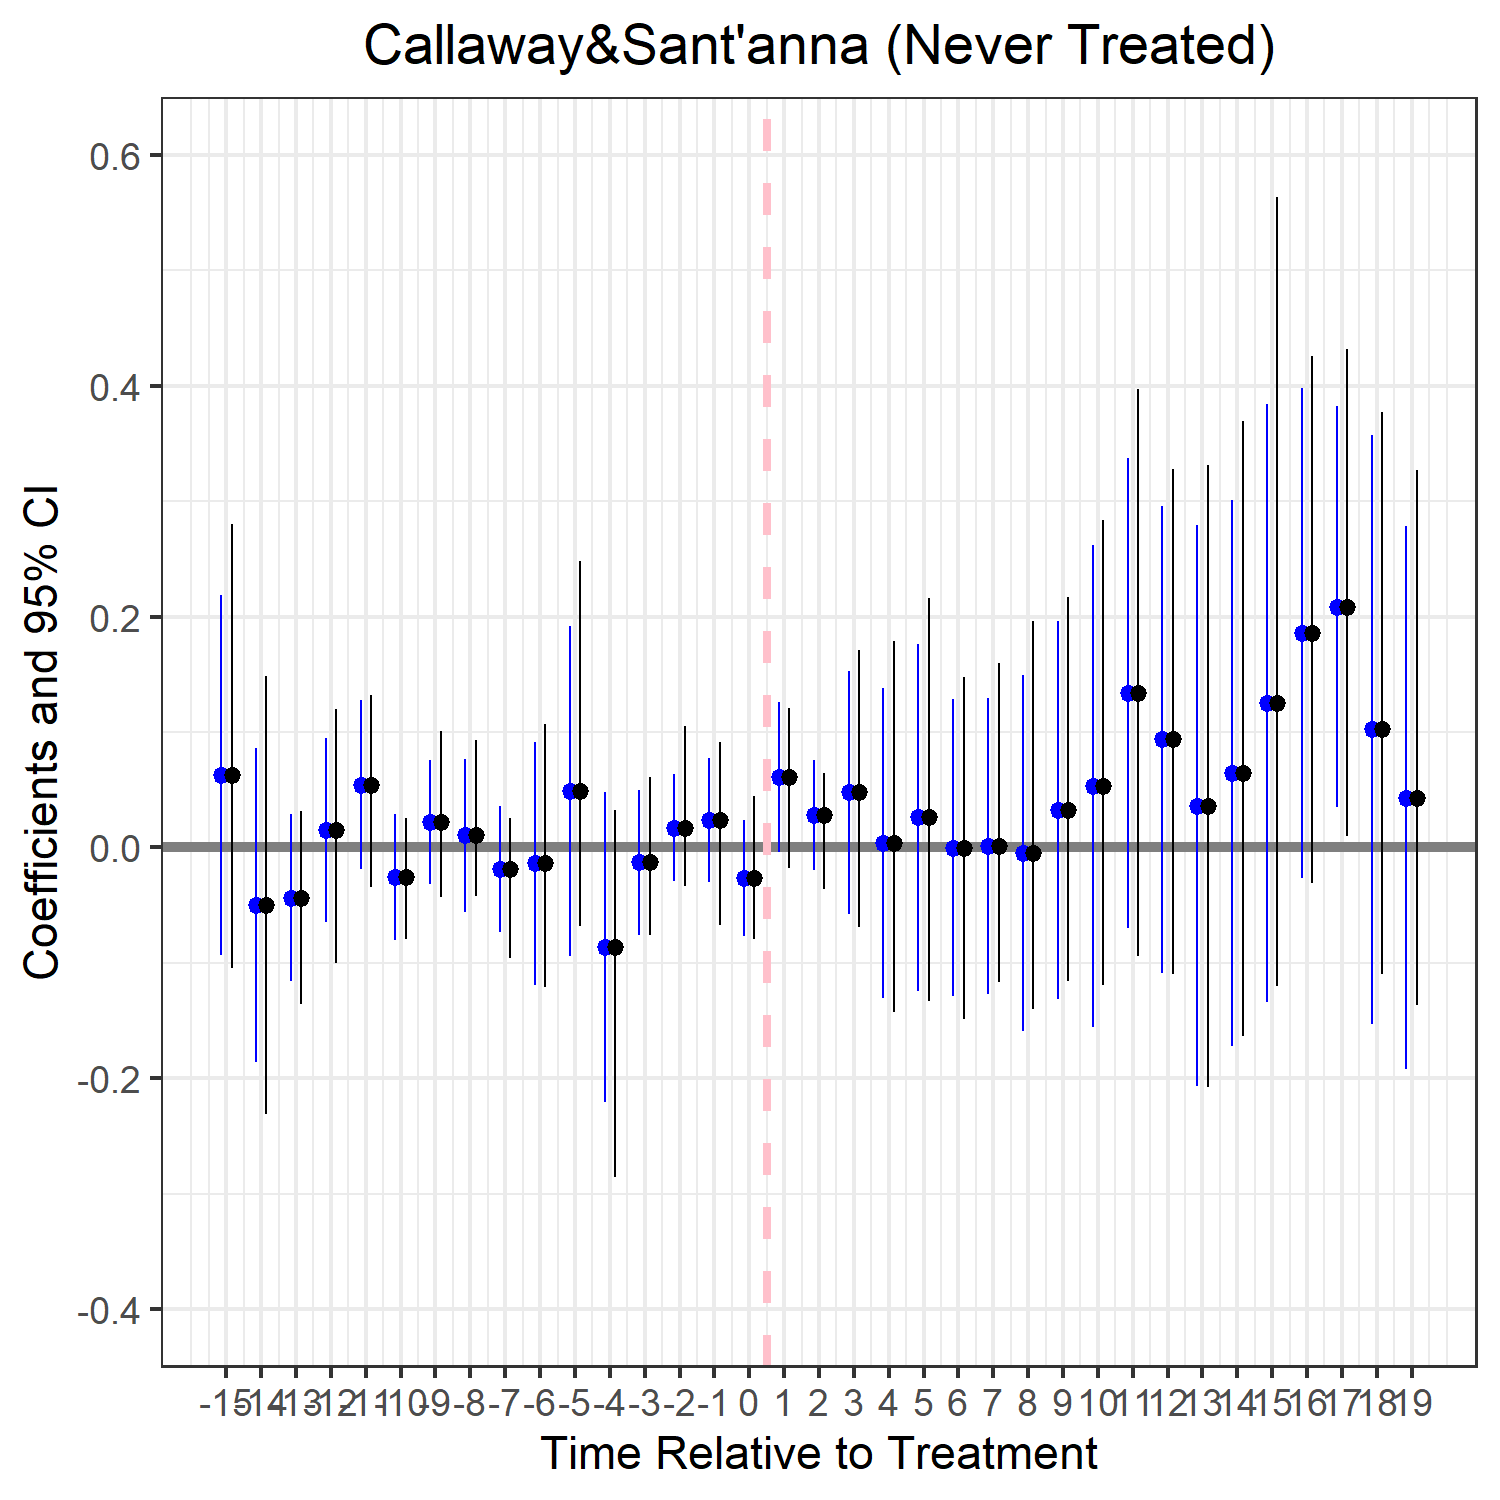
\includegraphics[width=\linewidth, height=0.27\textheight, keepaspectratio]{bischof_cs2.png}
\par{\scriptsize CSDID (never-treated)}}
\end{column}
\begin{column}{0.32\textwidth}
\centering
\onslide<4->{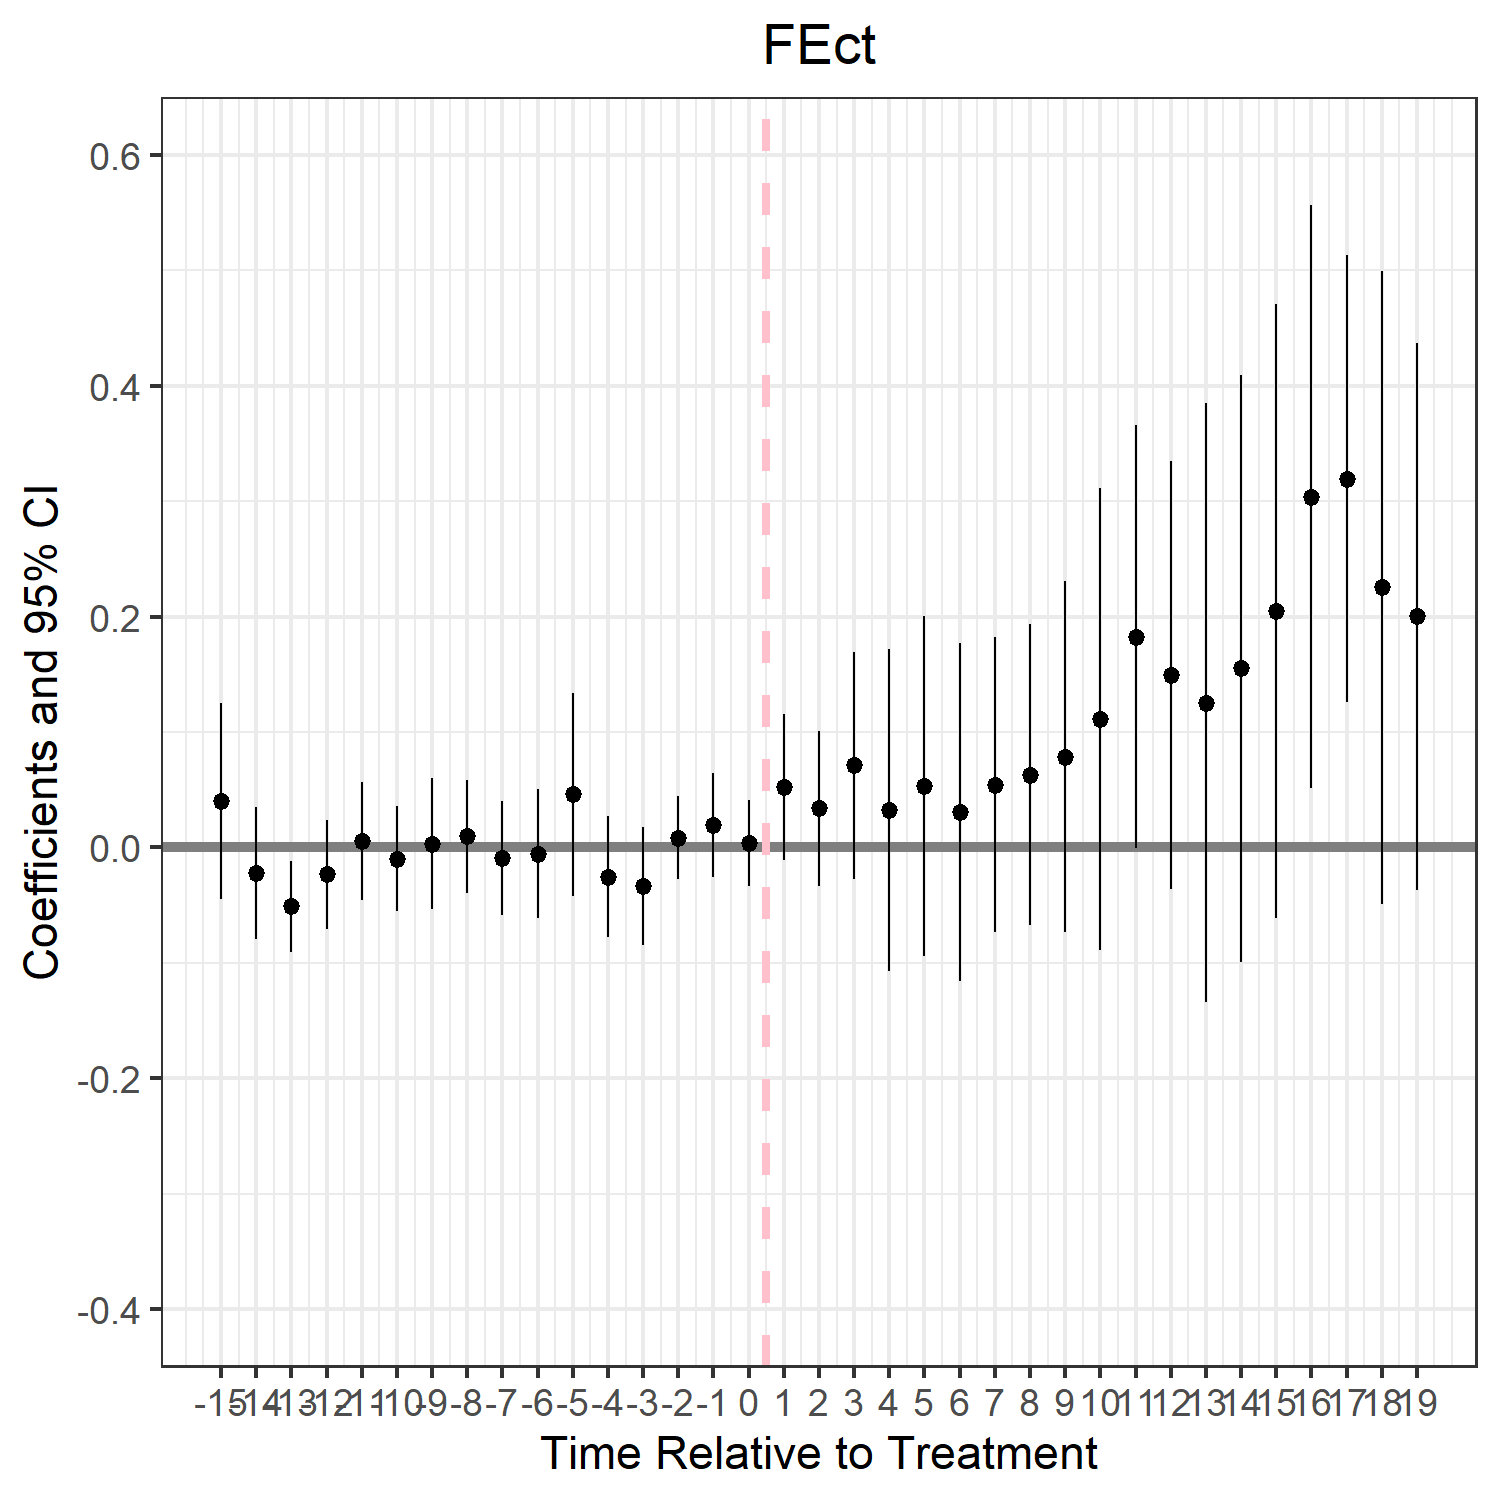
\includegraphics[width=\linewidth, height=0.27\textheight, keepaspectratio]{bischof_fect.png}
\par{\scriptsize imputation (FEct)}}
\end{column}
\end{columns}
\medskip
\begin{itemize}
\item<5-> \textcite{bischof2019voters}: the estimators tell one story; when parallel trends looks plausible, agreement is the norm
\end{itemize}
\end{frame}

\begin{frame}
  \frametitle{Example 1: Coethnic Mobilization (\cite{grumbach2020race})}
\begin{columns}[T,onlytextwidth]
\begin{column}{0.52\textwidth}
\begin{itemize}\itemsep0.6em
\item Do ethnic minority candidates mobilize coethnic donors?
\begin{itemize}\itemsep0.3em
  \item Unit of analysis: 498 US congressional districts, 1980--2012
  \item Treatment: Asian (vs. White, Black, and Hispanic) candidates in general elections
  \item Outcome: percentage of Asian donations
\end{itemize}
\item<2-> The treatment matrix is unbalanced with missing data; the imputation approach handles it without reweighting gymnastics
\end{itemize}
\end{column}
\begin{column}{0.46\textwidth}
\centering
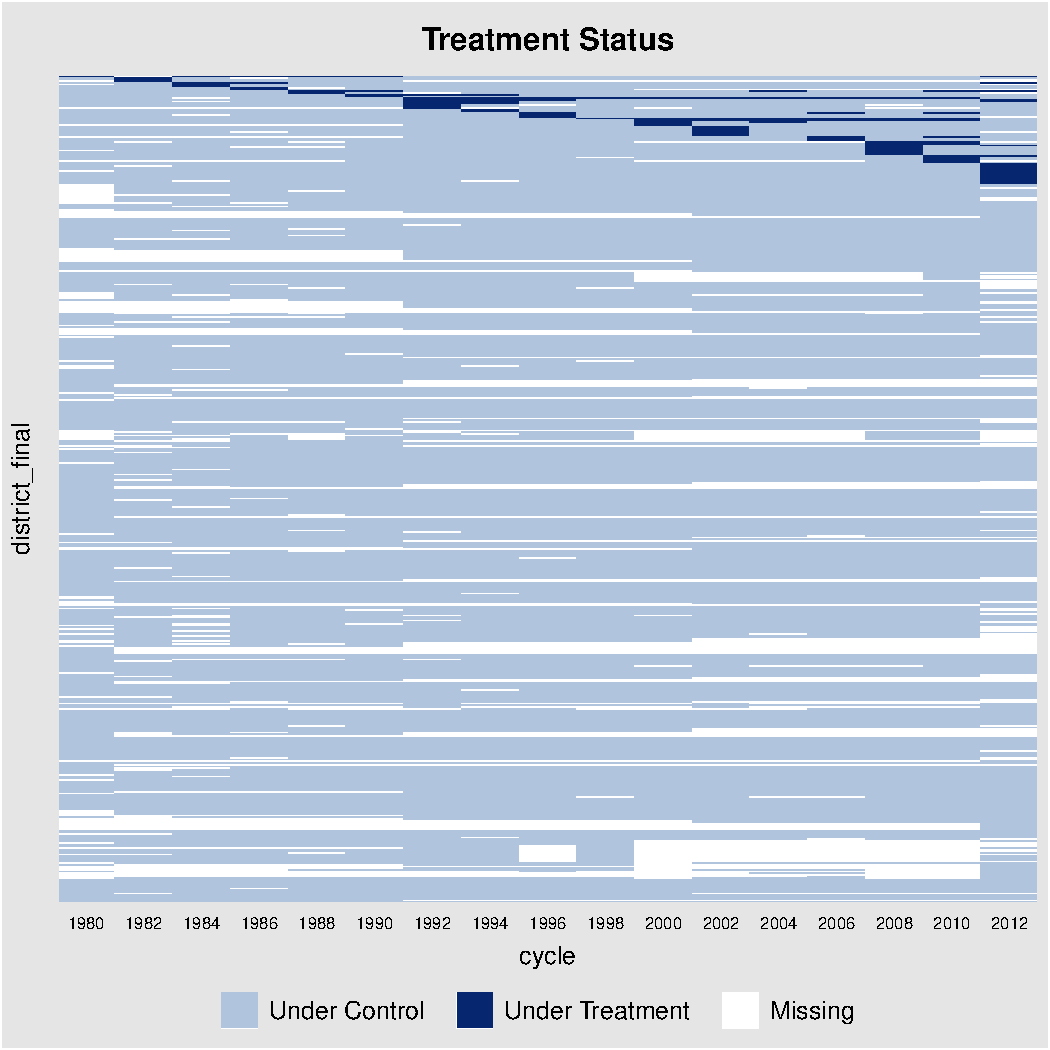
\includegraphics[width=\linewidth, height=0.74\textheight, keepaspectratio]{gs2020_treat.pdf}
\end{column}
\end{columns}
\end{frame}

\begin{frame}
  \frametitle{Effects Are Heterogeneous}
\begin{columns}[T,onlytextwidth]
\begin{column}{0.46\textwidth}
\medskip
\begin{itemize}[<+->]\itemsep1em
\item Effects grow over calendar time: exactly the heterogeneity that breaks the single-$\tau$ TWFE regression
\item Do the HTE-robust estimators change the answer here?
\end{itemize}
\end{column}
\begin{column}{0.52\textwidth}
\centering
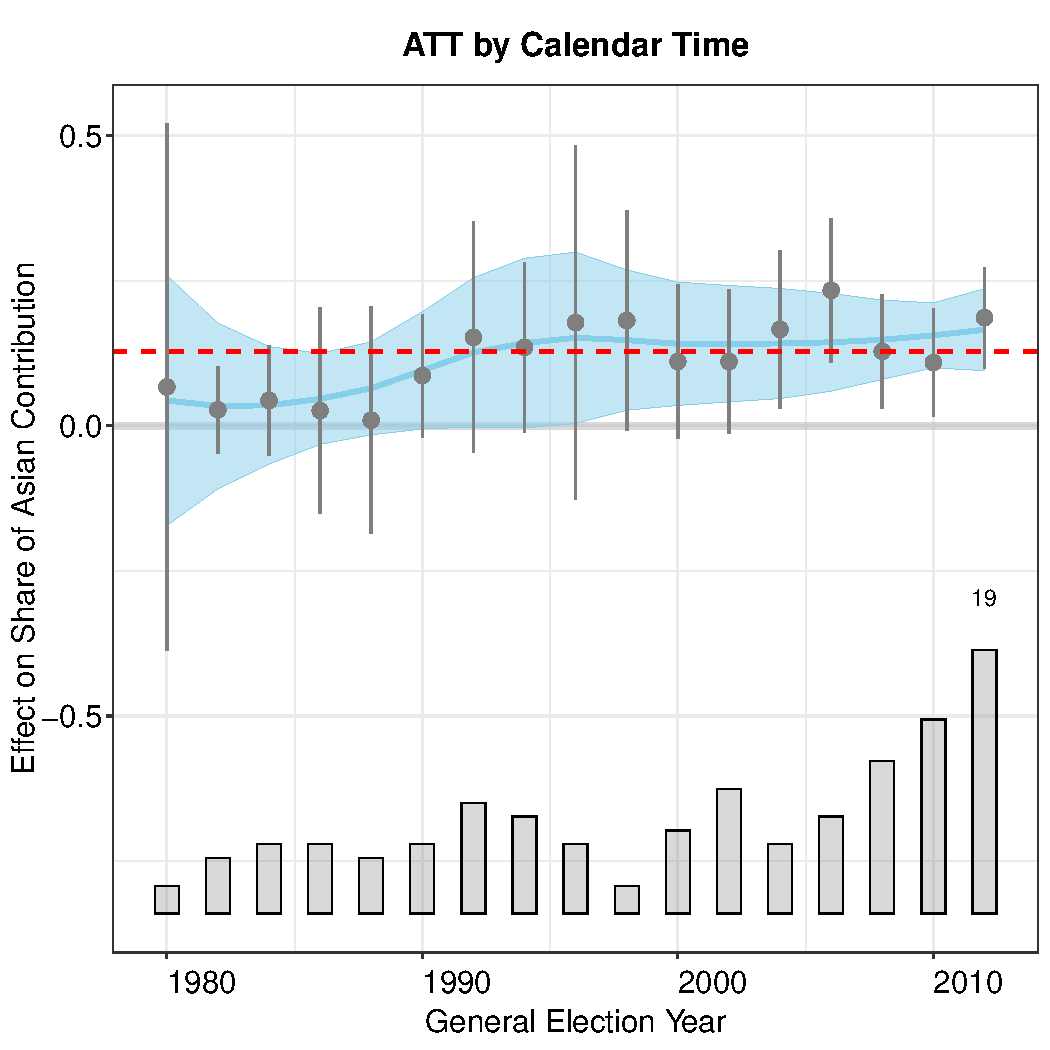
\includegraphics[width=\linewidth, height=0.74\textheight, keepaspectratio]{gs2020_hte_time.pdf}
\end{column}
\end{columns}
\end{frame}

\begin{frame}
  \frametitle{Do the Estimators Agree in Practice?}
\begin{center}
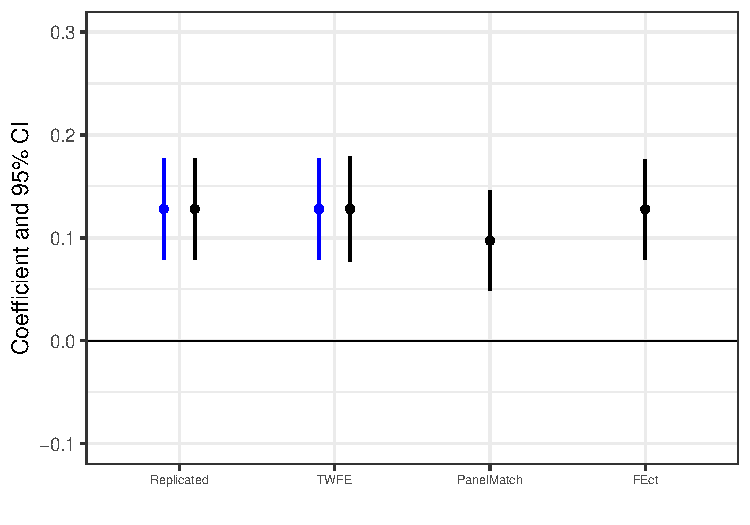
\includegraphics[width=0.8\textwidth, height=0.58\textheight, keepaspectratio]{grumbach_compare.pdf}
\end{center}
\begin{itemize}
\item<2-> \textcite{grumbach2020race}: TWFE, PanelMatch, and FEct give similar answers; here the design is strong and HTE is second-order
\end{itemize}
\end{frame}

\section{Diagnostics and Lessons from 49 Reanalyses}

\begin{frame}
  \frametitle{A Diagnostic Suite Built on Imputation}
The imputation approach turns identification checks into estimable quantities:
\bigskip
\begin{itemize}[<+->]\itemsep1em
\item \textbf{Pre-trend $F$ test}: are the average $\hat{\delta}_{it}$ in pre-treatment periods jointly zero?
\item \textbf{Placebo test}: hide the last few pre-treatment periods from estimation, then check the ``effect'' in the hidden periods
\item \textbf{Carryover test}: hide the first few \alert{post-exit} periods, then check for lingering effects after treatment ends
\item \textbf{Equivalence (TOST) tests}: instead of failing to reject zero, reject pre-trends larger than a tolerance; more informative in well-powered settings
\end{itemize}
\end{frame}

\begin{frame}
  \frametitle{The Suite Applied to Example 1 (\cite{grumbach2020race})}
\begin{columns}[T,onlytextwidth]
\begin{column}{0.32\textwidth}
\centering
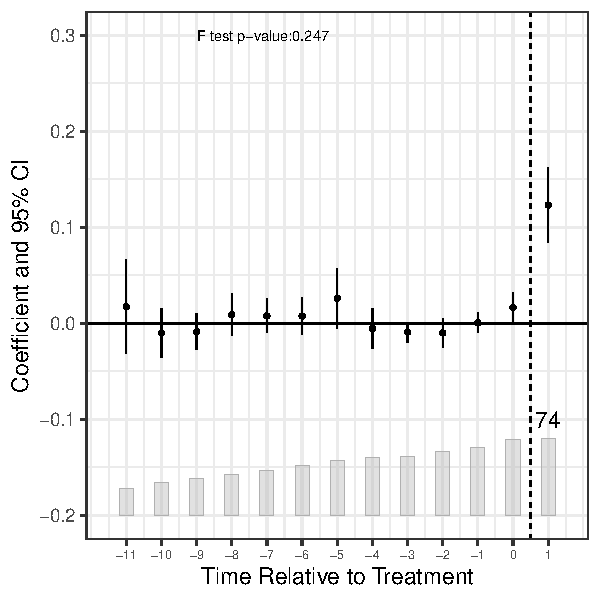
\includegraphics[width=\linewidth]{gs2020_fect.pdf}
\par{\scriptsize $F$ test for no pre-trend}
\end{column}
\begin{column}{0.32\textwidth}
\centering
\onslide<2->{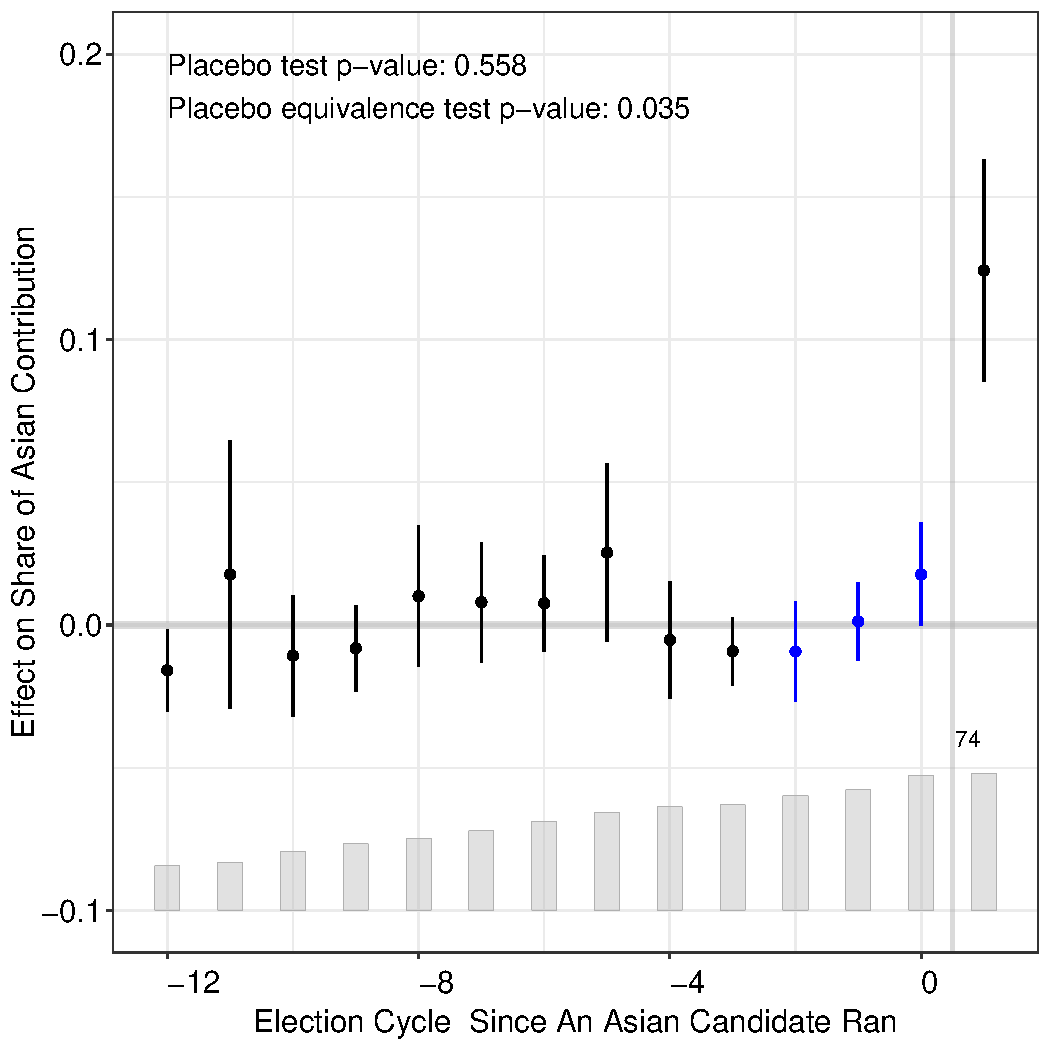
\includegraphics[width=\linewidth]{gs2020_placebo.pdf}
\par{\scriptsize placebo test}}
\end{column}
\begin{column}{0.32\textwidth}
\centering
\onslide<3->{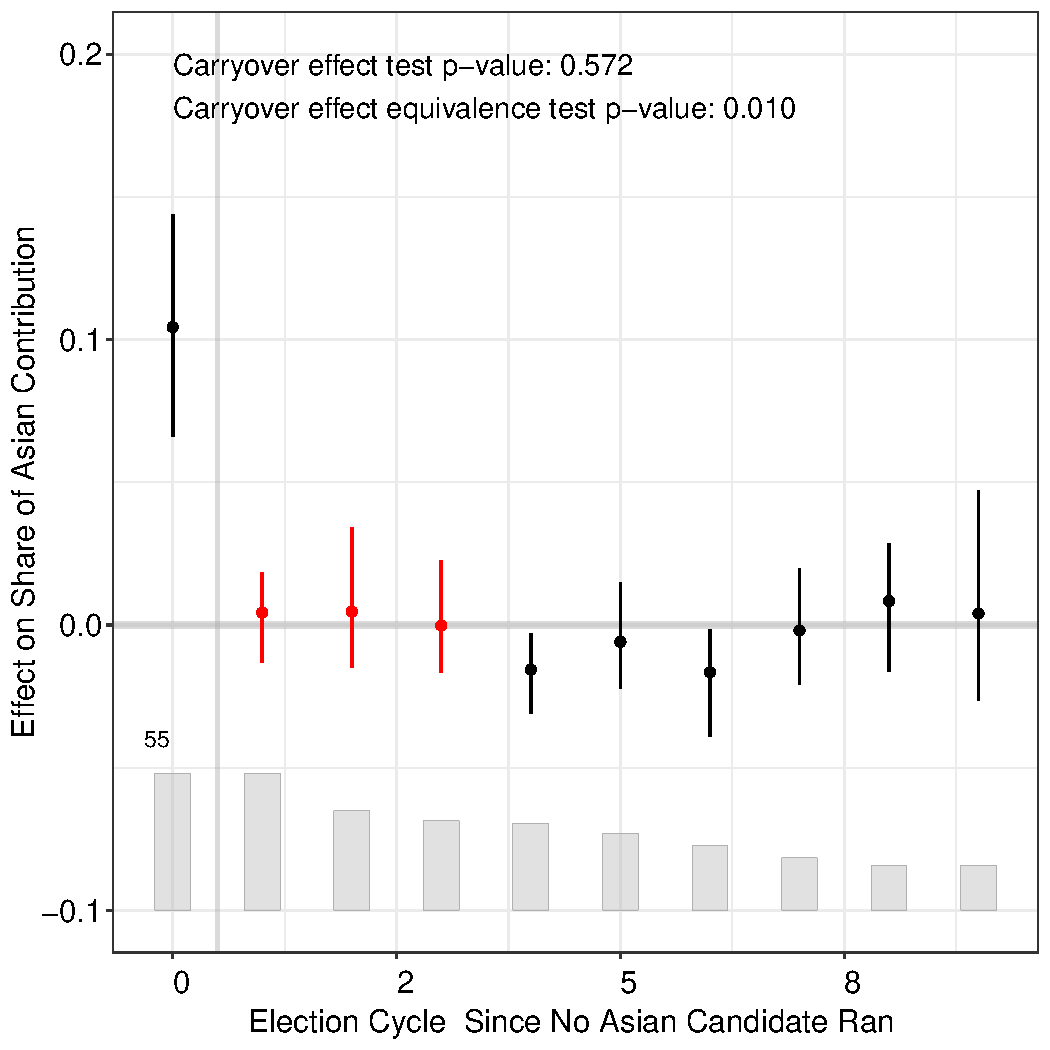
\includegraphics[width=\linewidth]{gs2020_carryover.pdf}
\par{\scriptsize carryover test}}
\end{column}
\end{columns}
\bigskip
\begin{itemize}
\item<4-> None of the three rejects its null here; with 74 treated observations, power is the caveat to keep in mind
\end{itemize}
\end{frame}

\begin{frame}[t]
  \frametitle{Example 2: Lawsuits against Land-Use Restrictions (APSR 2020)}
\begin{itemize}\itemsep0.4em
\item Treatment: a Fair Housing Act lawsuit against a city's land-use restrictions; outcome: the share of the city's residents who are non-Hispanic white (California cities, 1970--2010, staggered)
\item<2-> The imputation event-study plot slopes downward \alert{before} treatment: the pre-trend $F$ test and the placebo test both reject ($p < 0.001$)
\end{itemize}
\medskip
\begin{columns}[T,onlytextwidth]
\begin{column}{0.49\textwidth}\centering
{\footnotesize dynamic effects, with the pre-trend $F$ test}\par\smallskip
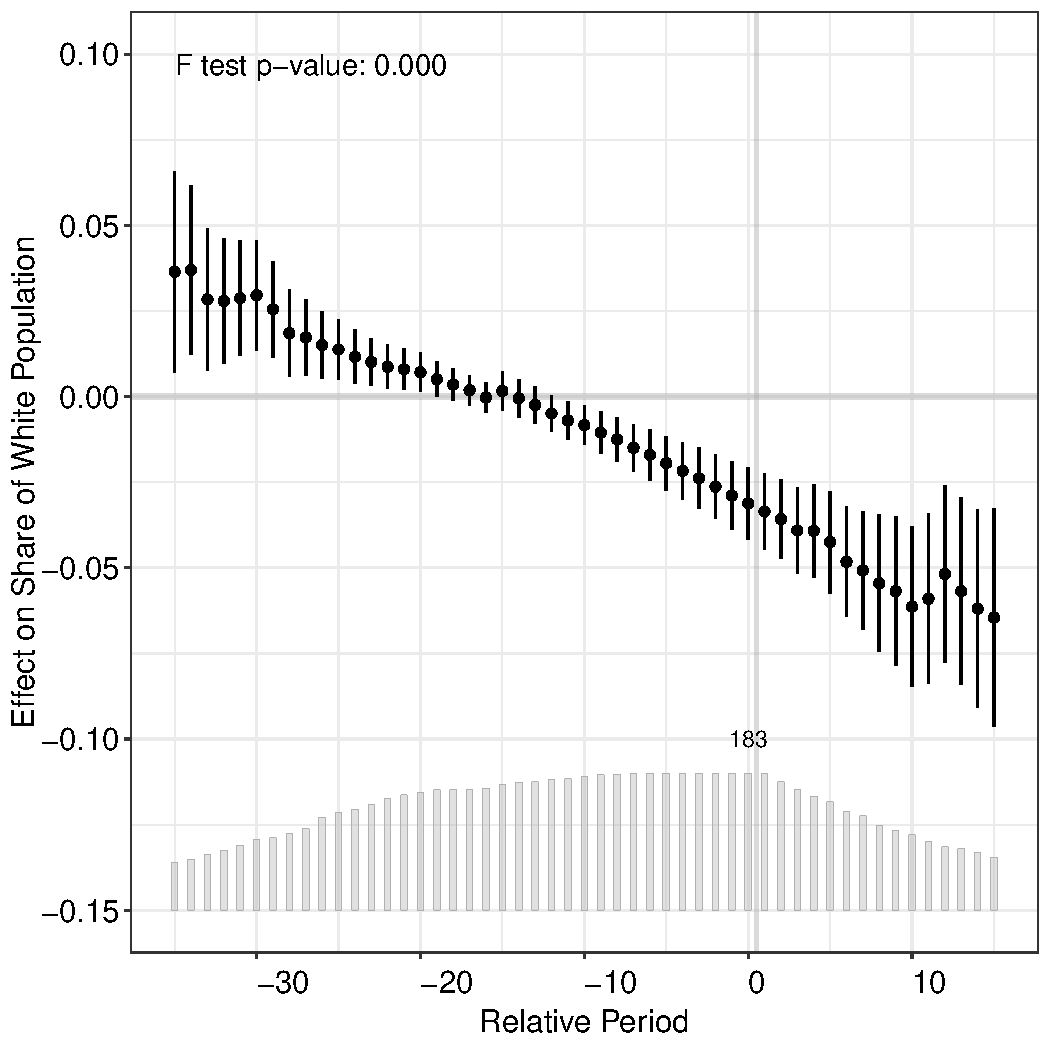
\includegraphics[width=\linewidth, height=0.52\textheight, keepaspectratio]{ex2_gap_long.pdf}
\end{column}
\begin{column}{0.49\textwidth}\centering
\onslide<2->{{\footnotesize placebo test (blue: the hidden periods)}\par\smallskip
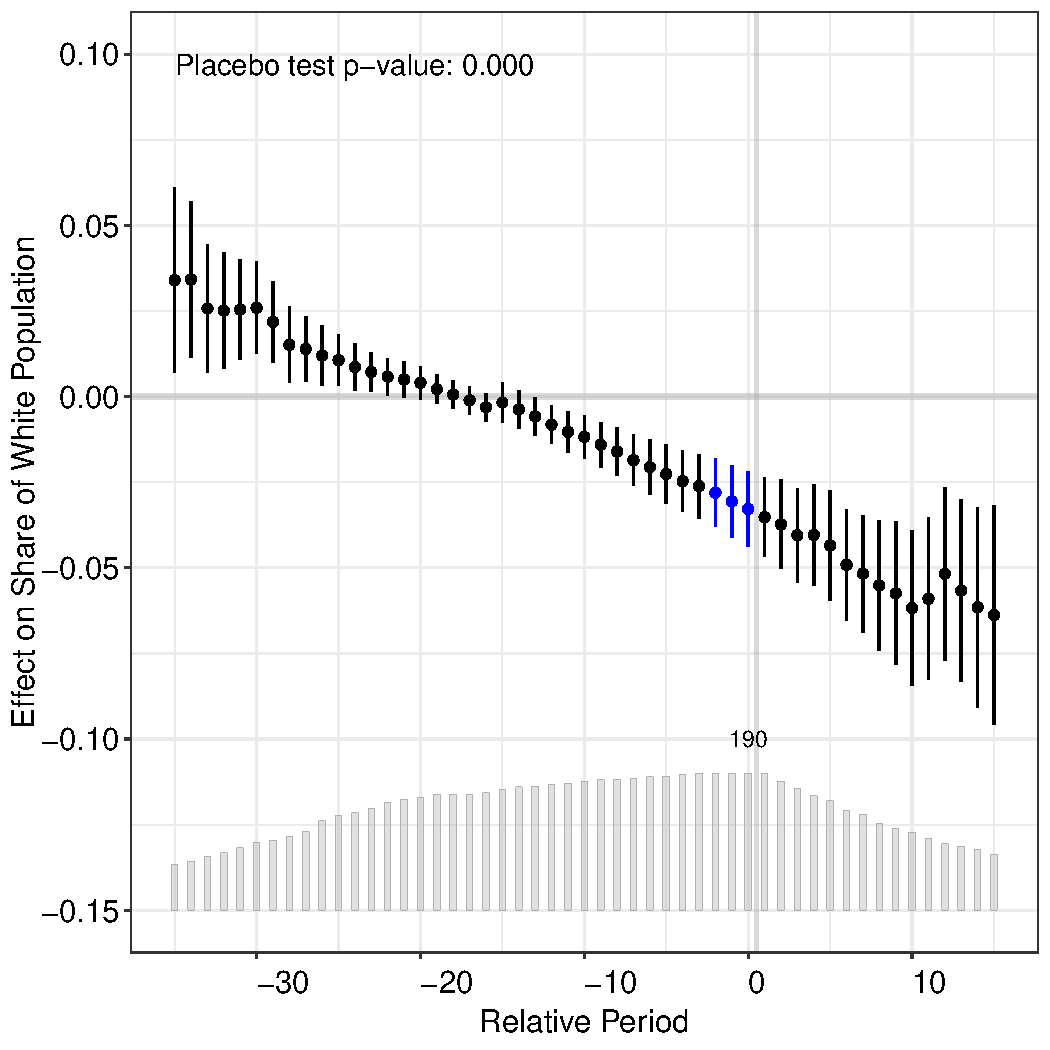
\includegraphics[width=\linewidth, height=0.52\textheight, keepaspectratio]{ex2_placebo_long.pdf}}
\end{column}
\end{columns}
\end{frame}

\begin{frame}[t]
  \frametitle{Example 2: Adding City-Specific Linear Time Trends}
\begin{itemize}\itemsep0.4em
\item The demographic series are mostly interpolated between Census years; dropping the interpolated years changes little
\item<2-> Adding \alert{city-specific linear time trends} removes the pre-trend ($F$ test $p = 0.21$) and the negative effect with it, on the same $-3$ to $+2$ window
\item<3-> The downward slope predates the lawsuits; once the trends absorb it, nothing is left
\end{itemize}
\medskip
\begin{columns}[T,onlytextwidth]
\begin{column}{0.49\textwidth}\centering
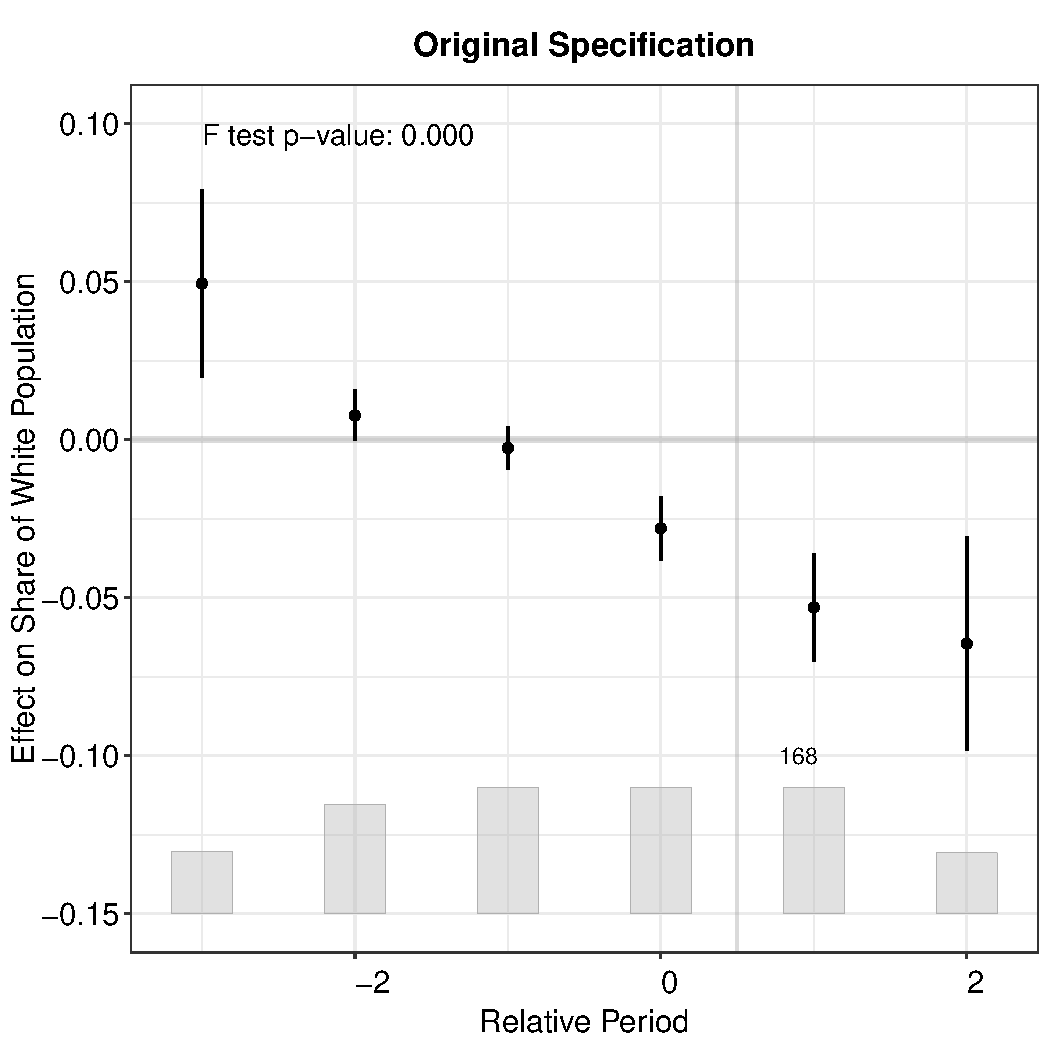
\includegraphics[width=\linewidth, height=0.5\textheight, keepaspectratio]{ex2_gap_short.pdf}
\end{column}
\begin{column}{0.49\textwidth}\centering
\onslide<2->{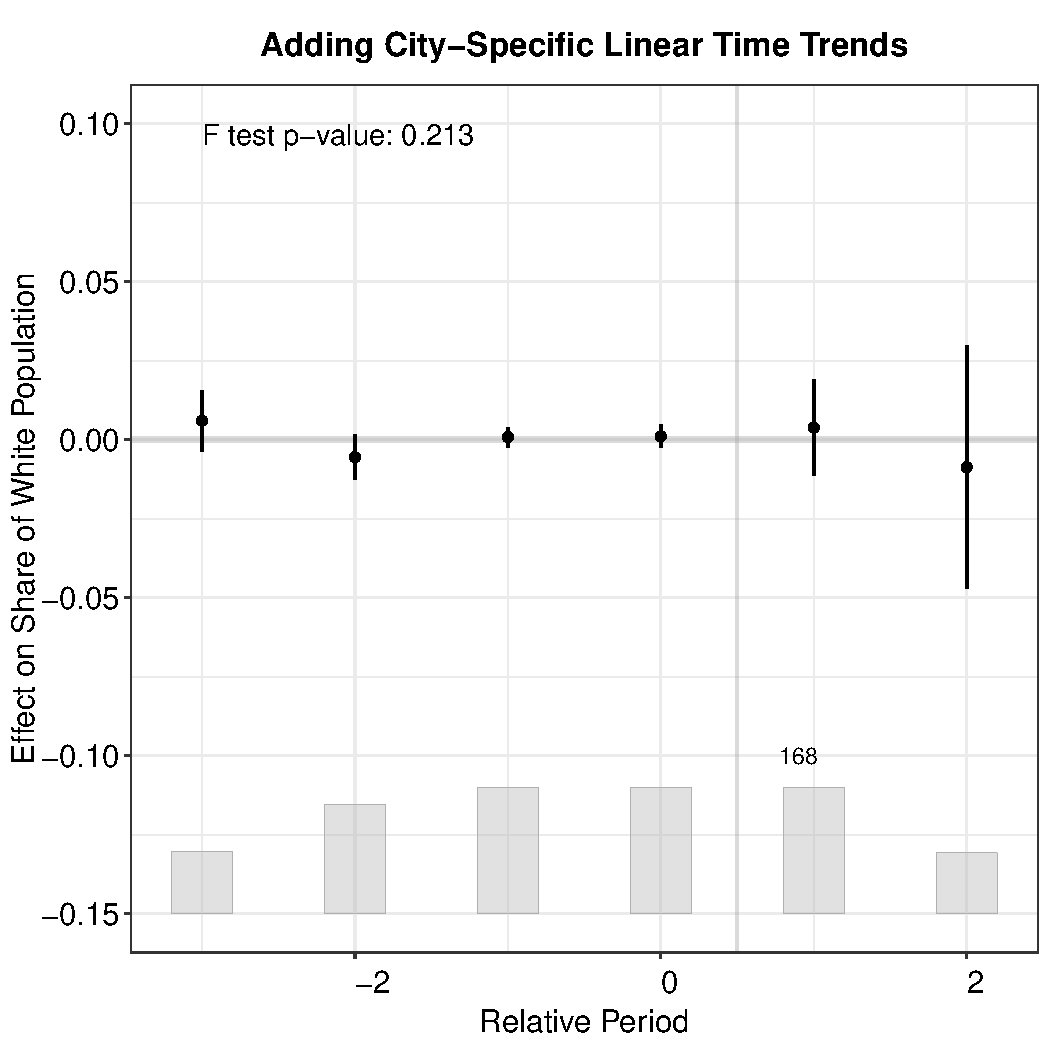
\includegraphics[width=\linewidth, height=0.5\textheight, keepaspectratio]{ex2_lut_gap_short.pdf}}
\end{column}
\end{columns}
\end{frame}

\begin{frame}[t]
  \frametitle{Example 2: The Estimators Still Broadly Agree}
\begin{columns}[T,onlytextwidth]
\begin{column}{0.56\textwidth}
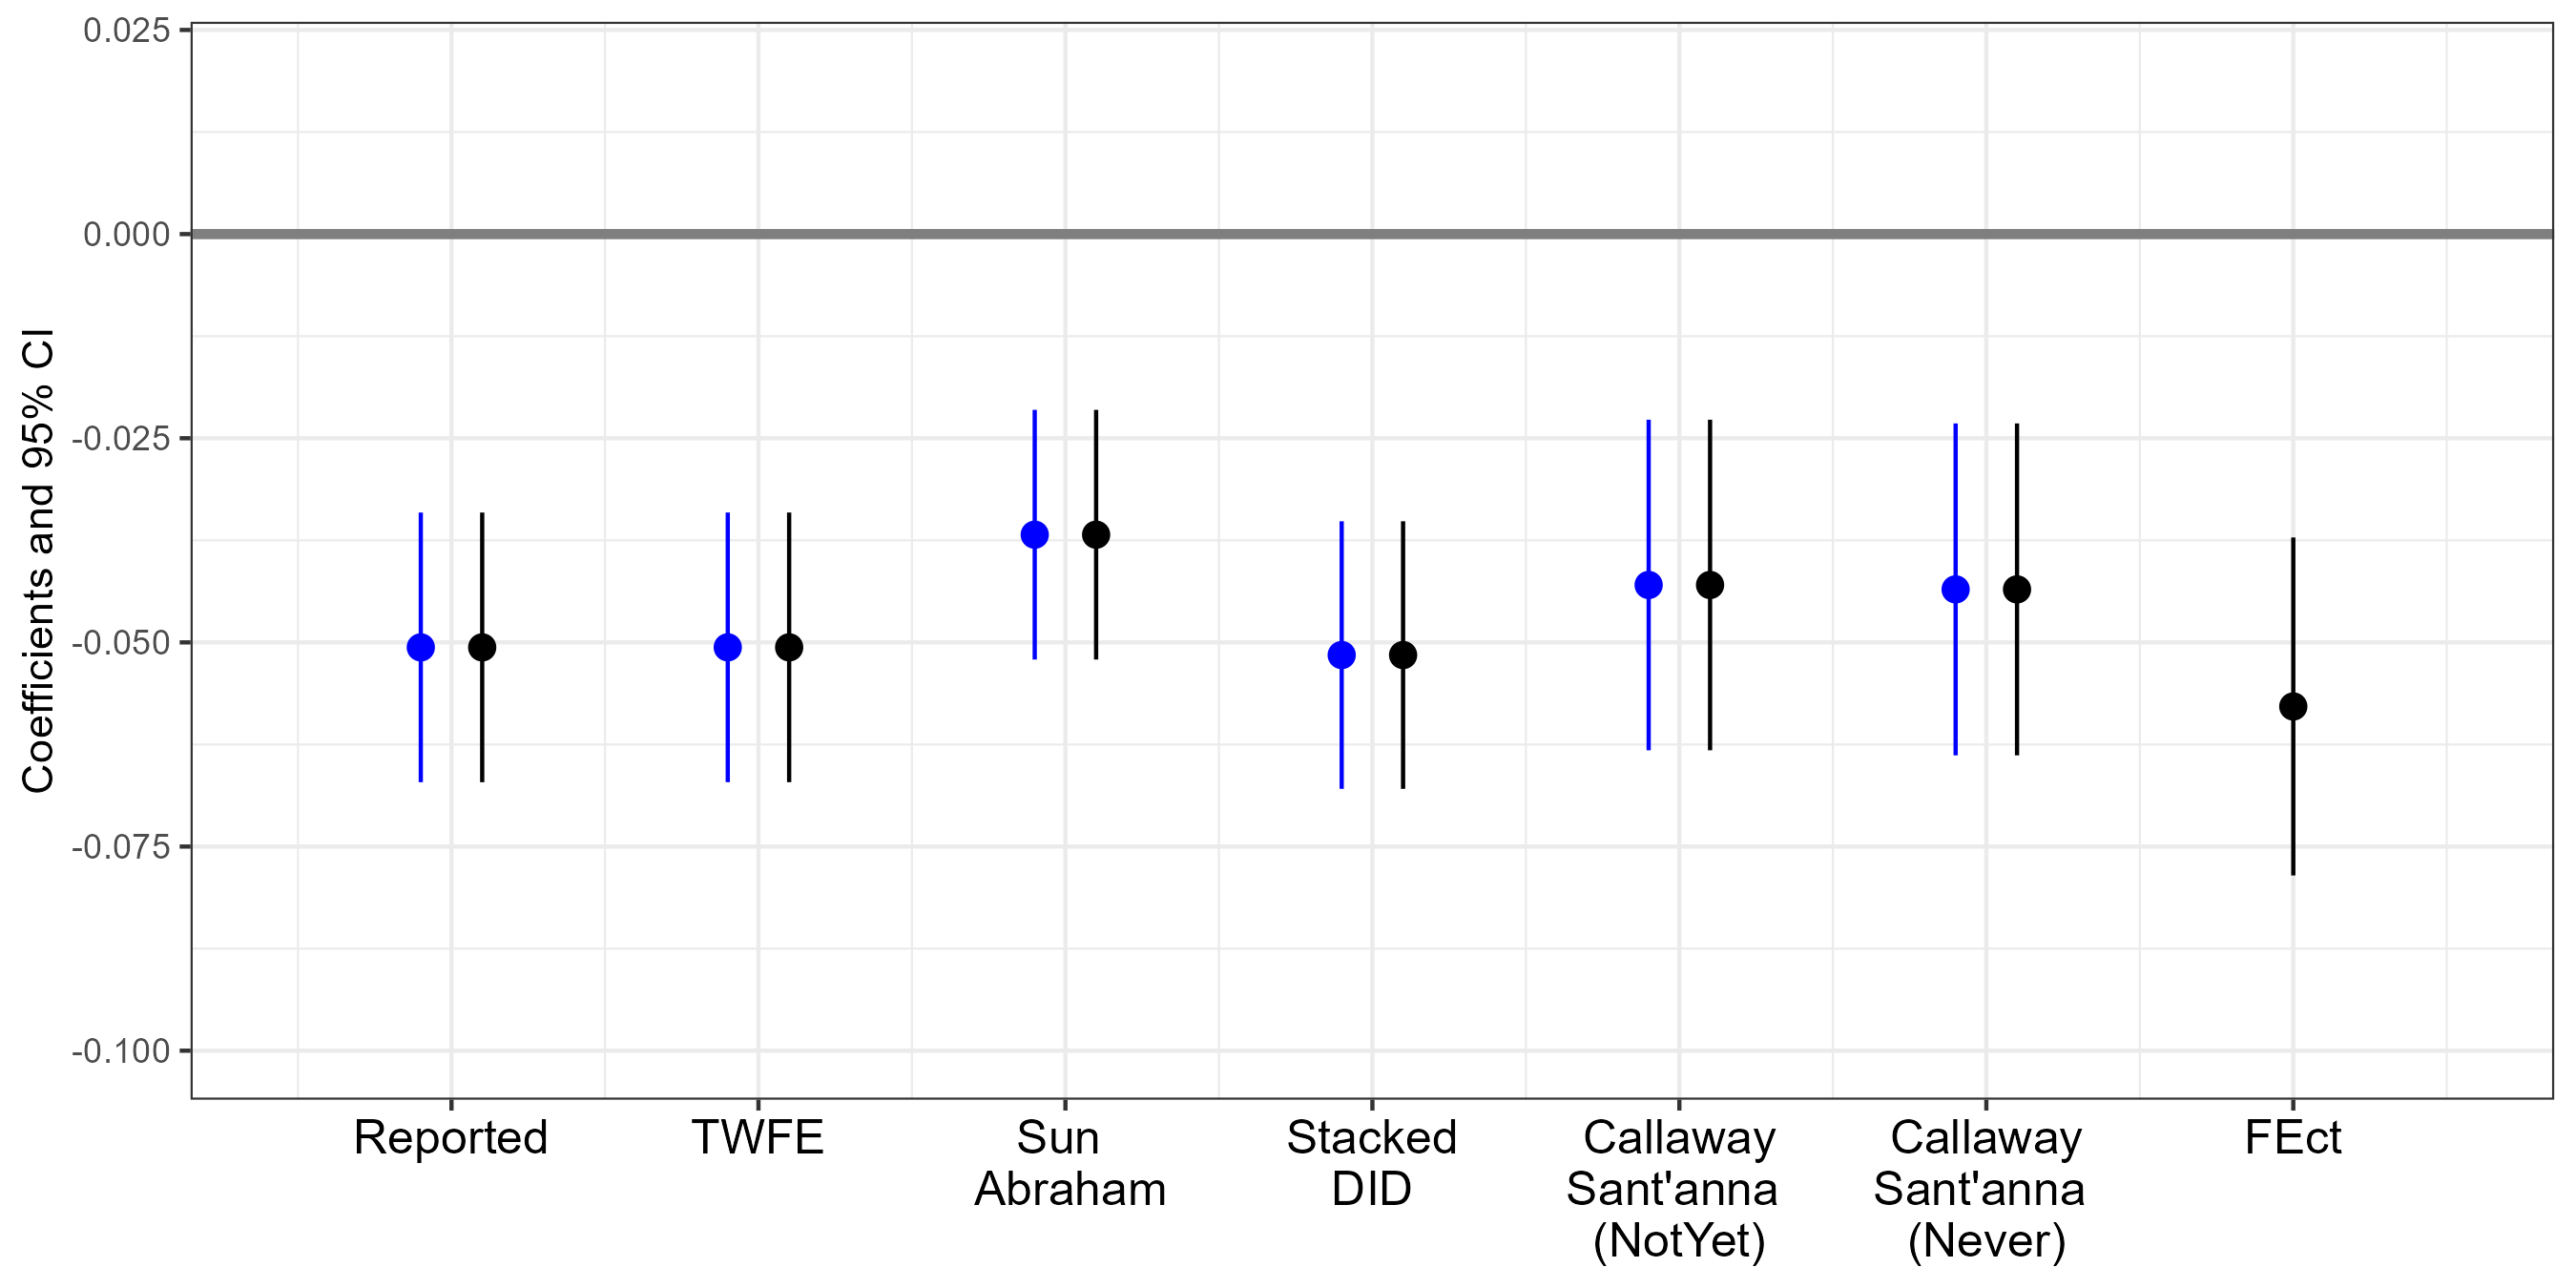
\includegraphics[width=\linewidth]{ex2_estimators.png}
\begin{itemize}\itemsep0.5em
\item<2-> Seven estimators, one answer, about $-0.05$: they all inherit the \alert{same} violated assumption
\item<2-> Agreement across estimators is not robustness; the raw-data plots and the two tests catch what comparing estimators cannot
\end{itemize}
\end{column}
\begin{column}{0.42\textwidth}\centering
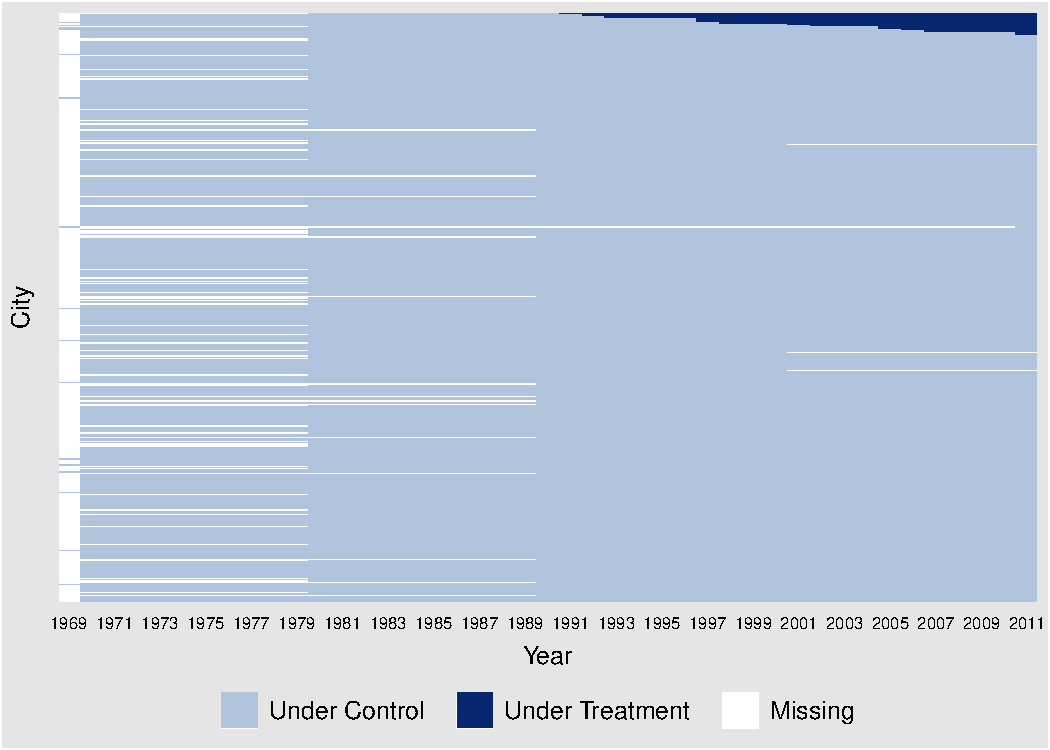
\includegraphics[height=0.28\textheight, keepaspectratio]{ex2_treat.pdf}\par\smallskip
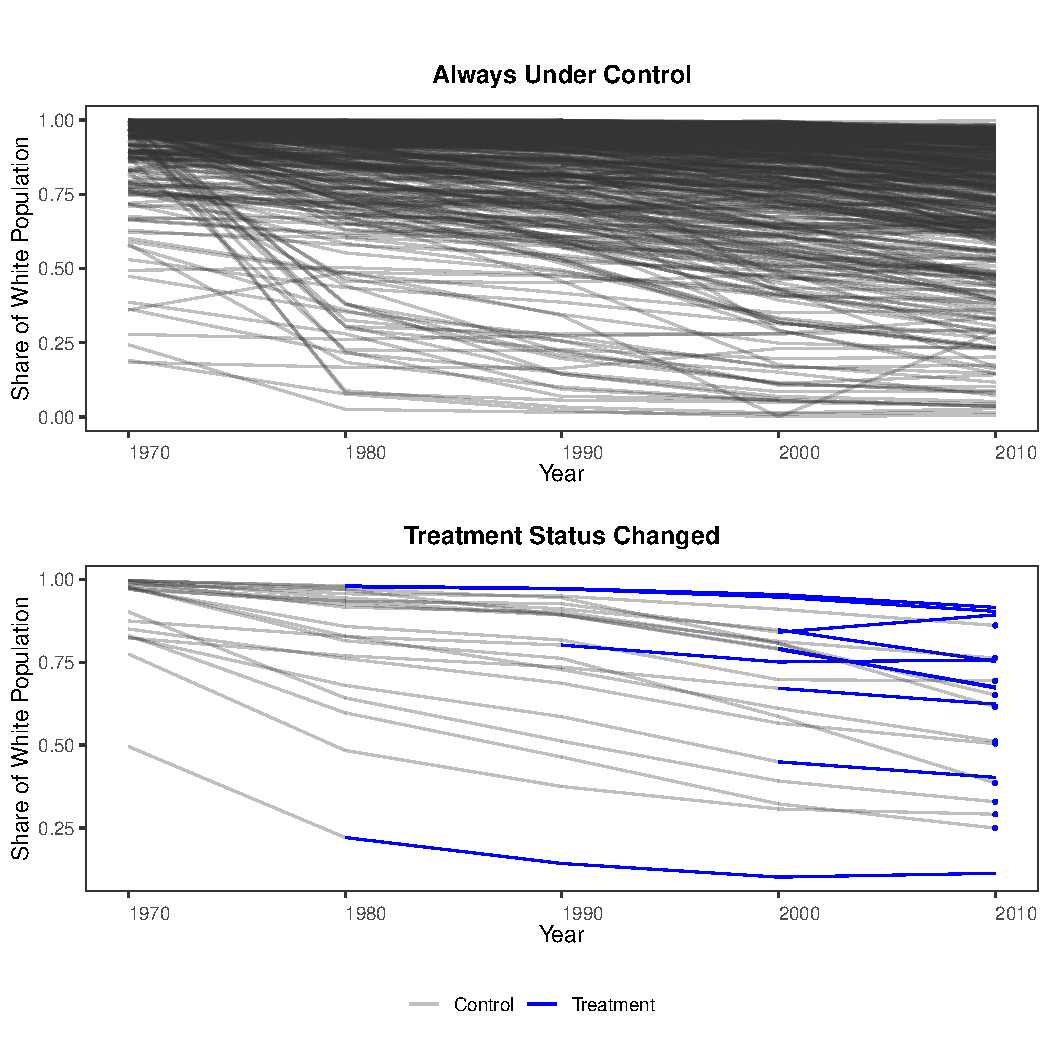
\includegraphics[height=0.44\textheight, keepaspectratio]{ex2_outcome.pdf}
\end{column}
\end{columns}
\end{frame}

\begin{frame}[t]
  \frametitle{Example 3: Updating Cadastral Maps and Property Tax Revenue (JOP 2021)}
\begin{itemize}\itemsep0.4em
\item The authors ask whether updating the cadastral map, the register of properties, raises property tax revenue in Brazilian municipalities (2004--2015, staggered adoption)
\item<2-> Full-sample reanalysis: the estimators \alert{disagree}; the reported estimate is positive, TWFE and CSDID sit near zero, interaction weighting is negative
\item<3-> The paper's event-study specification, replicated on its subsample, shows the positive effect
\end{itemize}
\medskip
\begin{columns}[T,onlytextwidth]
\begin{column}{0.58\textwidth}\centering
\onslide<2->{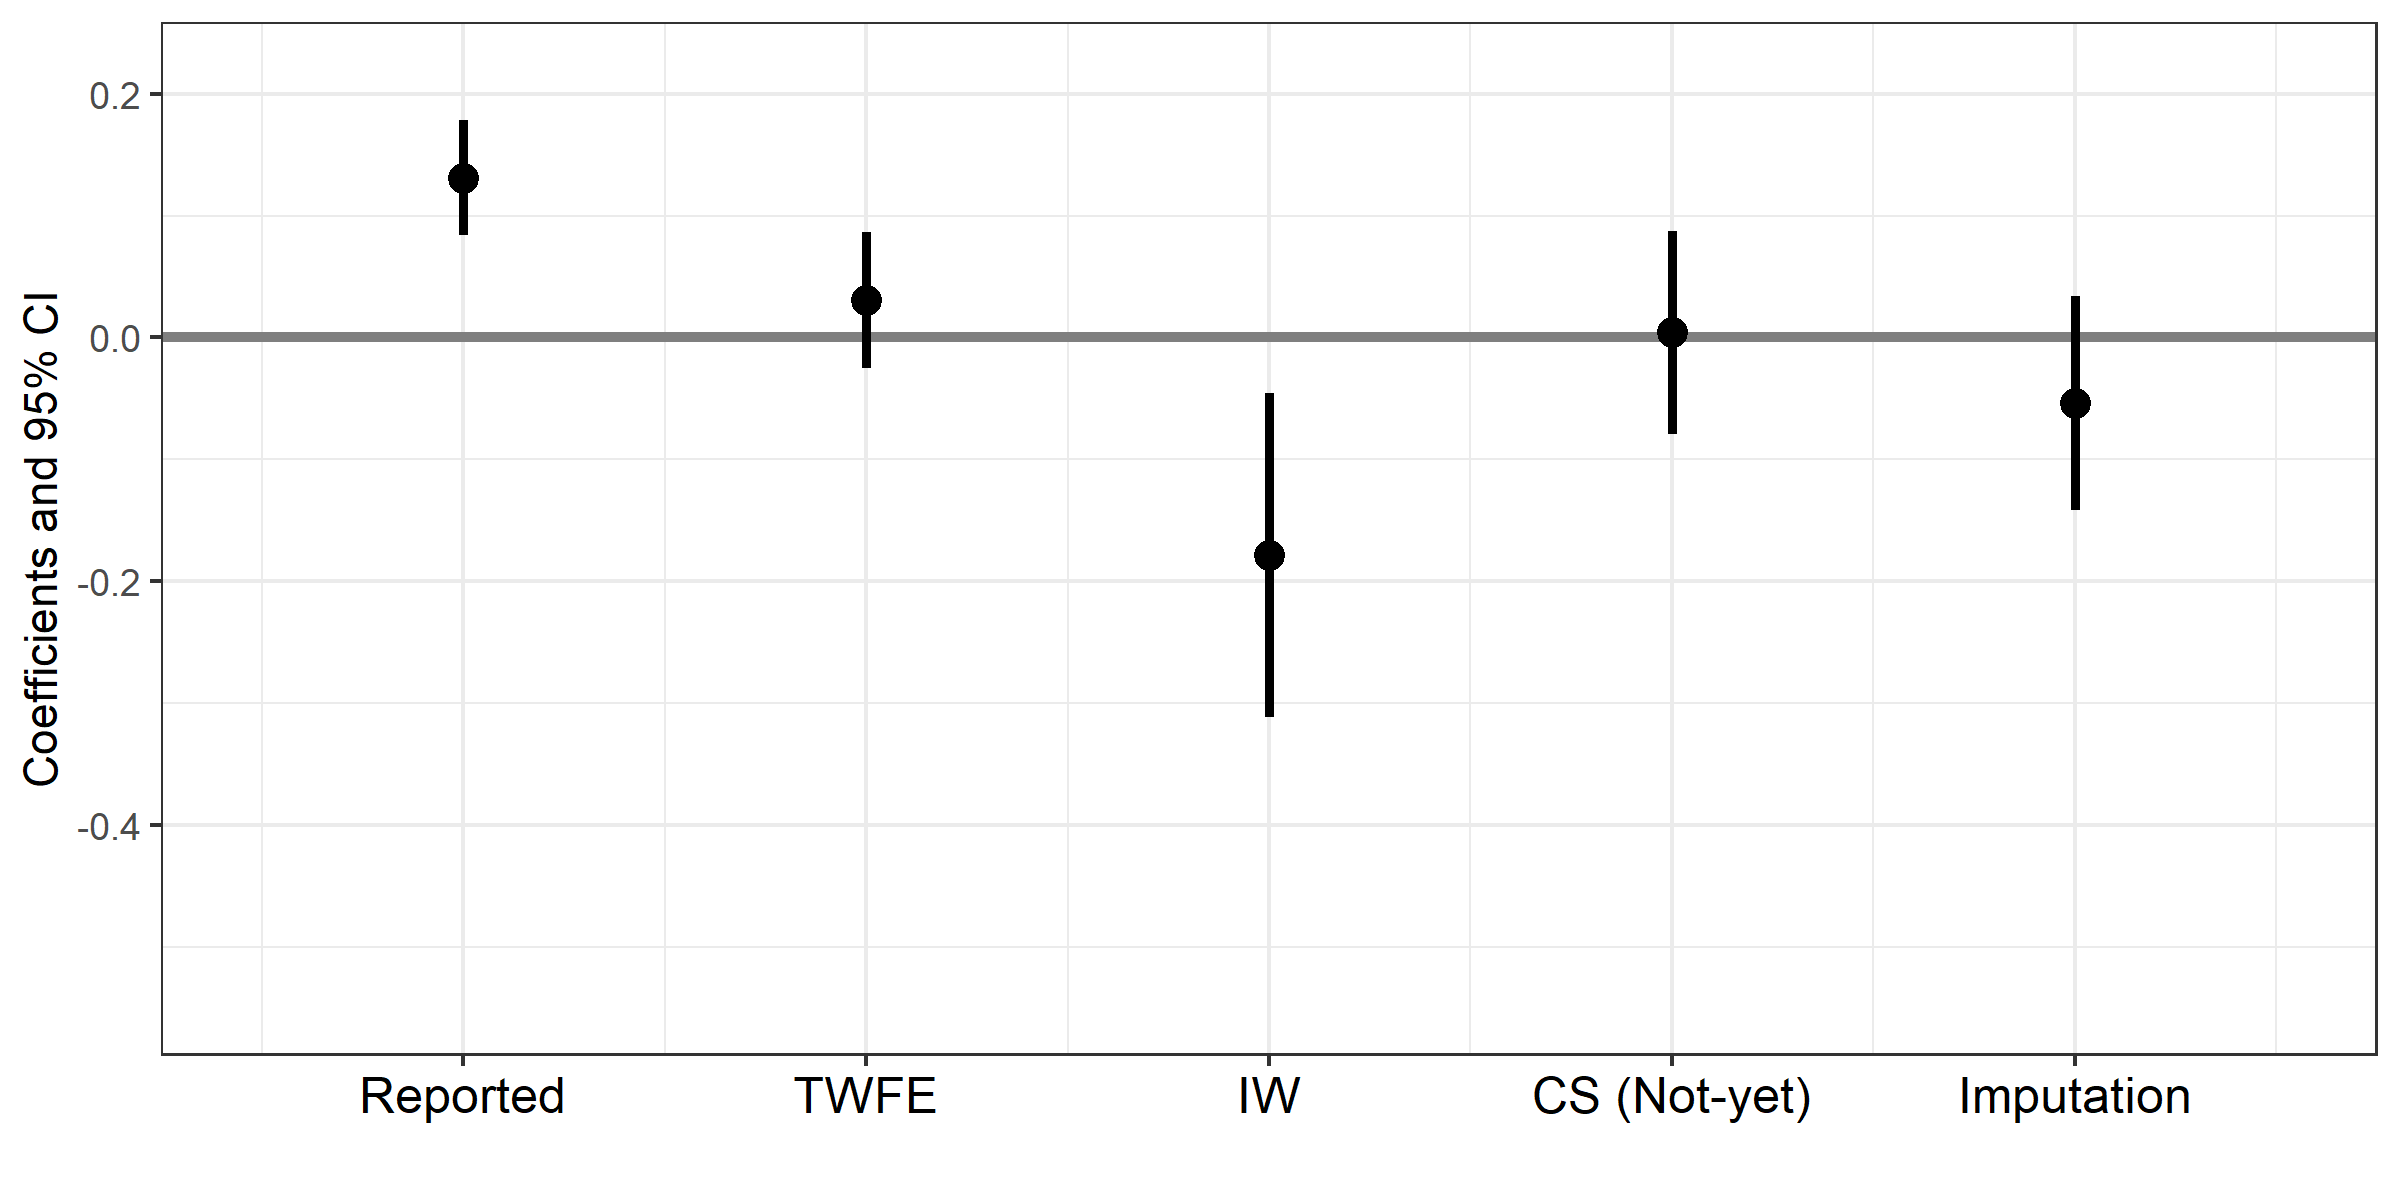
\includegraphics[width=\linewidth, height=0.45\textheight, keepaspectratio]{ex3_compare_full.png}\par{\scriptsize replicated on the full sample}}
\end{column}
\begin{column}{0.4\textwidth}\centering
\onslide<3->{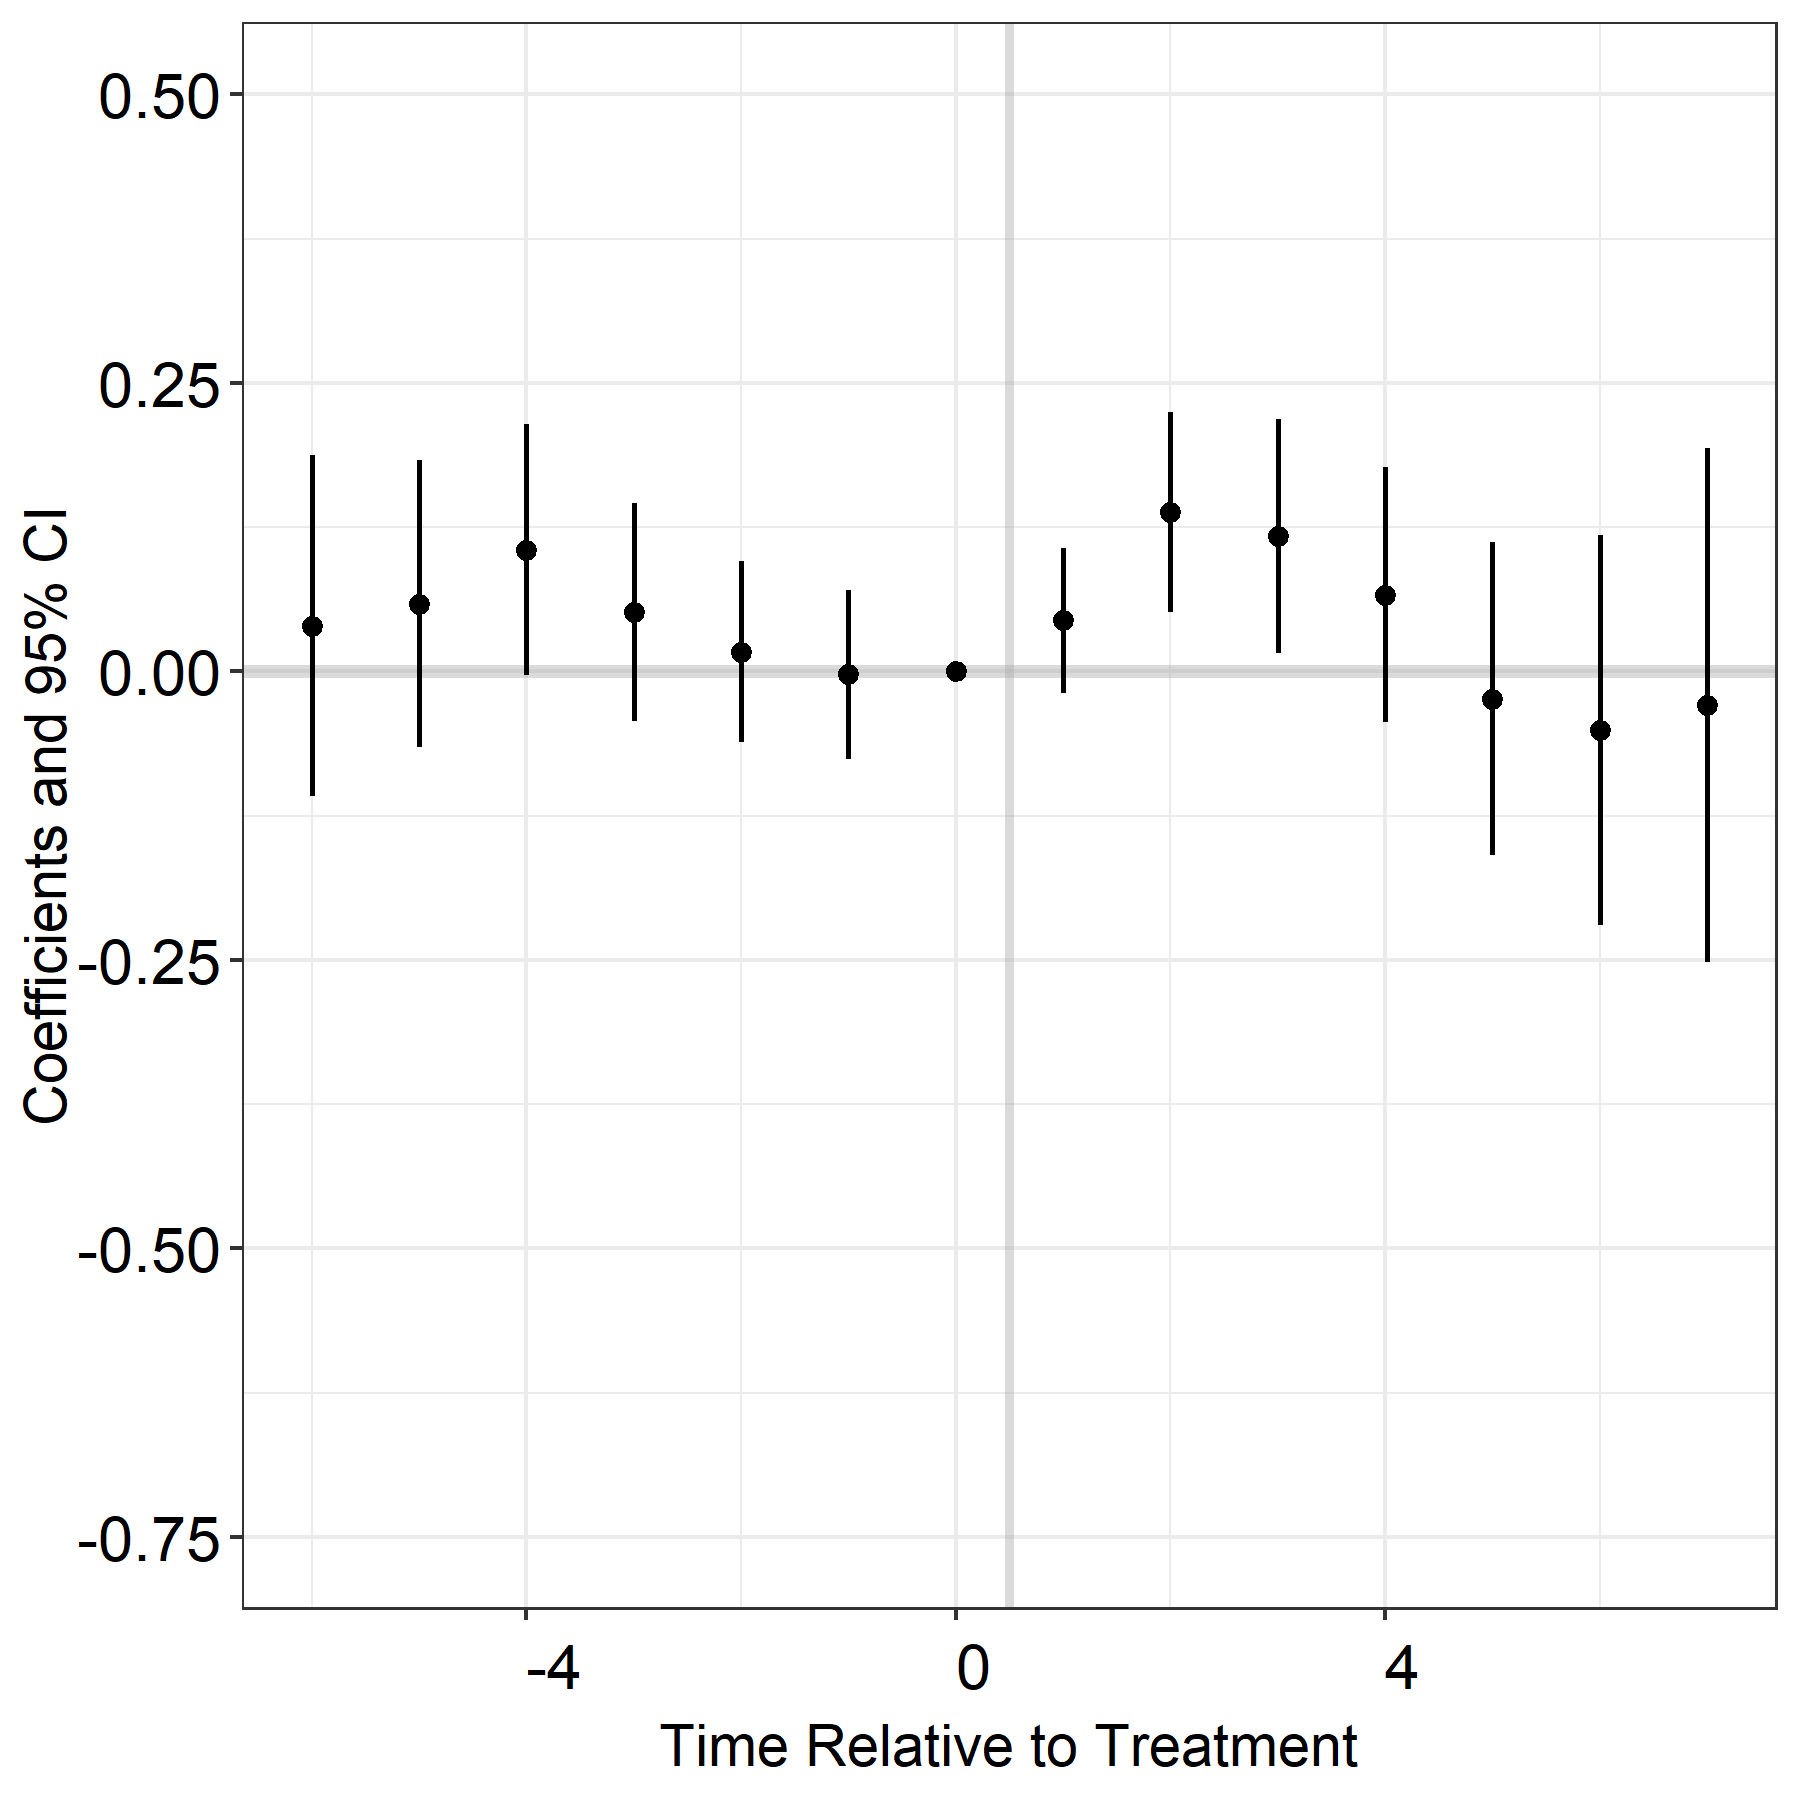
\includegraphics[width=\linewidth, height=0.45\textheight, keepaspectratio]{ex3_sub_twfe.png}\par{\scriptsize the paper's specification on its subsample}}
\end{column}
\end{columns}
\end{frame}

\begin{frame}[t]
  \frametitle{Example 3: Look Deeper}
\begin{columns}[T,onlytextwidth]
\begin{column}{0.36\textwidth}\centering
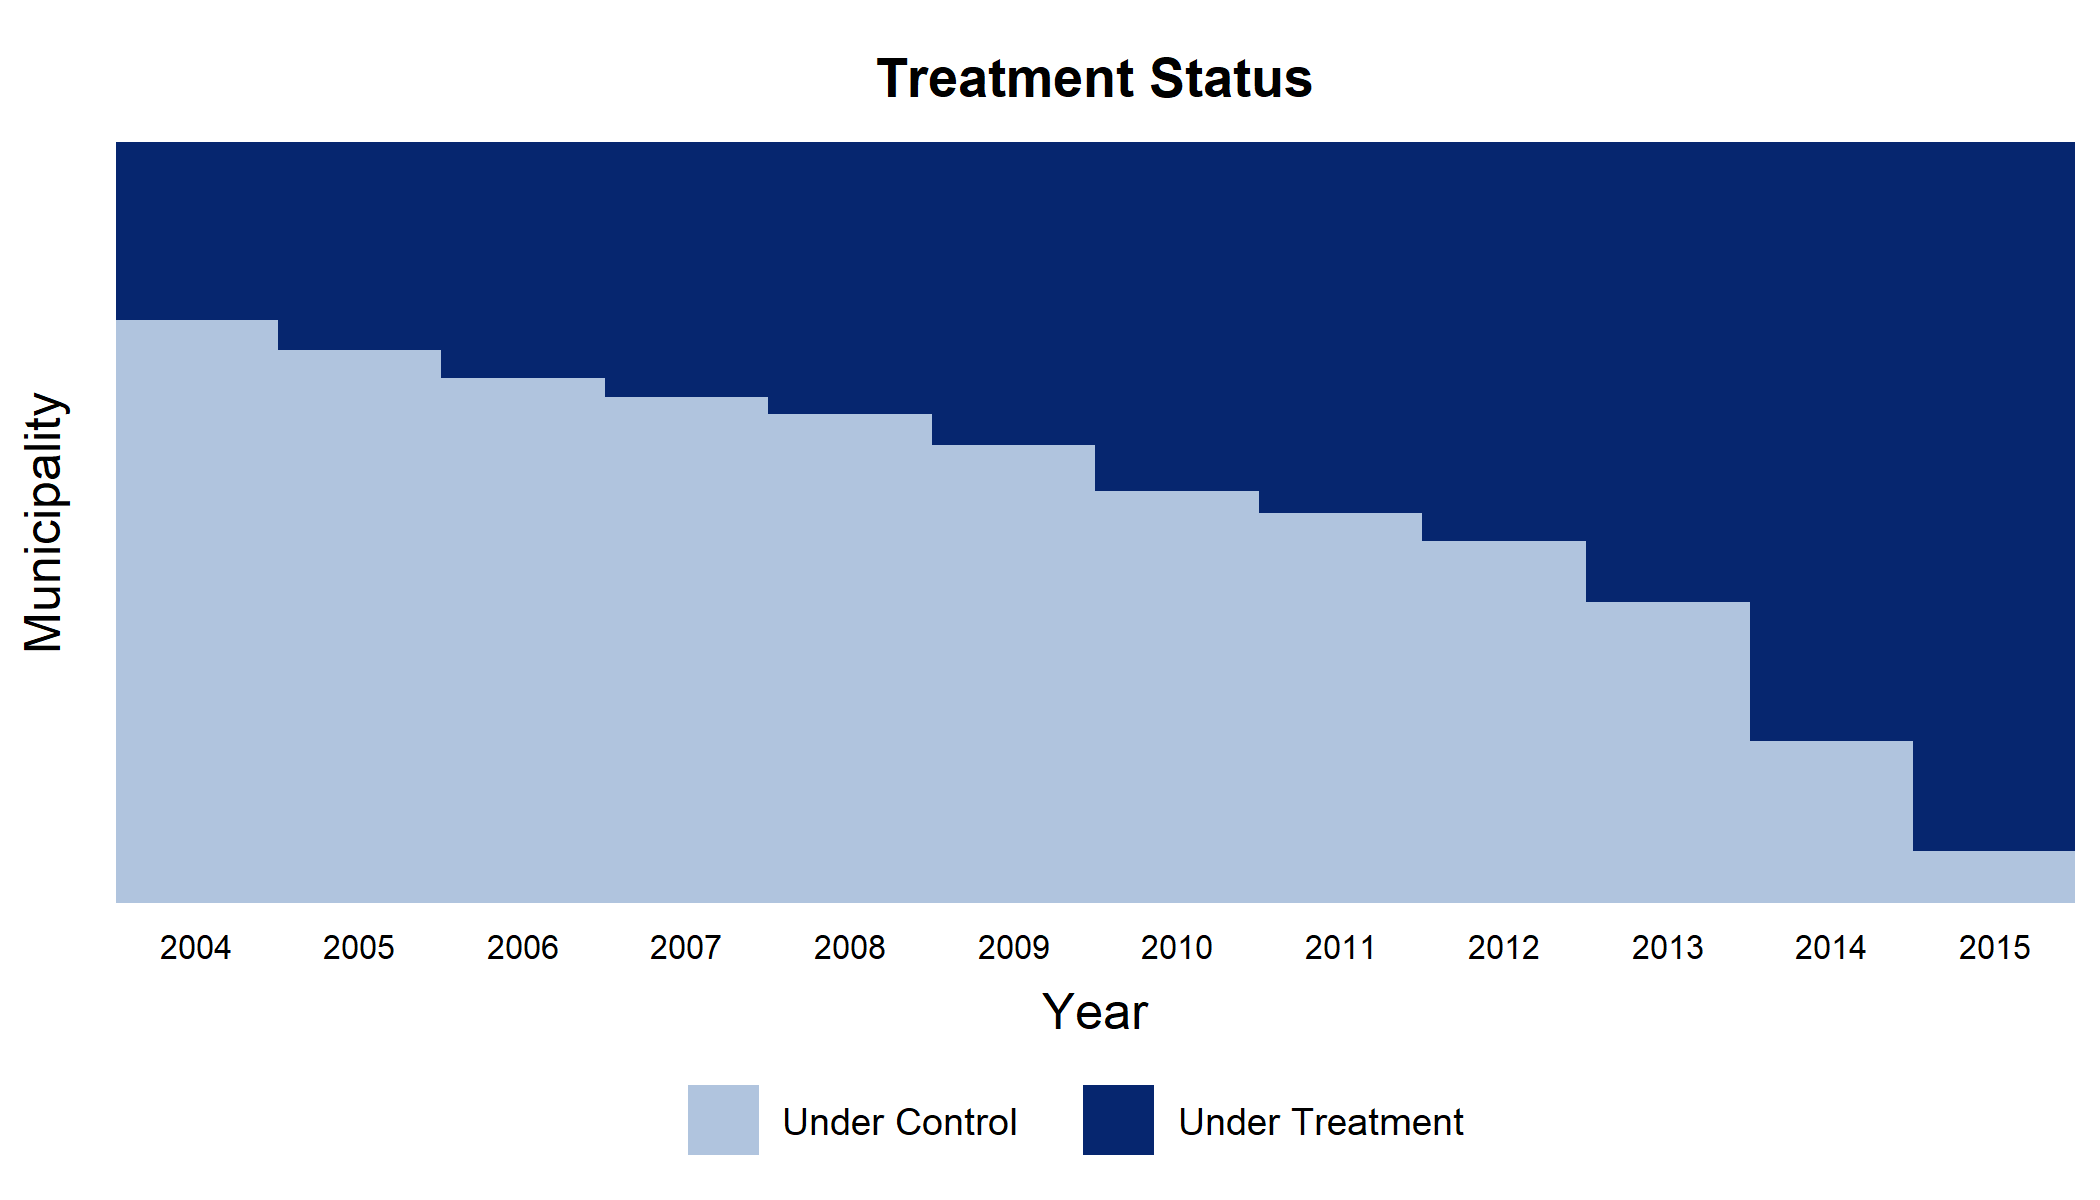
\includegraphics[width=\linewidth]{ex3_treat_pv.png}\par\smallskip
\onslide<2->{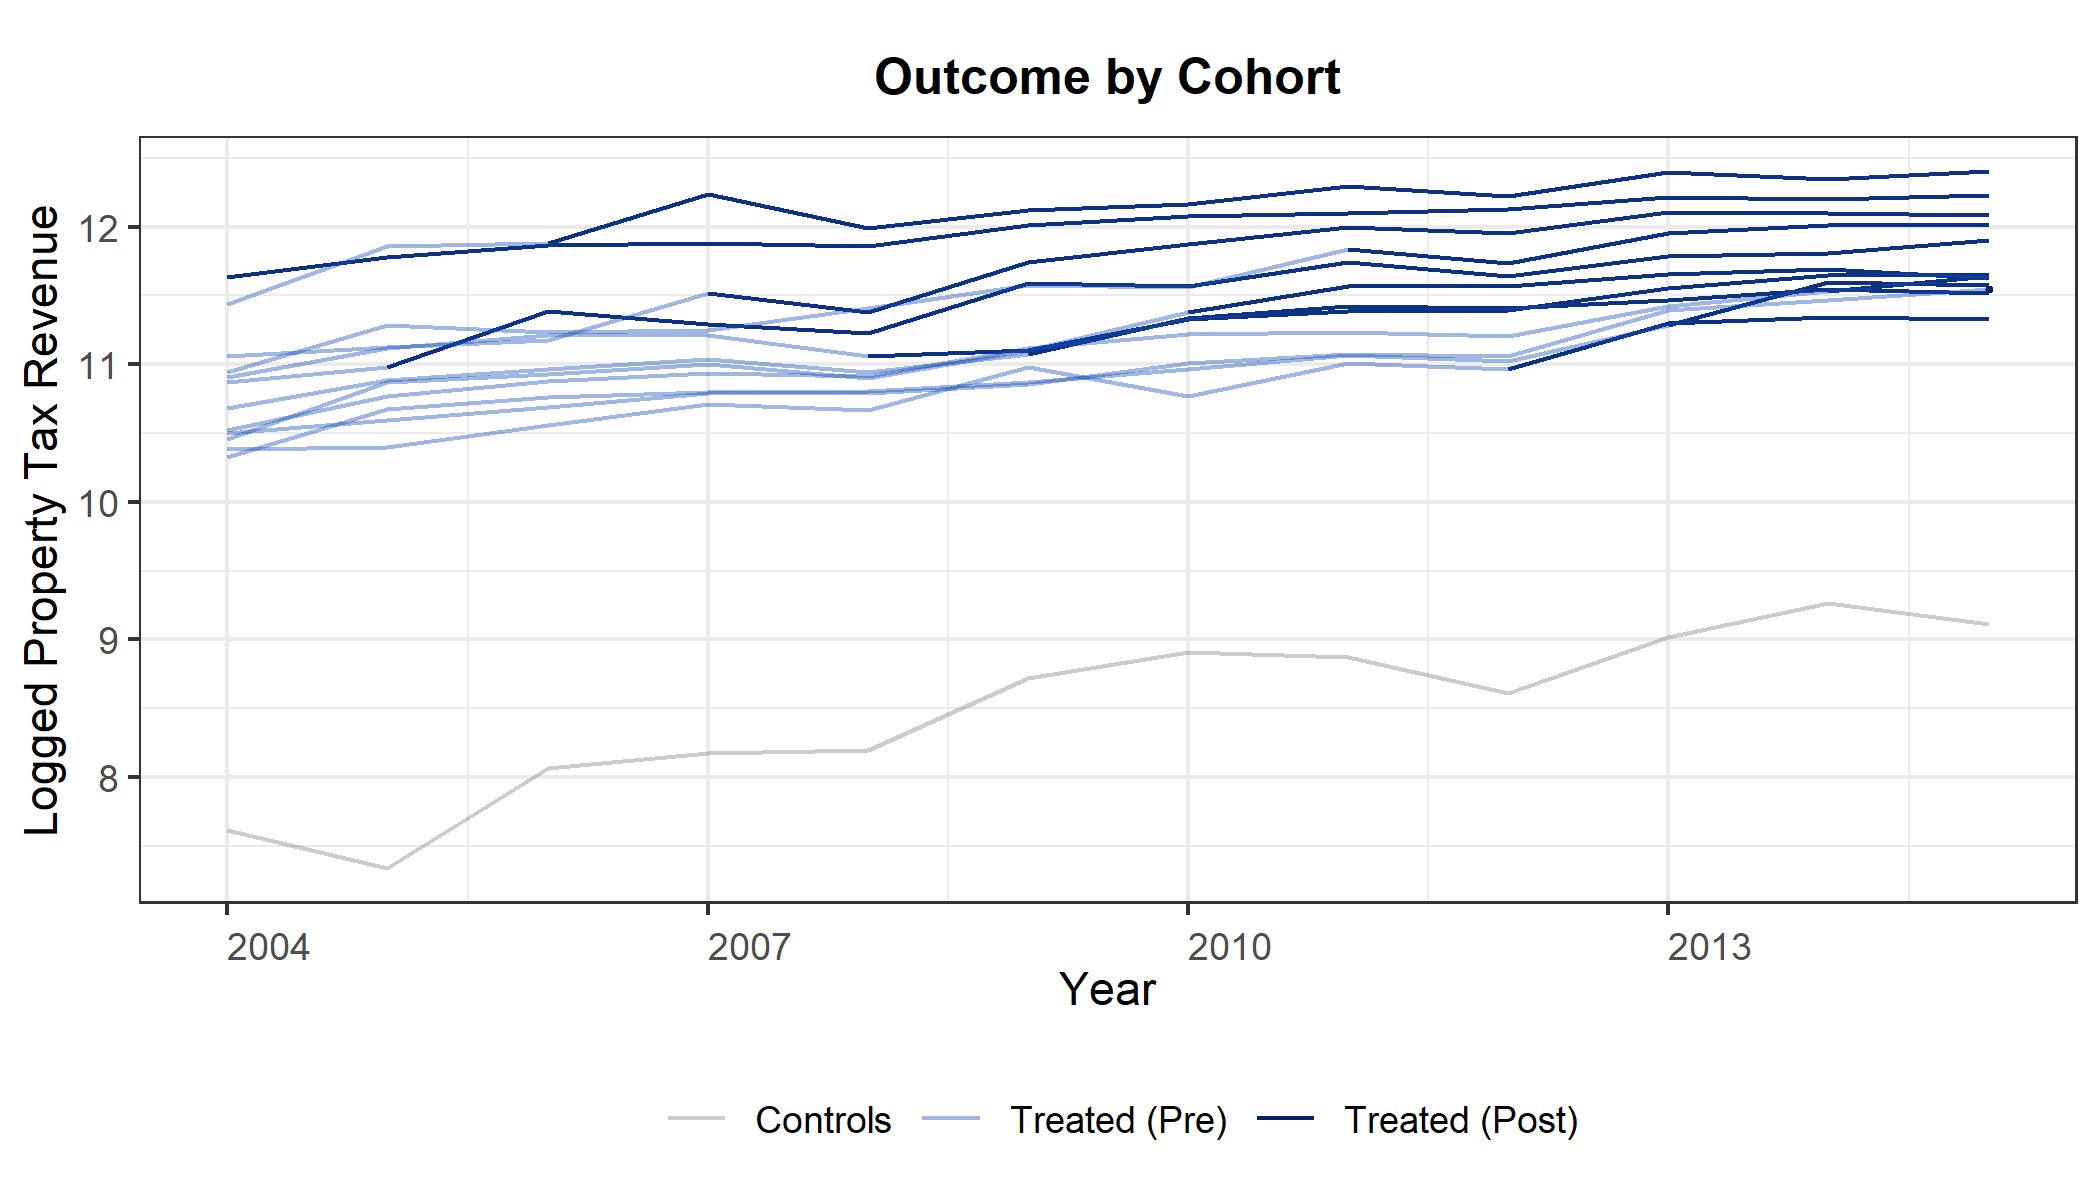
\includegraphics[width=\linewidth]{ex3_outcome_cohort.png}}
\end{column}
\begin{column}{0.62\textwidth}
\begin{itemize}\itemsep0.5em
\item<1-> A large \alert{always-treated} block sits on top of the staggered adopters; only a handful of municipalities are never treated
\item<2-> Those never-treated municipalities collect far less revenue than every treated cohort: a weak comparison group
\item<3-> Goodman-Bacon's decomposition of the TWFE estimate: comparisons among treated cohorts sit around $+0.25$, comparisons against the never-treated around $-0.4$; the answer depends on \alert{which comparisons carry weight}
\end{itemize}
\onslide<3->{\begin{center}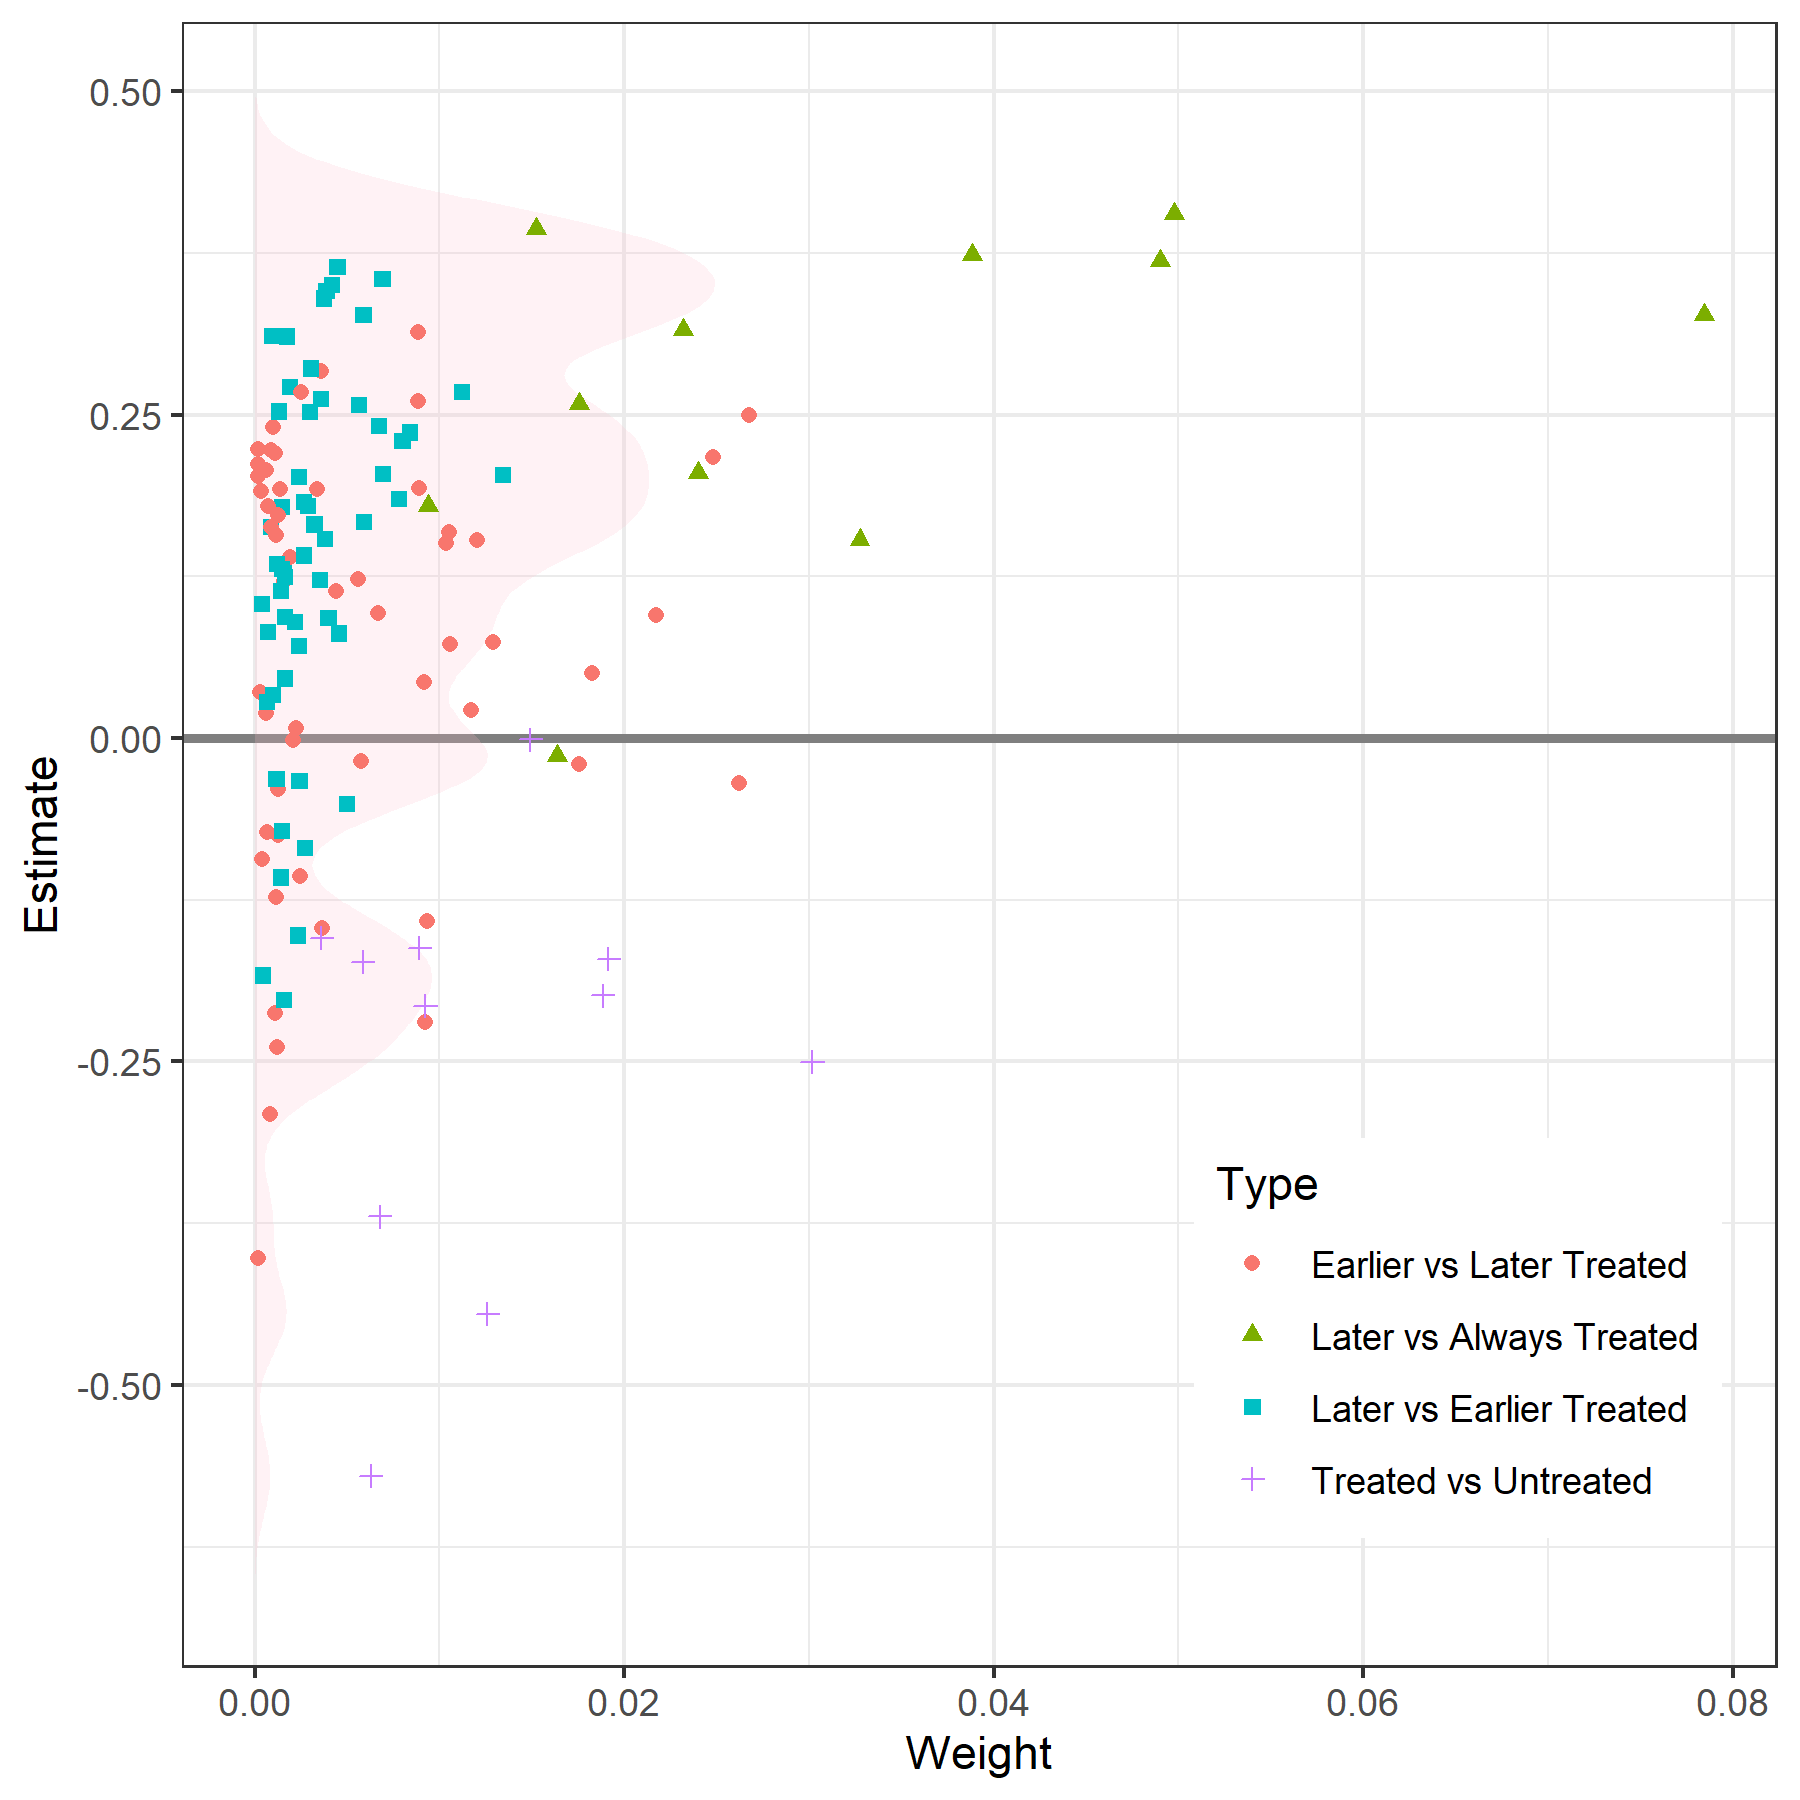
\includegraphics[height=0.36\textheight]{ex3_bacon_full.png}\end{center}}
\end{column}
\end{columns}
\end{frame}

\begin{frame}[t]
  \frametitle{Example 3: A Trimmed Subsample}
\begin{columns}[T,onlytextwidth]
\begin{column}{0.44\textwidth}\centering
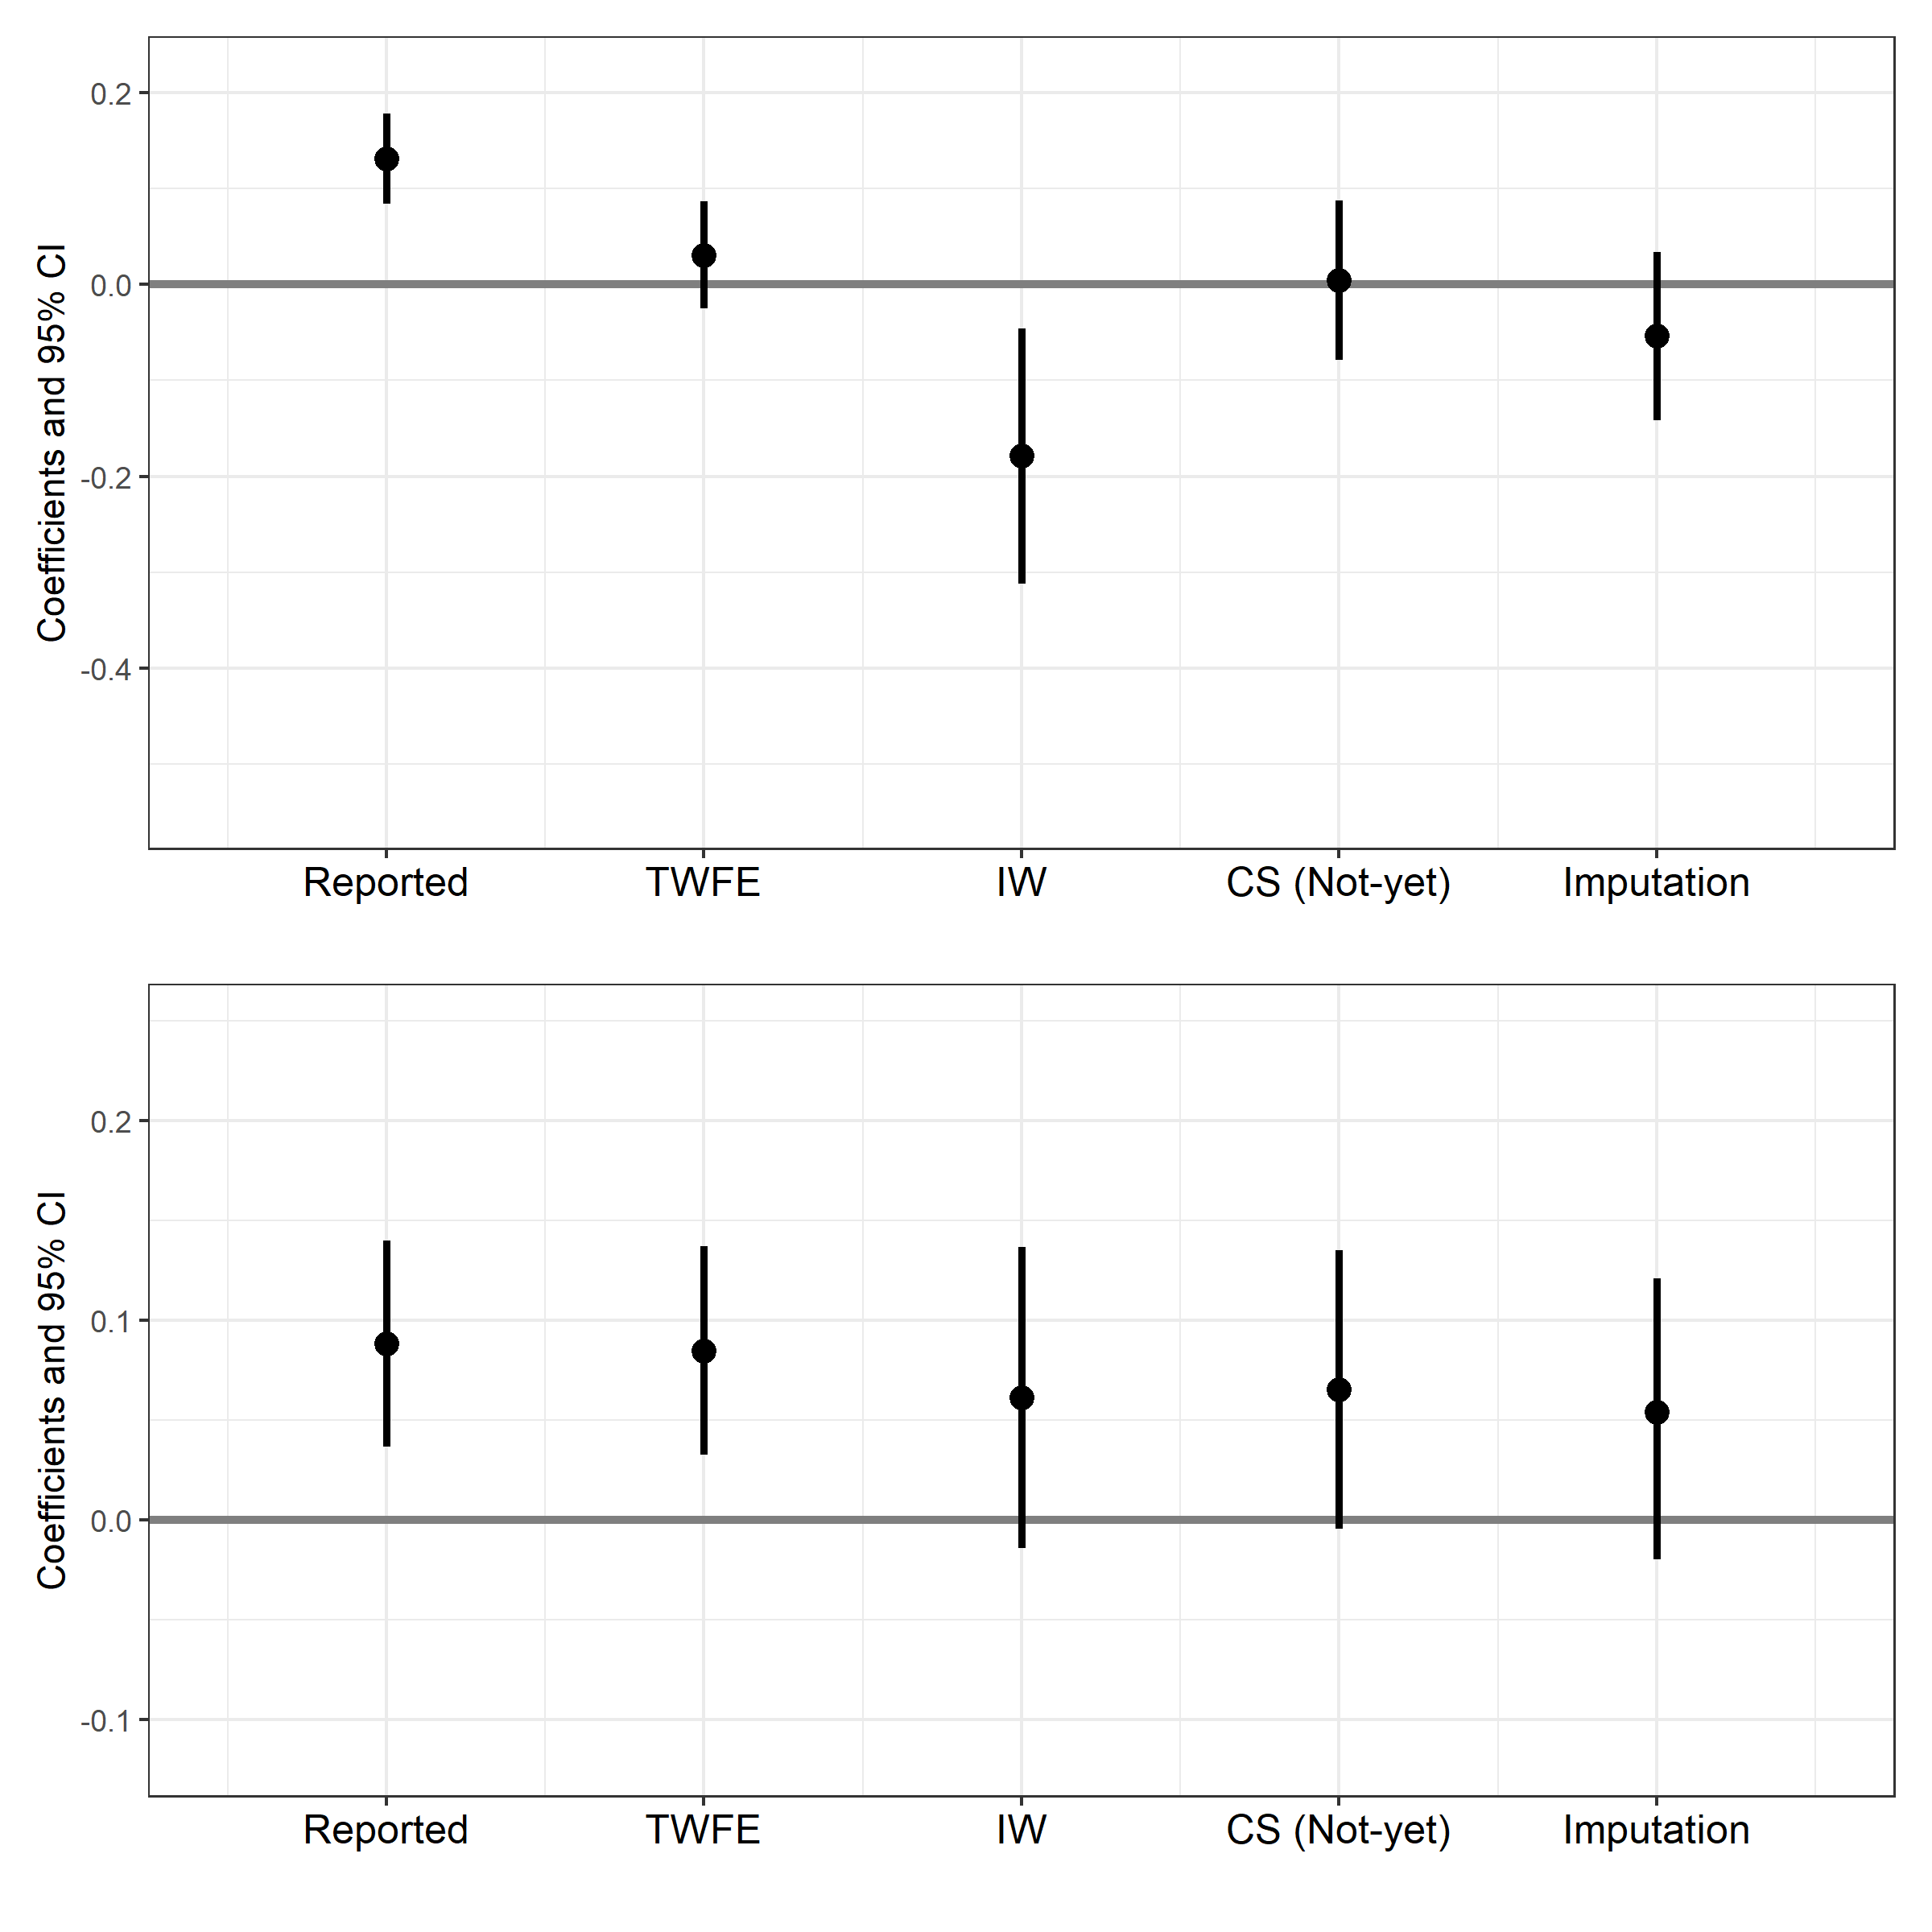
\includegraphics[width=\linewidth, height=0.7\textheight, keepaspectratio]{ex3_compare_full_sub.png}\par
{\scriptsize top: full sample; bottom: trimmed subsample}
\end{column}
\begin{column}{0.54\textwidth}
\begin{itemize}\itemsep0.5em
\item<1-> Drop the always-treated block and the far-away never-treated units, without looking at the outcome
\item<2-> On the subsample the estimators \alert{converge}, all between $0.05$ and $0.09$ with overlapping intervals; the comparisons now form one cloud
\item<3-> The disagreement was a symptom of a weak comparison set, not of heterogeneity; trimming to ``compare like with like'' is design work \parencite{imbens2015causal}
\end{itemize}
\onslide<2->{\begin{center}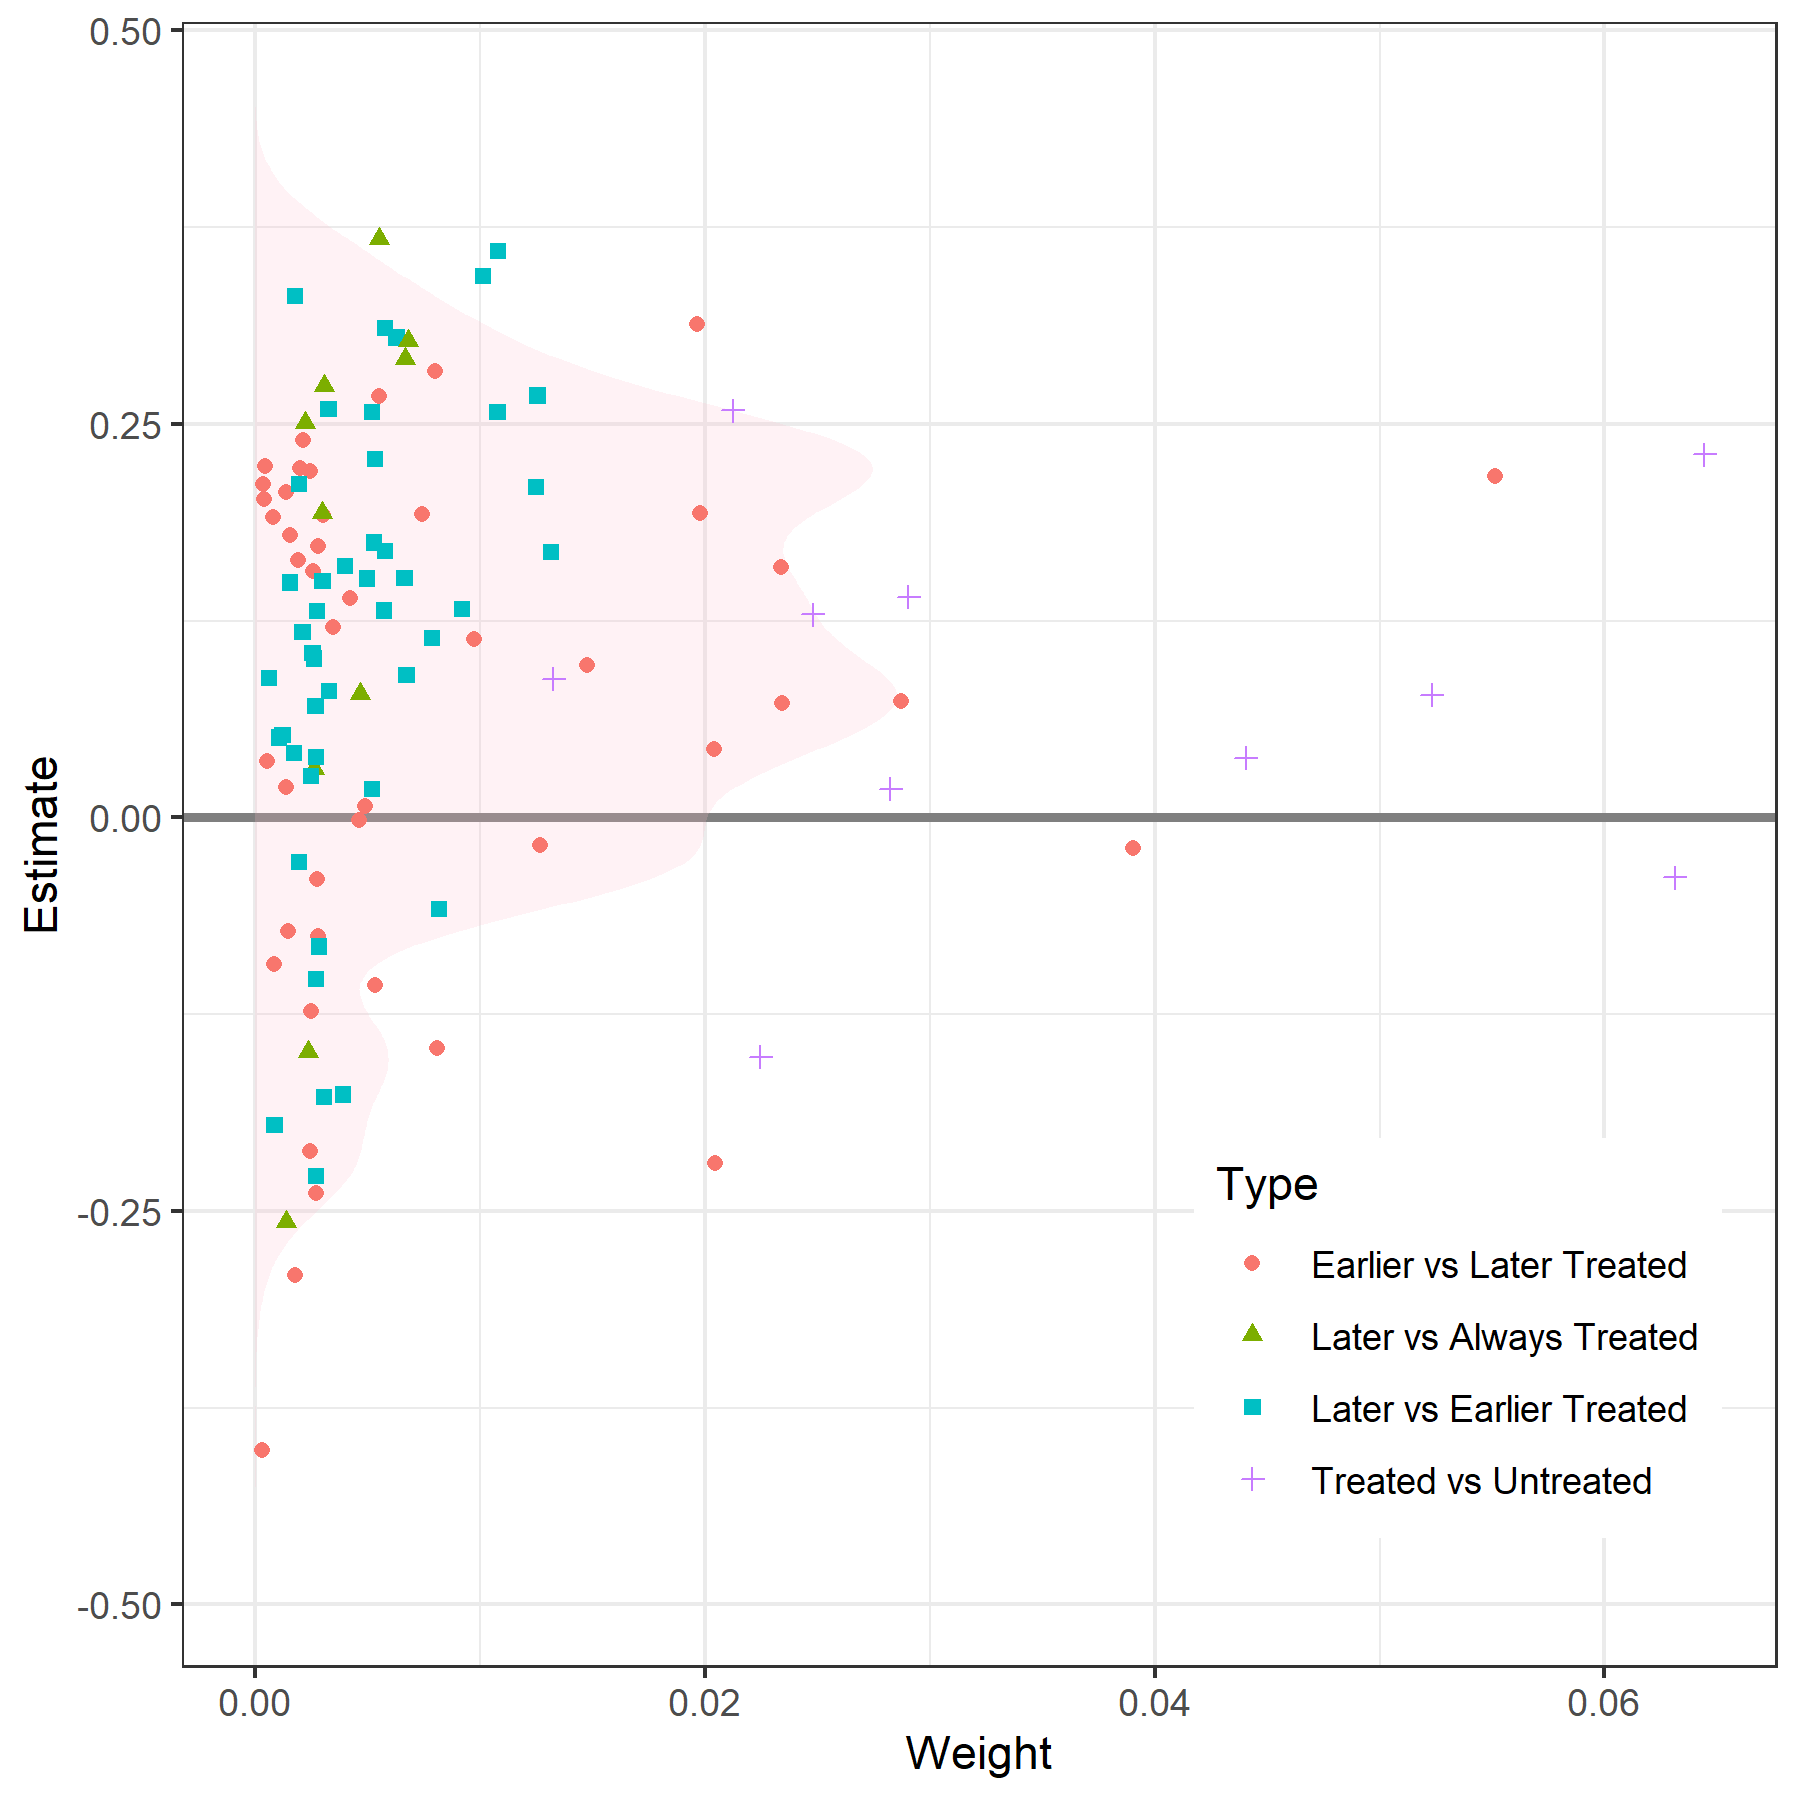
\includegraphics[height=0.35\textheight]{ex3_bacon_sub.png}\end{center}}
\end{column}
\end{columns}
\end{frame}

\begin{frame}
  \frametitle{Three Examples, Three Lessons}
\begin{itemize}[<+->]\itemsep1.1em
\item \textbf{Example 1, coethnic mobilization}: strong design; heterogeneity matters marginally; the estimators, TWFE included, broadly agree
\item \textbf{Example 2, land-use lawsuits}: clear signs of a parallel trends violation; heterogeneity is second-order; agreement among estimators does not mean robustness; plotting the raw data and the two tests spot the problem
\item \textbf{Example 3, cadastral maps}: when estimators disagree, suspect the comparison set before the estimators; design-phase trimming, done without the outcome, restores agreement
\end{itemize}
\end{frame}

\begin{frame}
  \frametitle{Carryover Effects Are Common}
\begin{columns}[T,onlytextwidth]
\begin{column}{0.5\textwidth}
\medskip
\begin{itemize}[<+->]\itemsep1em
\item With treatment reversal, effects that linger after exit violate the no-carryover assumption; we find this in roughly a third of the reanalyzed studies
\item When carryover is plausible, estimate effects relative to treatment \alert{entry} only, or model the exit explicitly
\end{itemize}
\end{column}
\begin{column}{0.48\textwidth}
\centering
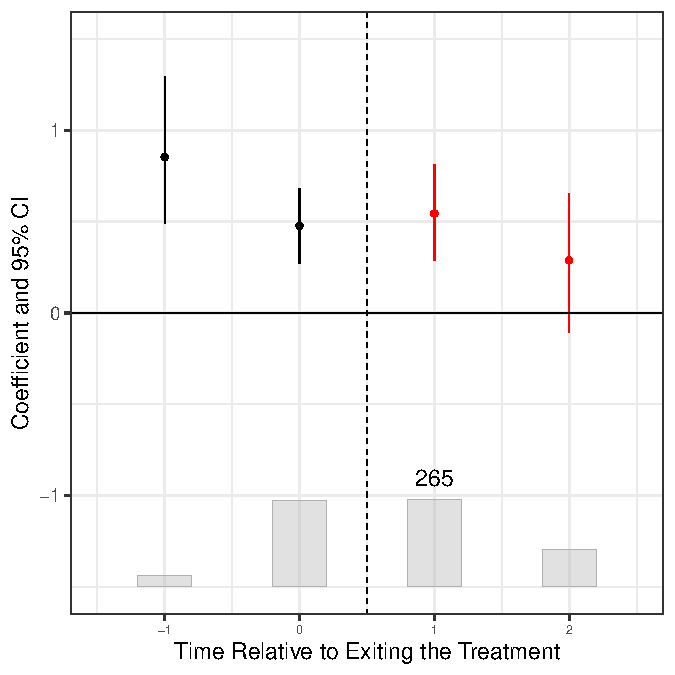
\includegraphics[width=\linewidth, height=0.66\textheight, keepaspectratio]{distelhorst_carryover.pdf}
\par{\scriptsize \textcite{distelhorst2018compliance}: rejects no carryover --- unlike Example 1 (\cite{grumbach2020race})}
\end{column}
\end{columns}
\end{frame}

\begin{frame}
  \frametitle{Sensitivity Analysis: Relaxing Parallel Trends}
\begin{itemize}\itemsep0.6em
\item \textcite{rambachan2023more}: allow post-treatment confounding up to $M$ times the largest change between neighboring placebo periods; $M = 0$ means parallel trends holds exactly
\end{itemize}
\medskip
\begin{columns}[T,onlytextwidth]
\begin{column}{0.49\textwidth}
\centering
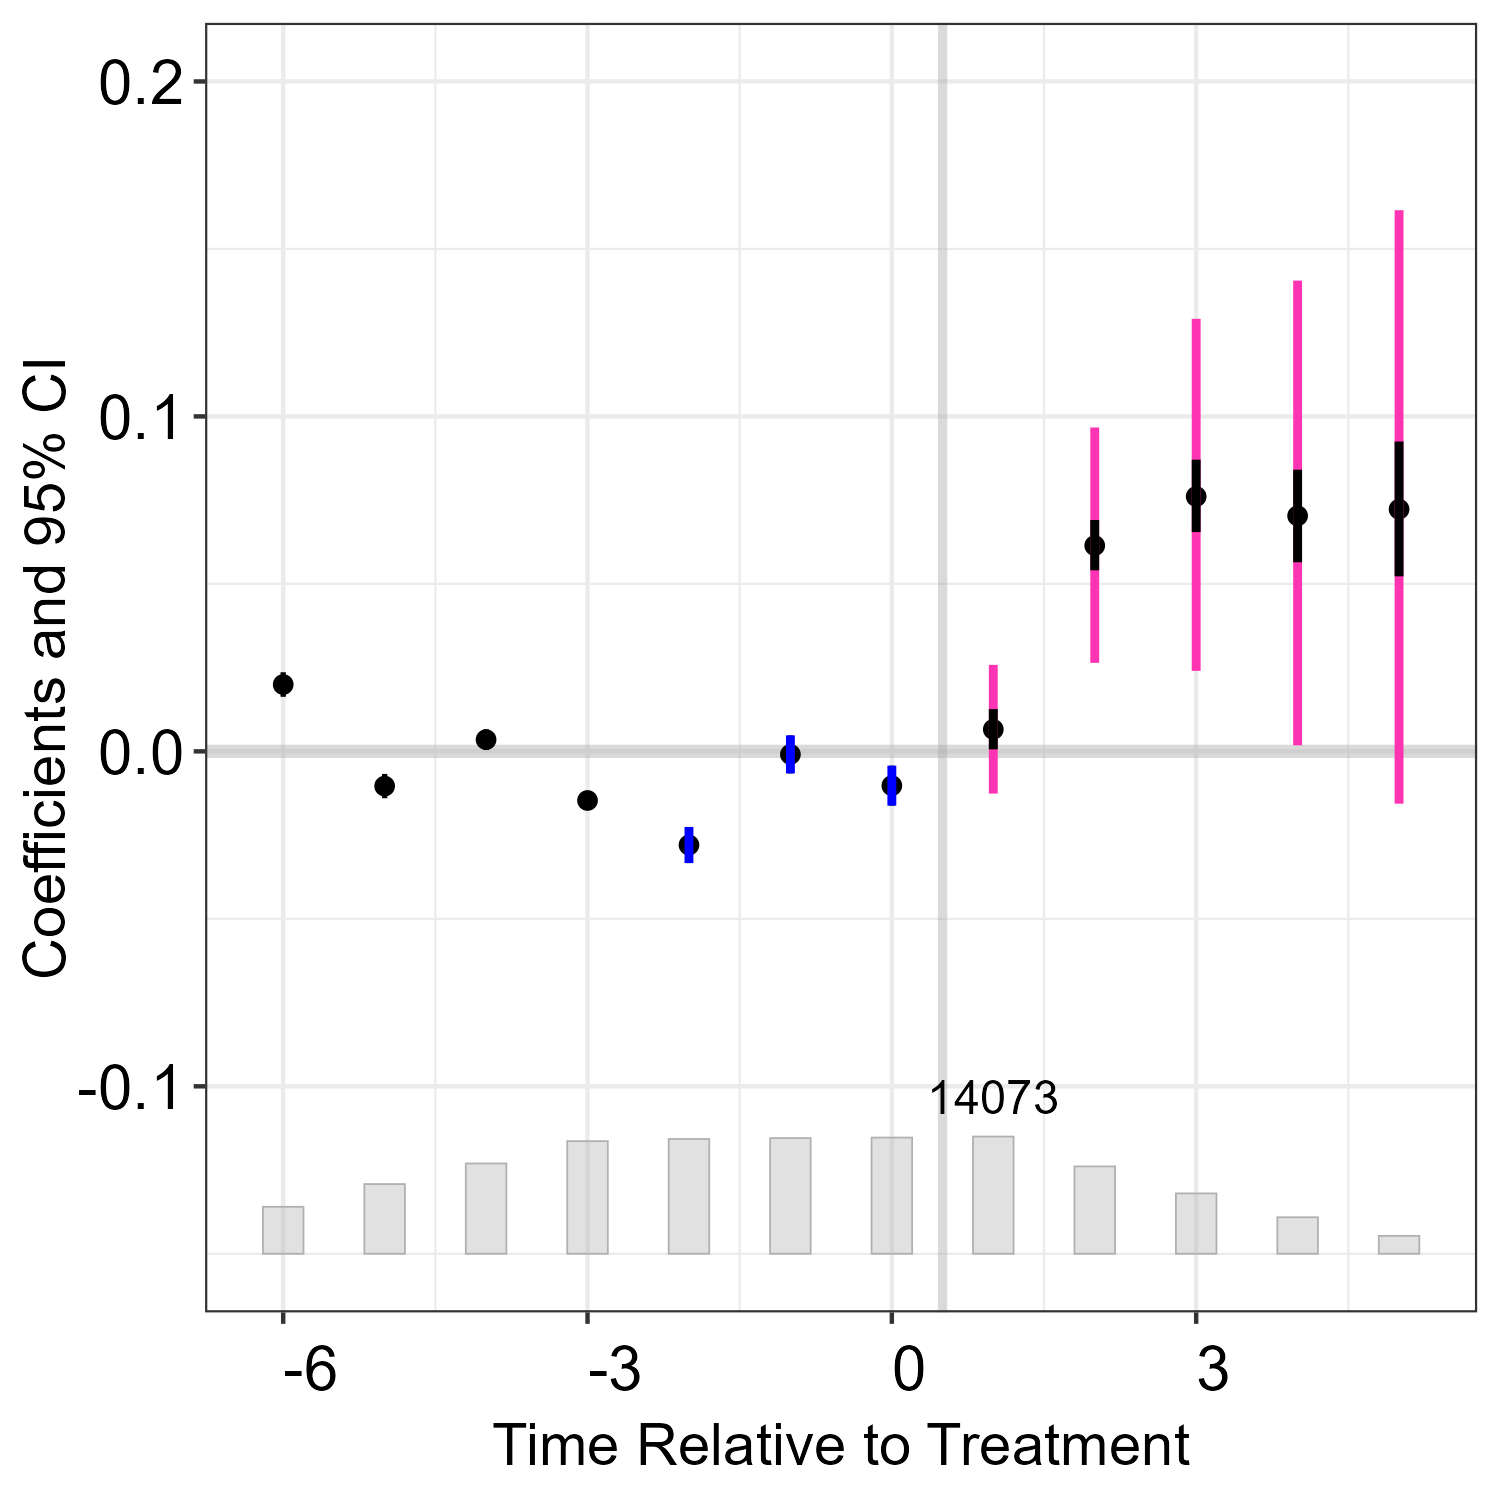
\includegraphics[width=0.92\linewidth, height=0.45\textheight, keepaspectratio]{hallyoder_honest.png}
\par{\scriptsize \textcite{hall2022homeownership}}
\end{column}
\begin{column}{0.49\textwidth}
\centering
\onslide<2->{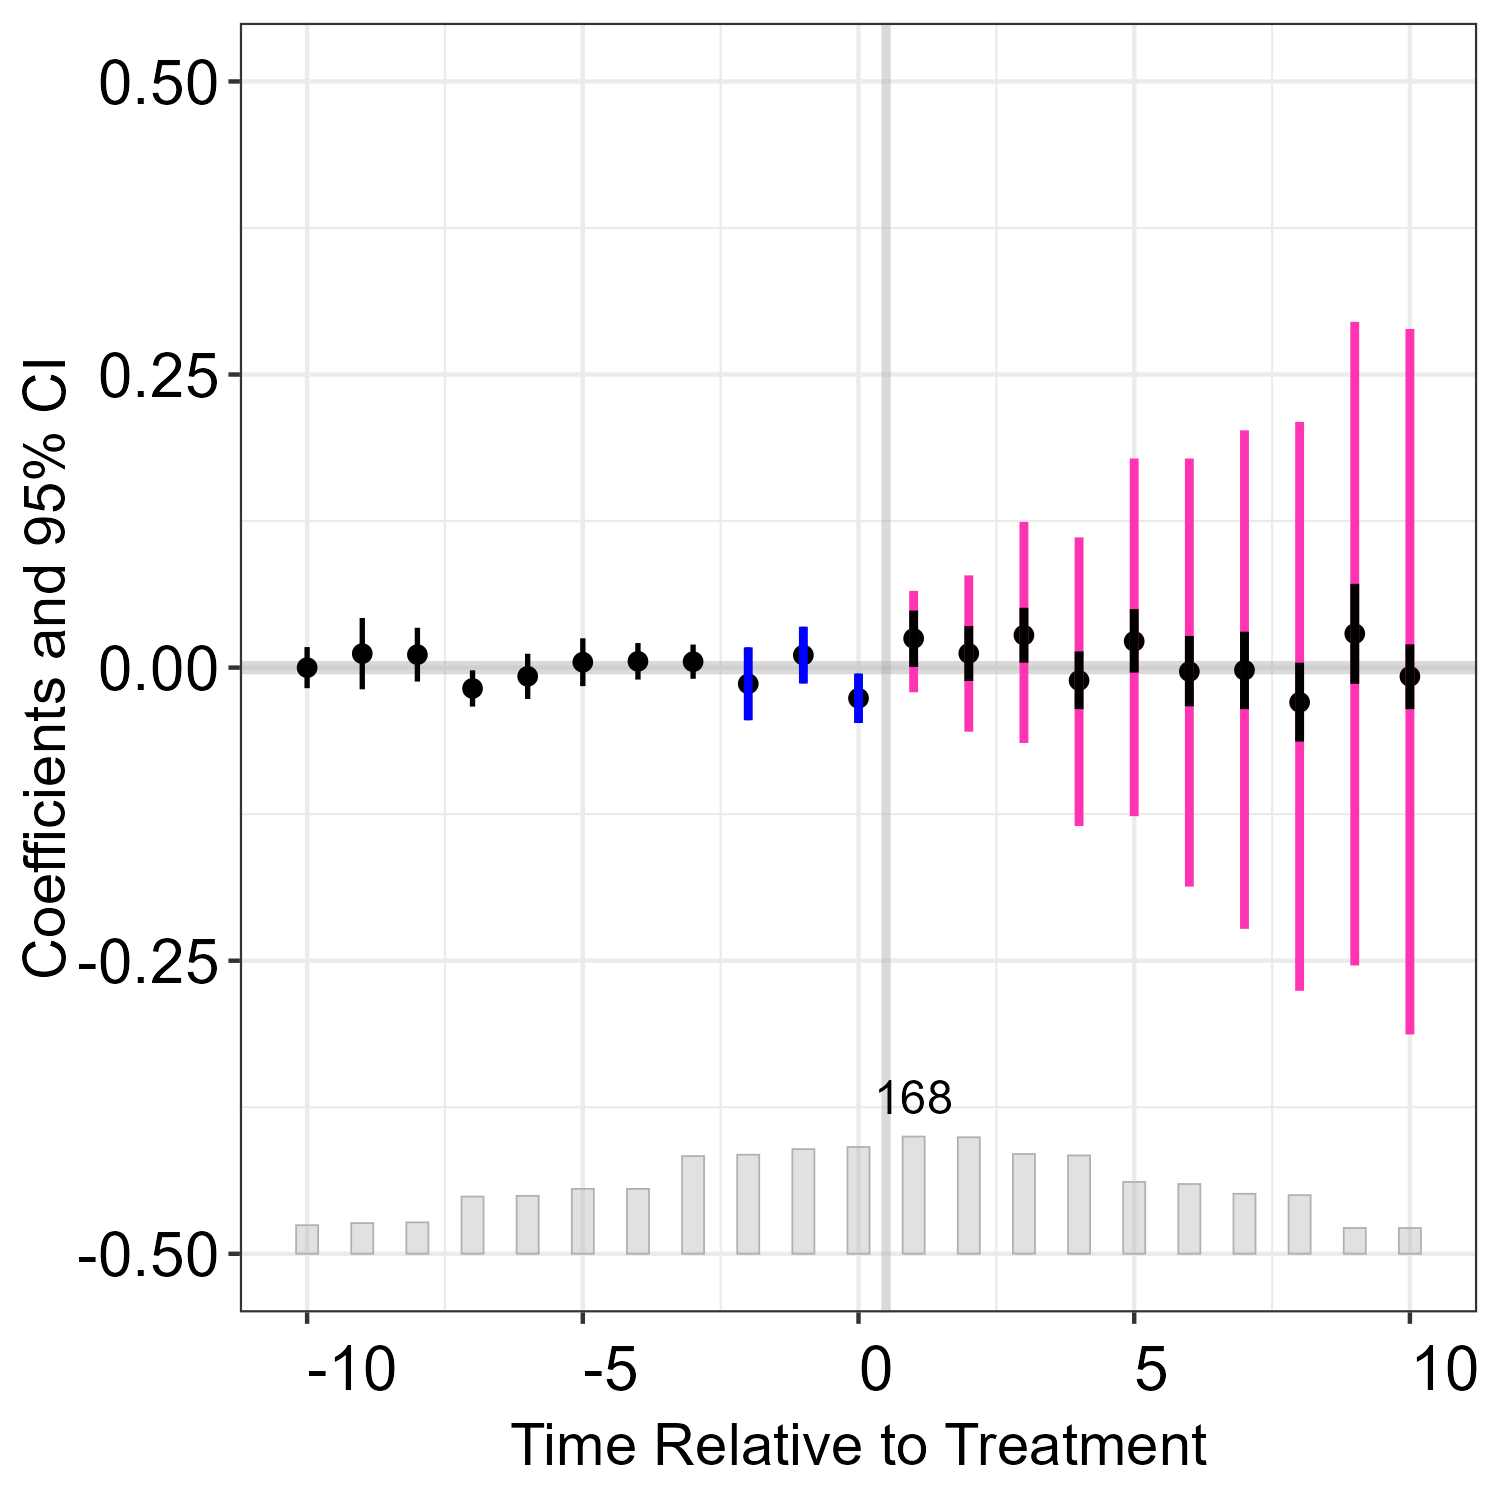
\includegraphics[width=0.92\linewidth, height=0.45\textheight, keepaspectratio]{caughey_honest.png}
\par{\scriptsize \textcite{caughey2017incremental}}}
\end{column}
\end{columns}
\bigskip
\begin{itemize}
\item<3-> The question shifts from ``does the effect exist'' to ``how much confounding would it take to erase it''
\end{itemize}
\end{frame}

\begin{frame}
  \frametitle{The Reanalysis Study (\citeall{chiu2026causal})}
\begin{itemize}[<+->]\itemsep0.9em
\item We replicated a main result from top political science journals, 2017--2023: 102 papers use linear panel models; 64 have a ``proper'' TWFE design; \alert{49 are replicable}
\item Each study re-estimated with the full menu: IW, CSDID, stacked, PanelMatch/DID$_M$, and imputation, plus the diagnostic suite and sensitivity analysis
\item Settings in the sample: 55\% general (with reversal), 27\% staggered, 12\% multi-period block, 6\% classic $2\times 2$: \alert{the staggered-only estimators do not even apply to most studies}
\end{itemize}
\end{frame}

\begin{frame}
  \frametitle{Finding 1: Estimates Rarely Flip, but Variability Exists}
\begin{center}
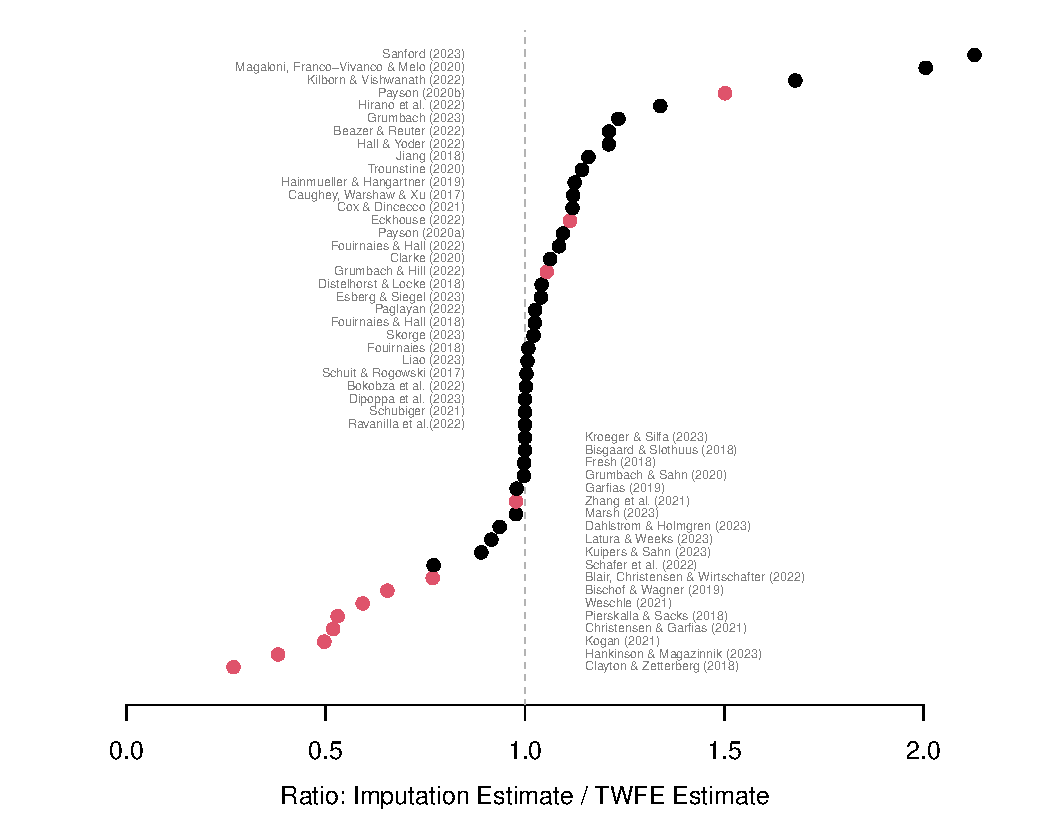
\includegraphics[height=0.68\textheight]{est_ratio2.pdf}
\end{center}
\begin{itemize}
\item<2-> The ratio of imputation to TWFE estimates centers on 1.0 (mean 1.02, median 1.00); large deviations concentrate in sparse-data cases
\end{itemize}
\end{frame}

\begin{frame}
  \frametitle{Finding 1 (continued): The Staggered Cases}
\begin{center}
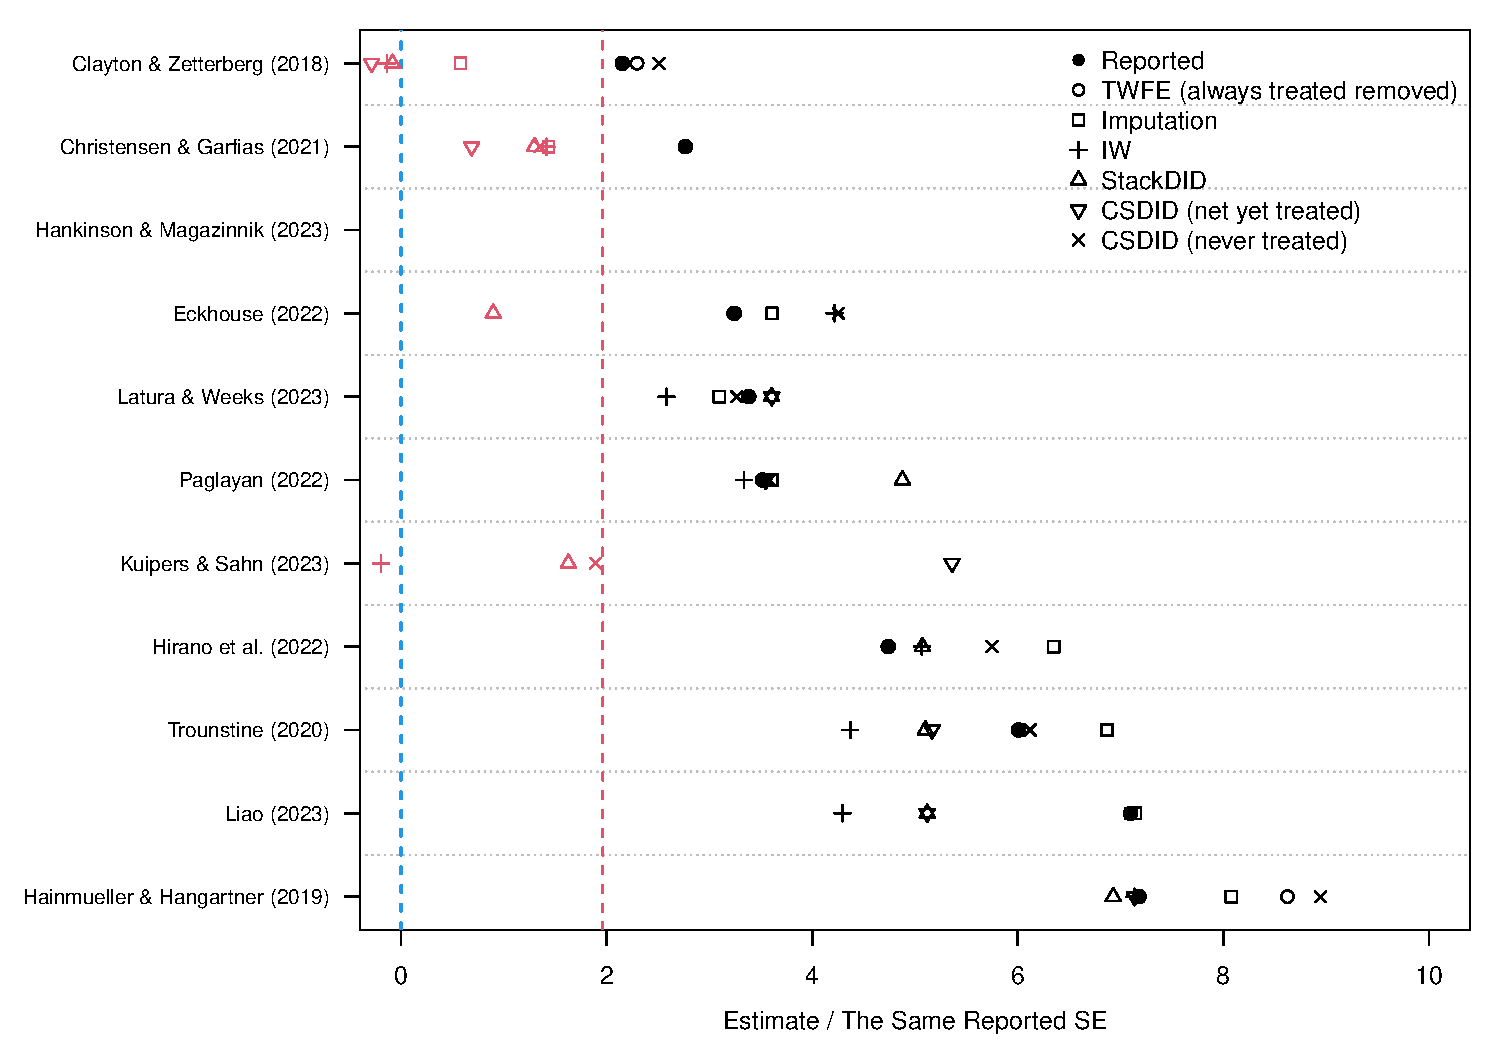
\includegraphics[height=0.7\textheight]{est_staggered_coef.pdf}
\end{center}
\begin{itemize}
\item<2-> Across the staggered studies, the five HTE-robust estimators and TWFE broadly agree on magnitudes
\end{itemize}
\end{frame}

\begin{frame}
  \frametitle{Finding 2: ``Robust'' DID Is Power Hungry}
\begin{columns}[T,onlytextwidth]
\begin{column}{0.32\textwidth}
\centering
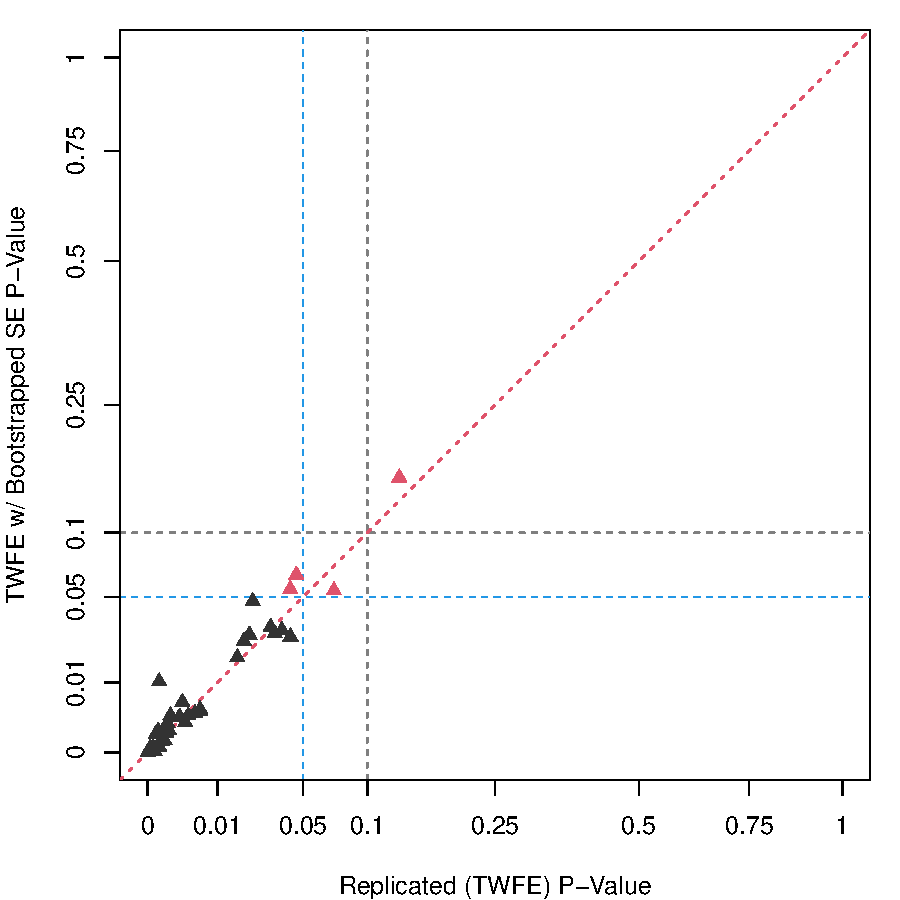
\includegraphics[width=\linewidth]{pvalues_twfe_boot.pdf}
\par{\scriptsize bootstrapped SEs (91\% survive)}
\end{column}
\begin{column}{0.32\textwidth}
\centering
\onslide<2->{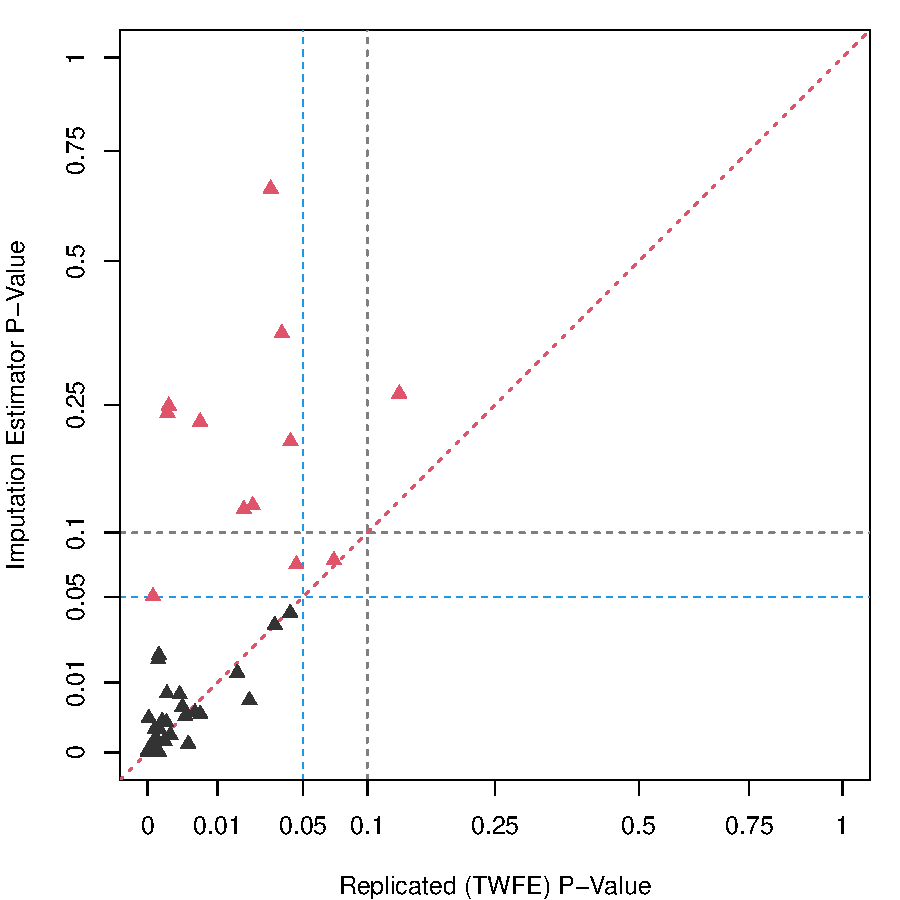
\includegraphics[width=\linewidth]{pvalues_fect.pdf}
\par{\scriptsize + relaxing constant effects (75\%)}}
\end{column}
\begin{column}{0.32\textwidth}
\centering
\onslide<3->{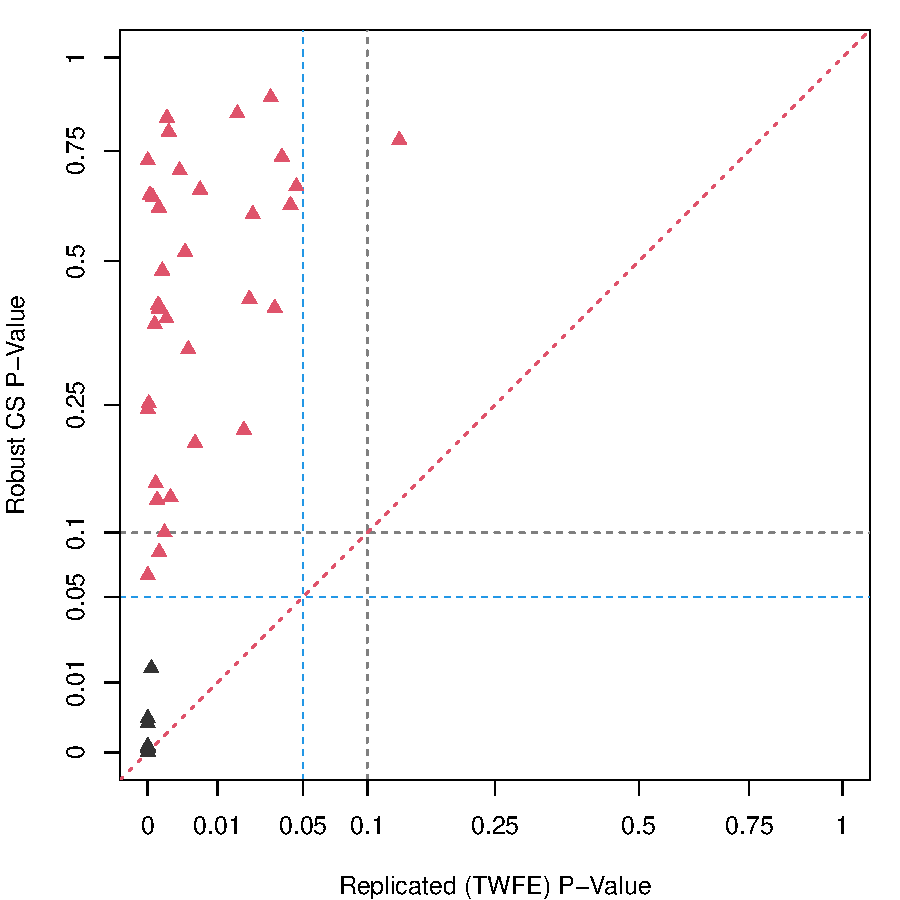
\includegraphics[width=\linewidth]{pvalues_robust.pdf}
\par{\scriptsize + relaxing parallel trends (23\%)}}
\end{column}
\end{columns}
\bigskip
\begin{itemize}
\item<4-> Each layer of robustness costs power; fewer than a third of the findings survive mild sensitivity analysis
\end{itemize}
\end{frame}

\begin{frame}
  \frametitle{Big Picture: Design and Power}
\begin{center}
\begin{tikzpicture}[scale=0.78]
\useasboundingbox (-6.5,-3.4) rectangle (6.5,3.3);
\only<4->{\fill[gray!15] (0,-1.5) ellipse (5.2 and 1.6);
  \node[font=\small, gray] at (-3.3,-2.35) {the fog of low power};}
\draw[-{Latex[length=2.5mm]}, thick, SlideInk] (-6,0) -- (6,0);
\draw[-{Latex[length=2.5mm]}, thick, SlideInk] (0,-3.2) -- (0,3.1);
\node[font=\small, anchor=east] at (-4.9,-0.35) {weak design};
\node[font=\small, anchor=west] at (4.9,-0.35) {strong design};
\node[font=\small, anchor=west] at (0.15,2.9) {high power};
\node[font=\small, anchor=west] at (0.15,-3.0) {low power};
\only<2->{\fill[SlideRed!25] (-3.4,1.7) ellipse (1.6 and 1.0); \node[font=\small] at (-3.4,1.7) {Example 2};}
\only<3->{\fill[SlideBlue!25] (3.4,1.7) ellipse (1.6 and 1.0); \node[font=\small] at (3.4,1.7) {Example 1};}
\only<4->{\node[font=\small] (e3) at (-1.3,-0.8) {Example 3};
  \node[font=\small] (e3s) at (3.4,-1.2) {Example 3$^*$};
  \draw[-{Latex[length=2mm]}, thick, SlideRed] (e3.east) to[bend left=18] (e3s.west);}
\end{tikzpicture}
\end{center}
\vspace{-0.4em}
\begin{itemize}
\item<5-> Estimator choice barely moves a study along either axis; \alert{design} and \alert{power} do. Trimming moved Example 3 to the right; moving up takes more data
\end{itemize}
\end{frame}

\begin{frame}
  \frametitle{The Paradox of Committing to TWFE}
\begin{itemize}[<+->]\itemsep1.2em
\item Clear signs of parallel trends violations in roughly a quarter of the studies; in over half, we \alert{cannot tell}, because there are too few pre-periods or too little power
\item With enough power, you can afford an HTE-robust estimator, so use one
\item Without enough power, you cannot \alert{validate} the assumptions TWFE needs anyway
\item Either way, blind TWFE is hard to defend; the binding constraints are \alert{design and power}, not the estimator
\end{itemize}
\end{frame}

\begin{frame}
  \frametitle{Recommendations}
\small
\begin{center}
\renewcommand{\arraystretch}{1.35}
\begin{tabular}{p{0.2\textwidth}p{0.36\textwidth}p{0.34\textwidth}}
 & \textbf{Do} & \textbf{Don't} \\ \hline
Design & Start from a research design; check for feedback from past outcomes & Start by running regressions on whatever data exist \\
Raw data & Plot treatment status and outcome trajectories first & Run regressions without looking at the data \\
Estimators & Use HTE-robust estimators; always plot dynamic effects & Choose models on belief; report coefficients only \\
Diagnostics & Run visual and statistical tests of the assumptions & Skip visualization and diagnostics \\
Clustering & Cluster at the level of treatment assignment or higher & Cluster below the assignment level \\
Small clusters & Cluster-bootstrap when clusters $\lesssim 50$ & Rely on asymptotic SEs \\ \hline
\end{tabular}
\end{center}
\end{frame}


\section{Conclusions}

\begin{frame}[t]
  \frametitle{Summary}
\begin{itemize}[<+->]\itemsep1.1em
\item The HTE-robust menu is organized by comparisons: DID extensions choose their $2\times 2$s explicitly; imputation methods model $Y(0)$ from untreated cells
\item In 49 reanalyses, estimator choice rarely flips results; parallel trends violations and \alert{low power} are the first-order problems
\item Run the diagnostic suite (pre-trend, placebo, carryover, equivalence) and report a sensitivity analysis, not just a point estimate
\end{itemize}
\end{frame}

\begin{frame}[t]
  \frametitle{Software}
\begin{itemize}\itemsep0.5em
\item \texttt{fect} (R \& Stata): imputation estimators with the full diagnostic suite
\item \texttt{panelView} (R \& Stata): treatment status and outcome visualization
\item \texttt{did}, \texttt{PanelMatch}, \texttt{DIDmultiplegt}: the DID extensions; \texttt{didimputation}: BJS imputation; \texttt{etwfe} (R) and \texttt{jwdid} (Stata): extended TWFE
\item Tutorials: \url{https://yiqingxu.org/tutorials/panel.html}
\end{itemize}
\end{frame}

\appendix

\setbeamertemplate{frametitle continuation}[from second][(cont.)]
\begin{frame}[t,allowframebreaks=1.1]
  \frametitle{References}
  \referencelist
\end{frame}


\end{document}
